\documentclass[11pt]{article}
\usepackage[T1]{fontenc}
\usepackage{lmodern}
\usepackage{amsmath,amssymb,amsthm,mathtools}
\usepackage[margin=1in]{geometry}
\usepackage{microtype}
\usepackage{booktabs}
\usepackage{tikz}
\usetikzlibrary{arrows.meta,positioning,fit,calc}
\usepackage[colorlinks=true,linkcolor=blue!50!black,citecolor=blue!50!black,urlcolor=blue!50!black]{hyperref}
\hypersetup{pdftitle={The Gaussian free field limit of the balanced six-vertex model with variance multiplier 1/arcsin(c/2)},pdfauthor={OpenAI}}
\numberwithin{equation}{section}
\newtheorem{theorem}{Theorem}[section]
\newtheorem{lemma}[theorem]{Lemma}
\newtheorem{proposition}[theorem]{Proposition}
\newtheorem{corollary}[theorem]{Corollary}
\theoremstyle{definition}
\newtheorem{definition}[theorem]{Definition}
\newtheorem{remark}[theorem]{Remark}
\newtheorem{example}[theorem]{Example}
\newcommand{\R}{\mathbb R}
\newcommand{\C}{\mathbb C}
\newcommand{\Z}{\mathbb Z}
\newcommand{\N}{\mathbb N}
\newcommand{\E}{\mathbb E}
\renewcommand{\P}{\mathbb P}
\newcommand{\bbone}{\mathbf1}
\newcommand{\one}{\mathbf1}
\newcommand{\dd}{\,\mathrm d}
\renewcommand{\Re}{\operatorname{Re}}
\renewcommand{\Im}{\operatorname{Im}}
\DeclareMathOperator{\supp}{supp}
\DeclareMathOperator{\tr}{tr}
\DeclareMathOperator{\Tr}{Tr}
\DeclareMathOperator{\Span}{span}
\DeclareMathOperator{\Dom}{Dom}
\DeclareMathOperator{\TV}{TV}
\DeclareMathOperator{\Cov}{Cov}
\DeclareMathOperator{\Var}{Var}
\DeclareMathOperator{\dist}{dist}
\DeclareMathOperator{\diam}{diam}
\DeclareMathOperator{\Lip}{Lip}
\DeclareMathOperator{\diag}{diag}
\DeclareMathOperator{\sech}{sech}
\DeclareMathOperator{\sgn}{sgn}
\newcommand{\ip}[2]{\langle #1,#2\rangle}
\newcommand{\norm}[1]{\left\lVert #1\right\rVert}
\newcommand{\abs}[1]{\left\lvert #1\right\rvert}
\allowdisplaybreaks[2]
\setlength{\emergencystretch}{2em}

\title{The Gaussian free field limit of the balanced six-vertex model\\ with variance multiplier \(1/\arcsin(c/2)\)}
\author{OpenAI}
\date{September 23, 2026}
\begin{document}
\maketitle
\begin{abstract}
We prove that the height function of the square-lattice six-vertex model
with weights \(a=b=1\) and \(0<c\le2\), in the plane state obtained from
balanced tori, converges to a multiple of the Gaussian free field.
For unit height jumps and Green kernel \(-(2\pi)^{-1}\log|x-y|\), the
squared multiplier is \(1/\arcsin(c/2)\).
\end{abstract}
\tableofcontents
\section{Introduction}\label{sec:introduction}

The six-vertex model assigns an arrow to each edge of the square lattice,
subject to the rule that two arrows enter and two arrows leave each vertex.
Its height function is a discrete random surface. We prove the Gaussian
free field limit of this surface throughout the critical range
\(a=b=1\), \(0<c\le2\), for the plane state specified below.

\subsection{The plane law and the height convention}

The two vertices having both horizontal arrows directed inward, or both
directed outward, have weight \(c\); the other four vertices have weight
one. A finite configuration has the product of its vertex weights.
On
\[
 T_{M,L}=(\Z/M\Z)\times(\Z/L\Z),\qquad M,L\ge4,\quad L\ \text{even},
\]
condition every vertical column of horizontal edges to contain \(L/2\)
left arrows and \(L/2\) right arrows. This is a conserved sector of the row
transfer matrix. We first take \(M\to\infty\), and then even \(L\to\infty\),
in the local weak topology of arrow configurations. We denote the resulting
plane law by \(\P_c\). Existence in the previously untreated range is part
of the theorem.

Give the face on the left of an arrow height one more than the face on its
right. The ice rule makes this a well-defined height \(h\), modulo an
additive constant, on the faces of the plane. For \(x=(x_1,x_2)\in\R^2\),
let \(h(x)\) be the height of the face with bottom-left corner
\((\lfloor x_1\rfloor,\lfloor x_2\rfloor)\), and set
\[
 h_\delta(x)=h(x/\delta),\qquad \delta>0.
\]
This convention also fixes the value on grid lines.

Let \(\Gamma\) be the real plane Gaussian free field modulo constants,
normalized by the Green kernel
\begin{equation}\label{eq:green}
 G(x,y)=-\frac1{2\pi}\log|x-y|.
\end{equation}
Thus its covariance on smooth compactly supported tests of total integral
zero is the integral of \(G\) against their product.
For compactly supported finite signed measures \(\mu,\nu\) of total mass
zero, write
\[
 \mathcal E(\mu,\nu)=\iint G(x,y)\,\mu(\dd x)\nu(\dd y).
\]
We say that \(\mu\) has finite energy if
\[
 \iint \log_+\frac1{|x-y|}\,|\mu|(\dd x)|\mu|(\dd y)<\infty,
 \qquad \log_+t=\max(\log t,0).
\]
For compactly supported finite signed measures, this is equivalent to
requiring \(\mathcal E(\mu,\mu)\) to be an ordinary finite
signed-measure integral. In particular, the definition does not allow
cancellation between infinite positive and negative energies.

\begin{theorem}\label{thm:main}
For every fixed \(c\in(0,2]\), the prescribed iterated balanced-torus limit
\(\P_c\) exists. Define
\begin{equation}\label{eq:multiplier}
 \Delta=1-\frac{c^2}{2},\qquad
 \sigma(c)^2=\frac2{\arccos\Delta}=\frac1{\arcsin(c/2)}.
\end{equation}
As \(\delta\downarrow0\) through arbitrary positive real values,
the fields \(h_\delta\) converge to
\(\sigma(c)\Gamma\) in each of the following senses.
\begin{enumerate}
\item For every finite family \(\mu_1,\ldots,\mu_m\) of compactly supported
finite signed measures of total mass zero and finite energy,
\[
 \bigl(\langle h_\delta,\mu_j\rangle\bigr)_{j=1}^m
 \ \Longrightarrow\
 \mathcal N\!\left(0,
       \bigl(\sigma(c)^2\mathcal E(\mu_i,\mu_j)\bigr)_{i,j=1}^m\right).
\]
\item For every bounded open \(U\subset\R^2\) and \(-1<\alpha<0\),
there is convergence in law, with tightness, in the ordinary restriction
spaces
\[
 \mathcal C^\alpha_{\mathrm{res}}(U):=B^\alpha_{\infty,\infty}(U),
 \qquad B^\alpha_{p,q}(U),\qquad W^{\alpha,p}(U),
 \quad 1\le p<\infty,\quad 1\le q\le\infty,
\]
modulo constants. Convergence also holds in the outward completion
\eqref{eq:source-holder} defined below. No regularity of
\(\partial U\) is required. One may fix a smooth compactly supported
\(\rho\) of integral one and replace each field \(X\) by
\(X-\langle X,\rho\rangle\), using the same pinning for the limit.
\item For every \(k\ge1\) and every tuple
\((u_i,u_i')_{i=1}^k\) with
\(\{u_i,u_i'\}\cap\{u_j,u_j'\}=\varnothing\) for \(i\ne j\),
\begin{equation}\label{eq:increment-main}
 \E_c\prod_{i=1}^k
    \bigl(h_\delta(u_i')-h_\delta(u_i)\bigr)
 \longrightarrow
 \sigma(c)^k\sum_{\pi}\prod_{\{i,j\}\in\pi}C_{ij},
\end{equation}
where the sum is over pairings of \(\{1,\ldots,k\}\), is zero for odd \(k\),
and
\[
 C_{ij}=G(u_i',u_j')-G(u_i',u_j)-G(u_i,u_j')+G(u_i,u_j).
\]
The convergence is uniform on compact sets of such tuples.
\end{enumerate}
\end{theorem}

The theorem concerns this particular zero-slope plane state. It makes no
uniqueness assertion among all Gibbs states or all slopes, and no estimate
uniform as \(c\downarrow0\).

\paragraph{Regularity conventions.}
The restriction spaces in part~2 are restrictions of the corresponding
whole-plane distribution spaces, with their quotient norms. For
\(W^{\alpha,p}\) we include both the Bessel-potential and the
negative Slobodeckij realizations. The Hölder
laws are supported on the separable closure of smooth functions. This
choice makes the statement meaningful on every bounded open set without
an extension theorem for its boundary. We also prove convergence in the
intrinsic dual spaces \((W^{s,p'}(U))^*\), for \(0<s<1\) and
\(1\le p<\infty\), where the fractional seminorm uses
only pairs of points of \(U\); see Proposition~\ref{prop:intrinsic-dual}.

The outward convention is the literal seminorm of
\cite[Definition~2.6(iii)]{DKLM2026}. Let \(\mathcal T_1(Q)\), with
\(Q=(-1,1)^2\), consist of compactly supported signed densities in \(Q\),
of integral zero, whose zero extensions are \(1\)-Lipschitz. Set
\begin{equation}\label{eq:source-holder}
 \|f\|_{\mathrm{out},\alpha,U}
 =\sup_{\substack{0<\varepsilon\le1,\ \varphi\in\mathcal T_1(Q)\\
                   \supp\varphi\subset U/\varepsilon}}
   \varepsilon^{-\alpha}
   \left|\int f(x/\varepsilon)\varphi(x)\,\dd x\right|.
\end{equation}
Here \(U\) indexes the allowed tests of the global plane field;
the sampled points \(x/\varepsilon\) need not lie in \(U\).
The space is the completion of \(C_c^\infty(\R^2)\) modulo the
kernel of this seminorm.
The absolute value leaves the source convention unchanged because
the test family is symmetric. Its convergence requires a separate
argument from convergence in restriction spaces.

\subsection{Prior work and the new ingredients}

At \(c=1\), Lieb computed the exact square-ice entropy~\cite{Lieb1967}.
The Gaussian description of critical six-vertex heights and the prediction
of its coupling belong to the Coulomb-gas approach. In the F-model regime
\(1<c<2\), Di Francesco, Saleur and Zuber~\cite[Section~2.3]{DFSZ1987}
give a Gaussian-action prediction which, after converting their height
steps of \(\pi/2\) to unit steps, agrees with \eqref{eq:multiplier}.
This physics prediction is distinct from convergence in the measure
classes and distribution topologies of Theorem~\ref{thm:main}.

At the free-fermion point \(c=\sqrt2\), a dimer representation makes
the correlations determinantal. Kenyon's conformal-invariance and GFF
theorems for domino tilings~\cite{Kenyon2000,Kenyon2001} are foundational
scaling-limit results in this setting. The periodic dimer Gibbs measures,
surface tension and logarithmic fluctuations studied by Kenyon, Okounkov
and Sheffield~\cite{KOS2006} describe the corresponding plane-state
picture. Near the free-fermion point, Falco~\cite{Falco2013} derived
arrow-correlation asymptotics and logarithmic height variance for the
isotropic six-vertex model through an interacting-fermion representation.
Giuliani, Mastropietro and Toninelli proved GFF convergence for a symmetric
weakly interacting dimer model~\cite{GMT2017} and the relation between its
height amplitude and correlation exponent~\cite{GMTHaldane2017}.
Their later treatment of tilted profiles~\cite[Section~2.3 and Theorem~2]{GMT2020}
includes the six-vertex interaction and establishes height-covariance and
amplitude identities near the free-fermion point; its Remark~5 leaves the
higher-cumulant extension needed for a full GFF theorem undeveloped.

Duminil-Copin, Kozlowski, Krachun, Manolescu and
Tikhonovskaia~\cite{DCKKMT2022} proved existence and condensation of Bethe
roots and obtained the free energy and its expansion near half filling.
Duminil-Copin, Karrila, Manolescu and Oulamara~\cite{DCKMO2024} proved
logarithmic delocalization for \(1\le c\le2\), using crossing estimates
and free-energy information. Lis~\cite{Lis2021} developed the
Baxter--Kelland--Wu representation for multi-point spin correlations and
proved infinite-volume and delocalization results on subintervals of this
range. Glazman and Lammers~\cite{GlazmanLammers2025} subsequently obtained
delocalization, including logarithmic bounds in the isotropic case, by
percolation methods. These results establish the scale of fluctuations;
identifying their joint law requires additional information. The
variational framework of Sheffield~\cite{Sheffield2005} and the strict
convexity theorem of Lammers and Tassy~\cite{LammersTassy2024} provide the
equilibrium tools used below when \(c\ge1\).

Duminil-Copin, Kozlowski, Lammers and Manolescu~\cite{DKLM2026} give a
nonperturbative GFF theorem on \(\sqrt3\le c\le2\), with the exact
multiplier \eqref{eq:multiplier}. Their proof combines transfer-matrix
spectral representations and reflection positivity with rotational
invariance and regularity estimates. The rotational-invariance input is
listed as in preparation in the cited version. We retain the use of
transfer spectra and reflection, but for \(0<c<2\) construct the two
Gaussian currents from finite row identities and uniform thermodynamic
estimates. At \(c=2\), Appendix~\ref{sec:endpoint-rotation} supplies the
needed rotational-invariance statement from the independent fair
orientations of FK loops, the plane loop correspondence of~\cite{Lis2021},
and the homotopy coupling underlying the FK rotation theorem
of~\cite{DCKKMO2026Rotation}. The remaining endpoint
argument uses~\cite{DKLM2026}. Its conditional amplitude theorem is also
used on \(1\le c<2\), after convergence has been established. Thus the
full-range statement concerns precisely the balanced plane law defined
above, with its normalization fixed in physical height units.

The finite algebra is the algebraic Bethe ansatz. The norm determinant
goes back to Gaudin, McCoy and Wu~\cite{GaudinMcCoyWu1981} and
Korepin~\cite{Korepin1982}; the scalar-product formula is due to
Slavnov~\cite{Slavnov1989}. We use its trigonometric and diagonally
twisted forms as developed by Kitanine, Maillet and
Terras~\cite{KMT1999} and Kitanine, Maillet, Slavnov and
Terras~\cite{KMST2005}. These exact finite identities are the algebraic
input. Uniform control as the row length grows is a separate analytical
problem, addressed in Section~\ref{sec:thermodynamic}.

Three estimates connect this finite algebra to the limiting field.
Root-tail control and an edge maximum principle give uniform inverses
for Gaudin matrices and for mixed discrete--continuous quadrature
operators. Finite-dimensional residue conditions then control simultaneous
escapes of several rapidities in the determinant formulas. Next, bounds
on the zeros of angular spectral functions outside two separated scale
windows justify the limiting holomorphic and antiholomorphic currents.
Finally, when \(c<1\), a homogeneous stiffness lower bound and a
staggered vacuum-overlap upper bound identify the same covariance
coefficient. This last step supplies the normalization where the
conditional probabilistic input is unavailable. Moment estimates and
desmoothing pass from the currents to the test classes and separated
increments in Theorem~\ref{thm:main}.

\subsection{Proof overview}\label{sec:overview}

For \(0<c<2\), introduce
\[
 \lambda=\arccos(-\Delta)\in(0,\pi),
 \qquad \eta=\lambda/\pi.
\]
Section~\ref{sec:finite} defines commuting row operators and their diagonal
marks, which record height increments. Section~\ref{sec:thermodynamic}
constructs their limiting matrix elements, proves uniform tail bounds,
and shows that words with widely separated angular parameters decorrelate.
A positive full-line resolvent gives uniform density comparisons for
every fixed positive \(\lambda\), including the small-\(\lambda\) range.

These matrix elements define a Hilbert space with commuting angular rows
in Section~\ref{sec:angular}. Their joint spectral values are inner functions
of a complex row parameter. The finite folded-row continuation argument
in Lemma~\ref{lem:scalar-continuation} gives a common analytic neighborhood;
canonical inner-function factorization describes the possible zeros and
boundary singularities~\cite{AiDongJiang2019}. A mark acts as a current.
The finite mass
\(\kappa\) of the spectrum transverse to common angular dilation is the
coefficient of the logarithmic height covariance. Section~\ref{sec:normalization}
computes \(\kappa\) directly when \(c<1\); for \(c\ge1\) the cited conditional
normalization theorem applies once convergence has been established.

Section~\ref{sec:chiral} separates the angular spectrum into two scales and
proves the Wick rules for the limiting currents. Section~\ref{sec:probability}
passes from these currents to smooth tests, separated point increments
and finite-energy measures, then proves convergence in negative
regularity spaces. Its wavelet
argument uses compactly supported wavelets~\cite{Daubechies1988} and
the classical Besov coefficient characterization in the form of
\cite[Proposition~2.3]{HairerLabbe2017}; restriction from the plane avoids
any regularity assumption on the boundary of \(U\).
The final proof combines the interval \(0<c<2\) with the endpoint
argument of Appendix~\ref{sec:endpoint-rotation}. Each thermodynamic
passage specifies which size tends to infinity first.

\section{Finite rows and their scalar products}\label{sec:finite}

The first step is finite-dimensional.  We express every fixed word of
marked rows as a finite sum of determinants on the Bethe roots, with all
normalizing factors specified.  The construction of those roots and the
estimates needed to pass to infinite volume are deferred to
Section~\ref{sec:thermodynamic}.  In particular, no completeness assertion
for Bethe eigenvectors is used in this section.

\subsection{The physical row and the standard monodromy}

The algebra below holds for $0<\lambda<\pi$, corresponding to the
open parameter interval $0<c<2$. The endpoint $c=2$ is treated
separately in Appendix~\ref{sec:endpoint-rotation}. Set
\begin{equation}\label{eq:spectral-coordinates}
 \lambda=\arccos(-\Delta),\qquad \eta=\lambda/\pi,\qquad
 v=\pi/2,\qquad x=i\eta z,\qquad w=e^{iz}.
\end{equation}
The physical time angle is $z=0$, increasing time points east, and the
space angle is $v$, increasing space points north.  Thus a common
imaginary translation of the $z$ arguments is a common real translation
of their $x$ arguments.  At a path step, the spin is $+1$ when the arrow
points along its left normal; the height increment is minus that spin.
These conventions fix the sign of every marked row.

Let $L$ be even and let $b_0,\ldots,b_{L-1}$ be real numbers.  On
$\mathcal H_L=(\C^2)^{\otimes L}$ use the orthonormal spin basis, and put
\[
 Z=\begin{pmatrix}1&0\\0&-1\end{pmatrix},\qquad
 X=\begin{pmatrix}0&1\\1&0\end{pmatrix}.
\]
An auxiliary copy of $\C^2$ is denoted by the subscript $a$.  Products
over the sites below have increasing site index from left to right.  Define
\begin{align}
 R(u)&=
 \begin{pmatrix}
 \sin(\lambda-u)/\sin\lambda&0&0&0\\
 0&\sin u/\sin\lambda&1&0\\
 0&1&\sin u/\sin\lambda&0\\
 0&0&0&\sin(\lambda-u)/\sin\lambda
 \end{pmatrix},\label{eq:physical-R}\\
 M_{\rm ph}(x)&=\prod_{j=0}^{L-1}
 R_{aj}\bigl(\lambda/2+i(x-b_j)\bigr),\qquad
 T^D(x)=\tr_a\bigl(D_aM_{\rm ph}(x)\bigr),\label{eq:physical-row}
\end{align}
where $D$ is an arbitrary complex $2\times2$ matrix.  Its row index is
on the right tile of the horizontal seam and its column index on the
left.  The four indices in \eqref{eq:physical-R} send the top and left
step spins to the bottom and right step spins.  When $b_j=0$ and $x=0$,
dividing all vertex weights by $\sin(\lambda/2)/\sin\lambda$ gives
$a=b=1$ and $c=2\cos(\lambda/2)$, hence $\Delta=-\cos\lambda$.

Write $[u]=\sinh u$ and $s_\lambda=[i\lambda]=i\sin\lambda$.
The standard monodromy used in the algebraic Bethe ansatz is
\begin{align}
 L_{aj}(x-b_j)&=
 \begin{pmatrix}
 [x-b_j+i\lambda/2]/s_\lambda&0&0&0\\
 0&[x-b_j-i\lambda/2]/s_\lambda&1&0\\
 0&1&[x-b_j-i\lambda/2]/s_\lambda&0\\
 0&0&0&[x-b_j+i\lambda/2]/s_\lambda
 \end{pmatrix},\notag\\
 M(x)&=\prod_{j=0}^{L-1}L_{aj}(x-b_j)
      =\begin{pmatrix}\mathsf A(x)&\mathsf B(x)\\
                         \mathsf C(x)&\mathsf L(x)\end{pmatrix}_a.
 \label{eq:standard-monodromy}
\end{align}
In particular, the physical mixed diagonal entry has the opposite sign.
Let
\begin{equation}\label{eq:parity-gauges}
 \mathcal P_L=\prod_{j\ {\mathrm{even}}}Z_j,
 \qquad \mathcal Q_L=\prod_{j=0}^{L-1}Z_j.
\end{equation}

\begin{lemma}[Finite row algebra]\label{lem:row-algebra}
For even $L$, real $b_j$, and all complex spectral arguments,
\begin{equation}\label{eq:monodromy-gauge}
 M_{\rm ph}(x)=\mathcal P_L M(x)\mathcal P_L\mathcal Q_L,
 \qquad
 T^D(x)^*=T^{X\overline D X}(\bar x).
\end{equation}
The rows with a common diagonal twist commute.  More generally, put
\[
 \mathcal R(u)=
 \begin{pmatrix}
 [u+i\lambda]/s_\lambda&0&0&0\\
 0&[u]/s_\lambda&1&0\\
 0&1&[u]/s_\lambda&0\\
 0&0&0&[u+i\lambda]/s_\lambda
 \end{pmatrix},\qquad
 \mathcal R_{\rm ph}(u)=Z_a\mathcal R(u)Z_b.
\]
Then
\begin{equation}\label{eq:physical-RTT}
 \mathcal R_{{\rm ph},ab}(p-q)M_{{\rm ph},a}(p)M_{{\rm ph},b}(q)
 =M_{{\rm ph},b}(q)M_{{\rm ph},a}(p)
   \mathcal R_{{\rm ph},ab}(p-q).
\end{equation}
Where the intertwiner is invertible, exchanging two rows conjugates
their joint auxiliary mark by $\mathcal R_{\rm ph}(p-q)$.
For the homogeneous chain, $T^I(i\lambda/2)$ is the cyclic spin
translation and $T^I(-i\lambda/2)$ is its inverse.
\end{lemma}

\begin{proof}
The local identity is
$R_{aj}(\lambda/2+i(x-b_j))=Z_aL_{aj}(x-b_j)Z_j$.
Both local matrices commute with $Z_aZ_j$.  Moving the auxiliary $Z$'s
through the product, and using that $L$ is even, gives
\eqref{eq:monodromy-gauge}.  This also proves that the gauge is
independent of the roots, spectral arguments, and inhomogeneities.

If $N_{\alpha\beta}(x)$ is one auxiliary block of a physical local
matrix, direct conjugation of its entries gives
$N_{\alpha\beta}(x)^*=N_{\bar\alpha\bar\beta}(\bar x)$, where a bar on
a spin index exchanges its two values.  In an entry of a monodromy,
different local factors act on different quantum sites.  They therefore
commute when the adjoint reverses their order.  Consequently
\[
 (M_{{\rm ph},\alpha\beta}(x))^*
 =M_{{\rm ph},\bar\alpha\bar\beta}(\bar x).
\]
Taking the marked trace proves the second identity in
\eqref{eq:monodromy-gauge}; no reversal of the spatial inhomogeneities
is involved.

The standard six-vertex Yang--Baxter identity gives
$\mathcal R_{ab}(p-q)M_a(p)M_b(q)
=M_b(q)M_a(p)\mathcal R_{ab}(p-q)$.
It is a local identity of the three displayed six-vertex matrices:
spin conservation reduces its nonconstant entries to the addition
formula for $\sinh$.  Moreover,
\[
 M_{{\rm ph},a}(p)M_{{\rm ph},b}(q)
 =Z_b\mathcal P_L M_a(p)M_b(q)\mathcal P_L Z_b,
\]
and the analogous reversed product has $Z_a$ in place of $Z_b$.
Substitution yields \eqref{eq:physical-RTT}.  Taking auxiliary traces
proves the assertion about marks.  For a common diagonal matrix $D$,
$D\otimes D$ commutes with the intertwiner, so the two twisted rows
commute.  Finally $R(0)$ is the permutation matrix, and tracing a chain
of such permutations gives the cyclic translation.  The other endpoint
follows by the adjoint identity.
\end{proof}

\subsection{Bethe vectors, counting functions, and finite regularity}

Let $|0\rangle=|+\rangle^{\otimes L}$.  It is annihilated by
$\mathsf C(x)$, and its two diagonal eigenvalues are
\begin{equation}\label{eq:vacuum-functions}
 a(x)=\prod_{j=0}^{L-1}\frac{[x-b_j+i\lambda/2]}{s_\lambda},
 \qquad
 l(x)=\prod_{j=0}^{L-1}\frac{[x-b_j-i\lambda/2]}{s_\lambda}.
\end{equation}
The scalar functions in the creation-entry commutation rules are
\begin{equation}\label{eq:fgbeta}
 f(u)=\frac{[u+i\lambda]}{[u]},\qquad
 g(u)=\frac{s_\lambda}{[u]},\qquad
 \beta(u)=\frac{g(u)}{f(u)}=\frac{s_\lambda}{[u+i\lambda]}.
\end{equation}
In particular $\beta(0)=1$ and $1/f(0)=0$ by continuation.
For a finite list $U$ set
$|U\rangle=\prod_{u\in U}\mathsf B(u)|0\rangle$.
The creation entries commute, so this vector is symmetric in $U$.
Fix an integer $0\le n\le L$.  For a list
$Y=(y_1,\ldots,y_n)$ of distinct roots define
\begin{align}
 F_Y(x)&=\prod_{y\in Y}\frac{[y-x+i\lambda]}{[y-x]},\notag\\
 q_Y(x)&=\frac{l(x)}{a(x)}
          \prod_{y\in Y}\frac{[x-y+i\lambda]}{[x-y-i\lambda]},
 \label{eq:bethe-functions}\\
 \tau_t(x;Y)&=e^{it}a(x)F_Y(x)
                   \bigl(1+e^{-2it}q_Y(x)\bigr).
 \label{eq:bethe-eigenvalue}
\end{align}
Here $t$ is real near zero.  We say that $Y$ is on shell for $t$ when
\begin{equation}\label{eq:bethe-equations}
 q_Y(y_j)=-e^{2it}\qquad(1\le j\le n).
\end{equation}
The apparently singular eigenvalue in \eqref{eq:bethe-eigenvalue} then
has removable poles at the roots.

For real $u$ put
\begin{equation}\label{eq:bare-kernels}
 s(u)=\frac{\sin\lambda}{\pi(\cosh(2u)-\cos\lambda)},\qquad
 K(u)=\frac{\sin(2\lambda)}
               {\pi(\cosh(2u)-\cos(2\lambda))}.
\end{equation}
At $\lambda=\pi/2$, the second function is identically zero.  Let $S$
and $\Theta$ be their odd primitives, vanishing at zero.  Define
\begin{equation}\label{eq:counting-function}
 \xi_Y(u)=\sum_{j=0}^{L-1}S(u-b_j)-\sum_{k=1}^n\Theta(u-y_k).
\end{equation}
Consecutive real roots are solutions of
\begin{equation}\label{eq:consecutive-counting}
 \xi_Y(y_j)=j-\frac{n+1}{2}+\frac t\pi,
 \qquad y_1<\cdots<y_n.
\end{equation}

\begin{lemma}[Finite Bethe data]\label{lem:bethe-data}
Let $L$ be even, $b_j$ real, and $0<\lambda<\pi$.
A real solution of \eqref{eq:consecutive-counting} satisfies
\eqref{eq:bethe-equations}.  If its Bethe vector is nonzero, then
$|Y\rangle$ is an eigenvector of
$e^{it}\mathsf A(x)+e^{-it}\mathsf L(x)$ with eigenvalue
$\tau_t(x;Y)$, and $\mathcal P_L|Y\rangle$ is an eigenvector of the
physical twisted row with eigenvalue $(-1)^n\tau_t(x;Y)$.
The Jacobian of \eqref{eq:consecutive-counting} is
\begin{equation}\label{eq:Gaudin-matrix}
 G_{jk}=\xi_Y'(y_j)\delta_{jk}+K(y_j-y_k),\qquad
 \xi_Y'(u)=\sum_{a=0}^{L-1}s(u-b_a)-\sum_{k=1}^nK(u-y_k).
\end{equation}
If $\det G\ne0$, the roots have a real analytic continuation for real
$t$ near the given value, and on that branch
\begin{equation}\label{eq:twist-root-derivative}
 G\frac{\dd Y}{\dd t}=\frac1\pi\bbone.
\end{equation}
For $\lambda\ge\pi/2$, $G$ is positive definite at every real root
list.  Whenever $\xi_Y'(y_j)>0$, write
\begin{equation}\label{eq:Gaudin-weights}
 \ell_j=\frac1{\xi_Y'(y_j)},\qquad
 (K\ell)_{jk}=K(y_j-y_k)\ell_k;
 \qquad G\diag(\ell)=I+K\ell.
\end{equation}
These assertions concern finite matrices; they give no uniform bound on
$(I+K\ell)^{-1}$ as $L$ increases.
\end{lemma}

\begin{proof}
Logarithmic differentiation gives $q_Y'/q_Y=2\pi i\xi_Y'$.
Comparing the limits as $u\to+\infty$ fixes the integration constant:
\begin{equation}\label{eq:q-counting-phase}
 q_Y(u)=(-1)^n e^{2\pi i\xi_Y(u)}\qquad(u\in\R).
\end{equation}
Indeed $S(+\infty)=(1-\eta)/2$ and
$\Theta(+\infty)=(1-2\eta)/2$, while
$q_Y(+\infty)=e^{-i\lambda L+2i\lambda n}$ and $L$ is even.
Equation~\eqref{eq:consecutive-counting} now gives the Bethe equations.
The two diagonal action formulas proved in
Lemma~\ref{lem:finite-actions} below give the coefficient replacing a
root $p$ by $x$ as
\[
 g(x-p)\left(
 e^{it}a(p)\prod_{y\ne p}f(y-p)
 -e^{-it}l(p)\prod_{y\ne p}f(p-y)\right).
\]
The Bethe equation, with the self factor $-1$ removed, makes the
parenthesis zero.  The unchanged coefficient is
\eqref{eq:bethe-eigenvalue}.  The physical eigenvalue follows from
\eqref{eq:monodromy-gauge}, since $\mathcal Q_L=(-1)^n$ on the sector
with $n$ minus spins.

Differentiating the left side of
\eqref{eq:consecutive-counting} with respect to every root gives
\eqref{eq:Gaudin-matrix}; the $K(0)$ term cancels the derivative of the
self interaction.  The analytic implicit-function theorem gives the
local branch, and differentiation with respect to $t$ gives
\eqref{eq:twist-root-derivative}.  When $K\le0$,
\[
 G_{jj}=\sum_a s(y_j-b_a)+\sum_{k\ne j}|K(y_j-y_k)|
       >\sum_{k\ne j}|G_{jk}|.
\]
The matrix is real symmetric, so strict diagonal dominance proves
positive definiteness.  The formula for $G\diag(\ell)$ follows
entry by entry.
\end{proof}

In the remainder of the paper, a \emph{regular real on-shell list}
means a list of distinct real roots satisfying the Bethe equations,
with $\xi_Y'(y_j)>0$ for every $j$ and $\det G_Y\ne0$.
Section~\ref{sec:thermodynamic} constructs lists with these properties.

We also record the full-line kernels that will be used to compare the
finite matrices with convolution.  With
$\widehat f(p)=\int_{\R}e^{-ipu}f(u)\dd u$,
\begin{align}
 \widehat s(p)&=\frac{\sinh((\pi-\lambda)p/2)}{\sinh(\pi p/2)},&
 \widehat K(p)&=\frac{\sinh((\pi-2\lambda)p/2)}{\sinh(\pi p/2)},
 \label{eq:kernel-transforms}\\
 h:=\|K\|_{L^1(\R)}&=|1-2\eta|<1,&
 r(u):=(I+K*)^{-1}s(u)&=\frac1{2\lambda\cosh(u/\eta)}.
 \label{eq:dressed-density}
\end{align}
Here $K*$ denotes convolution with $K$.  To verify the transforms,
integrate $e^{-ipu}\sin\theta/[\pi(\cosh(2u)-\cos\theta)]$ around a
rectangle of height $i\pi$, for $0<\theta<2\pi$.  The two residues at
$i\theta/2$ and $i(\pi-\theta/2)$ give
$\sinh((\pi-\theta)p/2)/\sinh(\pi p/2)$; coincident or zero values
follow by continuity.  Take $\theta=\lambda,2\lambda$.
The kernel $K$ has constant sign, proving the $L^1$ formula, and
$\widehat s/(1+\widehat K)=1/(2\cosh(\lambda p/2))$ proves the
formula for $r$.  In particular $\int r=1/2$.
We write
\begin{equation}\label{eq:full-line-resolvent}
 R_0*=K*(I+K*)^{-1};
 \qquad R_0+K*R_0=K.
\end{equation}
The inverse exists, for example on bounded functions, by the Neumann
series since $h<1$.

\subsection{Exact actions on products of creation entries}

For the next formulas all arguments are initially distinct and avoid
the zeros of their displayed denominators.  They are identities of
meromorphic functions; coincident cases are obtained by taking the
limit of the complete expression.  We use the scalar functions
$f,g,\beta$ defined in \eqref{eq:fgbeta}.

\begin{lemma}[Single-entry actions]\label{lem:finite-actions}
For a finite spectral set $U$, put $E=U\cup\{v'\}$.  Then
\begin{align}
 \mathsf B(v')|U\rangle&=|E\rangle,\notag\\
 \mathsf A(v')|U\rangle
 &=\sum_{p\in E}a(p)\beta(v'-p)
          \prod_{u\in E\setminus\{p\}}f(u-p)
             |E\setminus\{p\}\rangle,\label{eq:A-action}\\
 \mathsf L(v')|U\rangle
 &=\sum_{p\in E}l(p)\beta(p-v')
          \prod_{u\in E\setminus\{p\}}f(p-u)
             |E\setminus\{p\}\rangle,\label{eq:L-action}\\
 \mathsf C(v')|U\rangle
 &=\sum_{\substack{p,q\in E\\p\ne q}}
       a(p)l(q)\beta(v'-p)\beta(q-v')f(q-p)
       \prod_{u\in E\setminus\{p,q\}}f(u-p)f(q-u)
             |E\setminus\{p,q\}\rangle.\label{eq:C-action}
\end{align}
The last sum is over ordered pairs: $p$ belongs to the upper diagonal
factor and $q$ to the lower diagonal factor.  Thus a word of $m$ entries
is an explicit sum over paths that add the new argument at each step
and remove zero, one, or two elements.  If the final set has the
original cardinality, its sets of removed original roots and surviving
added arguments have equal size, at most $m$.
\end{lemma}

\begin{proof}
The standard RTT relation gives commuting creation entries and
\begin{align*}
 \mathsf A(p)\mathsf B(u)
  &=f(u-p)\mathsf B(u)\mathsf A(p)
        +g(p-u)\mathsf B(p)\mathsf A(u),\\
 \mathsf L(p)\mathsf B(u)
  &=f(p-u)\mathsf B(u)\mathsf L(p)
        +g(u-p)\mathsf B(p)\mathsf L(u),\\
 [\mathsf C(p),\mathsf B(u)]
  &=g(p-u)\bigl(\mathsf A(u)\mathsf L(p)
                    -\mathsf A(p)\mathsf L(u)\bigr).
\end{align*}
Move the diagonal entry successively through the creation entries and
apply its vacuum value.  Combining terms that replace the same root
uses
\[
 f(u-h)-f(u-p)=g(p-u)\frac{[p-h]}{[u-h]}.
\]
This gives \eqref{eq:A-action}; reversing differences gives
\eqref{eq:L-action}.  These formulas include the unchanged term $p=v'$
because $\beta(0)=1$.

For completeness, the two-removal induction can be checked before any
on-shell specialization.  Induct on $|U|$. Strip one creation at $u$ from the product,
use the commutator, and apply the two diagonal formulas.  For fixed
upper and lower removals $h,k$, divide the coefficients by
\[
 a(h)l(k)f(k-h)\prod_{s\ {\mathrm{remaining}}}f(s-h)f(k-s).
\]
The required addition of the three resulting contributions is
\begin{align*}
 \beta(v'-h)\beta(k-v')
 &=\frac{\beta(v'-h)\beta(k-v')}{f(u-h)f(k-u)}\\
 &\quad+g(v'-u)\left(
       \frac{\beta(u-h)\beta(k-v')}{f(k-u)}
       -\frac{\beta(v'-h)\beta(k-u)}{f(k-v')}\right).
\end{align*}
Substituting \eqref{eq:fgbeta} and multiplying by the displayed
denominators reduces this identity to the addition formula for
$\sinh$.  The initial case is $\mathsf C(v')|0\rangle=0$; for one
creation the two ordered removals give the displayed commutator on the
vacuum.  The induction proves \eqref{eq:C-action}, including cases
where $p$ or $q$ is the newly added argument.  Finally, there are only
$m$ newly added arguments.  If the final cardinality equals the initial
one, the number of absent original roots equals the number of
surviving added arguments and is therefore at most $m$.
\end{proof}

We now have an exact expansion of a finite row word into off-shell
Bethe vectors.  The remaining finite-dimensional step is to take their
scalar products with the initial vector and cancel the vacuum factors.

\subsection{Slavnov's identity with its normalization factors}

The scalar-product determinant below specializes to the norm determinant
associated with Gaudin, McCoy and Wu and proved by
Korepin~\cite{GaudinMcCoyWu1981,Korepin1982}. We use the twisted
Slavnov identity to keep the exact prefactors in our convention visible.

Let $Y$ be on shell for $t$ and have $n$ distinct real roots.  For a
list $U$ of length $n$, define the algebraic scalar product
\begin{equation}\label{eq:ABA-scalar}
 S(Y,U)=\langle0|\prod_{y\in Y}\mathsf C(y)
                         \prod_{u\in U}\mathsf B(u)|0\rangle.
\end{equation}
It is not defined using a Hermitian adjoint; that identification will
be proved separately.  Write $C(Y,U)_{jk}=1/[U_k-y_j]$, and put
\begin{align}
 m_u^t(y)&=-\frac1{2\pi i}\bigl[(1+e^{-2it}q_Y(u))\coth(u-y)
                 \notag\\
 &\hspace{24mm}-\coth(u-y-i\lambda)
                 -e^{-2it}q_Y(u)\coth(u-y+i\lambda)\bigr],
 \label{eq:finite-source-column}\\
 M^t(Y,U)_{jk}&=m_{U_k}^t(y_j).
 \label{eq:reduced-scalar-matrix}
\end{align}
All root coincidences in these matrices mean analytic limits along
the full formula.  In particular
\begin{equation}\label{eq:source-Gaudin-limit}
 M^t(Y,Y)=G_Y.
\end{equation}

The derivatives $\partial_{y_j}\tau_t$ below are taken with respect
to the independent root coordinates before imposing the on-shell
equations; they are not derivatives along a Bethe-root branch.

\begin{lemma}[Exact scalar products and deleted columns]
\label{lem:scalar-product}
In the normalization \eqref{eq:standard-monodromy},
\begin{equation}\label{eq:Slavnov-exact}
 S(Y,U)=e^{-int}\left(\prod_{y\in Y}l(y)\right)
 \frac{\det_{j,k}\partial_{y_j}\tau_t(U_k;Y)}
      {\det C(Y,U)}.
\end{equation}
Consequently, if $\det G_Y\ne0$, then $S(Y,Y)\ne0$ and
\begin{equation}\label{eq:Gaudin-norm-exact}
 S(Y,Y)=(2\pi i s_\lambda)^n
       \left(\prod_{y\in Y}a(y)l(y)\right)
       \left(\prod_{j\ne k}f(y_j-y_k)\right)\det G_Y.
\end{equation}
Suppose $U$ is obtained by replacing the roots indexed by
$H=(p_1,\ldots,p_k)$ by $V=(v'_1,\ldots,v'_k)$, in those same slots.
Set
\[
 A_Y(p)=a(p)\prod_{y\in Y\setminus\{p\}}f(y-p)\quad(p\in Y).
\]
Then the normalized scalar product is exactly
\begin{equation}\label{eq:deleted-scalar-product}
 \frac{S(Y,U)}{S(Y,Y)}
 =(-s_\lambda)^{-k}
   \frac{\prod_{v'\in V}a(v')F_Y(v')}{\prod_{p\in H}A_Y(p)}
   \frac{\det\bigl((G_Y^{-1}m_{v'}^t)_p\bigr)_{H,V}}
        {\det\bigl(1/[v'-p]\bigr)_{H,V}}.
\end{equation}
If the positive weights \eqref{eq:Gaudin-weights} are defined, the
last numerator equals
\begin{equation}\label{eq:W-determinant}
 \det\bigl((G_Y^{-1}m_{v'}^t)_p\bigr)_{H,V}
 =\left(\prod_{p\in H}\ell_p\right)
       \det\bigl(W_{v'}(p)\bigr)_{H,V},
 \qquad W_{v'}=(I+K\ell)^{-1}m_{v'}^t.
\end{equation}
Empty products and determinants have value one.
\end{lemma}

\begin{proof}
We apply the trigonometric scalar-product theorem to the fundamental
six-vertex monodromy \eqref{eq:standard-monodromy}, with highest vector
$|0\rangle$, vacuum functions $a,l$, and diagonal twist
$\kappa=e^{-2it}$. To match the conventions of
\cite{KMST2005}, take its anisotropy to be $i\lambda$ and its
inhomogeneities to be $b_j+i\lambda/2$, with a relabeling of sites
if necessary. Its monodromy is $s_\lambda^L M(x)$, so the scalar
product and the vacuum-times-derivative determinant both acquire the
same factor $s_\lambda^{2Ln}$. After cancelling this factor, the
prefactor is $\prod_{y\in Y}l(y)$ for the eigenvalue
$\mathsf A+\kappa\mathsf L$; this is
\cite[Proposition~3.1, equations~(3.8)--(3.9)]{KMST2005}.
Replacing that eigenvalue by $\tau_t=e^{it}\tau_\kappa$ multiplies its
$n$ derivative columns by $e^{it}$ and therefore gives the compensating
factor $e^{-int}$ in \eqref{eq:Slavnov-exact}.  The untwisted
derivative-over-Cauchy version, with its equal-spin-normalized
monodromy, is \cite[Theorem~3.1, equations~(3.4)--(3.5)]{KMT1999}.
These are finite scalar-product identities; they make no assertion
about completeness or about a thermodynamic limit.

Differentiation of \eqref{eq:bethe-eigenvalue} gives
\[
 \partial_{y_j}\tau_t(u;Y)
     =e^{it}a(u)F_Y(u)(-2\pi i)m_u^t(y_j).
\]
The factor $e^{int}$ cancels that in
\eqref{eq:Slavnov-exact}.  When $u\to y_k$, the product
$(1+e^{-2it}q_Y(u))\coth(u-y_k)$ tends to
$-2\pi i\xi_Y'(y_k)$, because
$q_Y'(y_k)=-2\pi i e^{2it}\xi_Y'(y_k)$.
The two remaining coth terms give $K(y_k-y_j)$ after division by
$-2\pi i$.  This proves \eqref{eq:source-Gaudin-limit}, including its
diagonal.

At a root $p$ the residue of the extracted vacuum factor is
\begin{equation}\label{eq:vacuum-residue}
 \lim_{u\to p}[u-p]a(u)F_Y(u)=-s_\lambda A_Y(p).
\end{equation}
Cancel these poles with the corresponding Cauchy poles.  If every
column tends to its root, the remaining determinant is $\det G_Y$,
giving \eqref{eq:Gaudin-norm-exact}.  For partial coincidence first
cancel the unchanged columns.  The determinant of the matrix obtained
from $G_Y$ by replacing columns $H$ by $m_{v'}^t$, divided by
$\det G_Y$, is
$\det((G_Y^{-1}m_{v'}^t)_p)_{H,V}$: multiply the matrix on the left by
$G_Y^{-1}$ and expand along its unchanged unit columns.  Expanding the
Cauchy determinant along its unchanged poles leaves exactly
$\det(1/[v'-p])_{H,V}$ with the same slot order.  Each deleted root
loses the factor in \eqref{eq:vacuum-residue}.  This proves
\eqref{eq:deleted-scalar-product}, including its sign and constant.
Finally $G_Y^{-1}=\diag(\ell)(I+K\ell)^{-1}$ proves
\eqref{eq:W-determinant}.

All factors in the norm outside $\det G_Y$ are nonzero: real $y,b$
give $[y-b\pm i\lambda/2]\ne0$, and distinct real roots give
$[y-y']\ne0$ and $[y-y'\pm i\lambda]\ne0$.
The scalar-product theorem is first used at generic variables.
At any regular on-shell specialization, the nonsingular counting
Jacobian permits a local analytic perturbation of the roots along
with the parameters.  Meromorphic continuation and the pole
cancellations above then give the asserted formulas there as well.
In particular, no exclusion at a root of unity is necessary.
\end{proof}

\subsection{Hilbert duality and the finite-word formula}

\begin{lemma}[The Hilbert dual]\label{lem:hilbert-dual}
For even $L$ and real inhomogeneities,
\begin{equation}\label{eq:B-Hilbert-adjoint}
 \mathsf B(x)^*=-\mathsf C(\bar x).
\end{equation}
Thus for a distinct real on-shell list with $\det G_Y\ne0$, the
physical unit vector
\begin{equation}\label{eq:physical-Bethe-vector}
 \Omega_Y=\frac{\mathcal P_L|Y\rangle}{\|\mathcal P_L|Y\rangle\|}
\end{equation}
is well defined, and
\[
 \|\mathcal P_L|Y\rangle\|^2=(-1)^nS(Y,Y)>0.
\]
If $Y,Z$ are two such real on-shell lists of the same size, possibly
for different twists, then
\begin{equation}\label{eq:two-orientation-overlap}
 |\langle\Omega_Y,\Omega_Z\rangle|^2
       =\frac{S(Y,Z)S(Z,Y)}{S(Y,Y)S(Z,Z)}.
\end{equation}
These identities also hold for real staggered $b_j$, without a Perron
interpretation of the vectors.
\end{lemma}

\begin{proof}
Polarize the adjoint identity in Lemma~\ref{lem:row-algebra} over the
four auxiliary marks.  It gives
$\mathsf B_{\rm ph}(x)^*=\mathsf C_{\rm ph}(\bar x)$.
Using the gauge identity and commuting $\mathcal P_L$ with
$\mathcal Q_L$ gives
$\mathsf B(x)^*=\mathcal Q_L\mathsf C(\bar x)\mathcal Q_L$.
Since $\mathsf C$ changes the number of minus spins by one, it
anticommutes with $\mathcal Q_L$, proving
\eqref{eq:B-Hilbert-adjoint}.  Creation entries commute, so for real
roots
\[
 (\mathcal P_L|Y\rangle)^*
       =(-1)^n\langle0|\prod_{y\in Y}\mathsf C(y)\mathcal P_L.
\]
Lemma~\ref{lem:scalar-product} makes this norm nonzero, and positivity
is then Hilbert-space positivity.  Applying the same identity to both
cross scalar products proves \eqref{eq:two-orientation-overlap}.
Absorbing the twist into the monodromy merely replaces
$\mathsf B$ by $e^{it}\mathsf B$ and $\mathsf C$ by
$e^{-it}\mathsf C$, preserving the adjoint relation and the normalized
ratio.
\end{proof}

We can now combine the entry actions with the scalar-product formula.
The result is a sum over the original roots removed by a row word.
Its determinant size depends only on the word length, not on the chain
length; this is the form needed for the thermodynamic limit.  In the remainder of this subsection $t=0$, $Y$ is a
regular real on-shell list, and the spectral arguments $v'_1,\ldots,v'_m$
are distinct and generic.  Define normalized physical rows by
\begin{equation}\label{eq:normalized-finite-row}
 A_L^D(x)=\frac{T^D(x)}{(-1)^n\tau_0(x;Y)},\qquad
 P_L=A_L^I,\qquad J_L=A_L^Z,
\end{equation}
on the open set where the denominator is nonzero.  Then
$P_L(x)\Omega_Y=\Omega_Y$.  Holomorphic continuation and norm bounds
for these rows will be proved using the estimates of
Section~\ref{sec:thermodynamic}.

For each path in Lemma~\ref{lem:finite-actions}, let $T$ be the set
remaining just after its current removal and define
\begin{align}
 U_Y(T,p)&=
  \frac{\prod_{u\in T\setminus Y}f(u-p)}
       {\prod_{y\in Y\setminus(T\cup\{p\})}f(y-p)},&
 L_Y(T,p)&=
  \frac{\prod_{u\in T\setminus Y}f(p-u)}
       {\prod_{y\in Y\setminus(T\cup\{p\})}f(p-y)},
 \label{eq:path-quotients}\\
 \chi_Y(p)&=
  \begin{cases}1,&p\in Y,\\q_Y(p),&p\notin Y.\end{cases}
 \label{eq:path-lower-factor}
\end{align}
Associate with an action at $v'$ the correction factor
\begin{equation}\label{eq:path-correction}
 \gamma=
 \begin{cases}
  1,&\mathsf B\text{ (no removal)},\\
  \beta(v'-p)U_Y(T,p),&\mathsf A\text{ (remove }p),\\
  \chi_Y(p)\beta(p-v')L_Y(T,p),&\mathsf L\text{ (remove }p),\\
  \chi_Y(q)\beta(v'-p)\beta(q-v')f(q-p)
        U_Y(T,p)L_Y(T,q),&\mathsf C\text{ (remove }p,q).
 \end{cases}
\end{equation}
These are explicit rational functions of hyperbolic sines.  The only
dependence on the original root set outside the factors displayed in
\eqref{eq:path-quotients} is through $q_Y$ at added arguments.

\begin{corollary}[Exact finite-word expansion]\label{cor:finite-word-expansion}
Expand each auxiliary mark as
\[
 T^{D_j}=\sum_{\alpha,\beta}(D_j)_{\beta\alpha}
 M_{{\rm ph},\alpha\beta}.
\]
For each resulting entry word, let $n_j$
be the number of minus spins after its $j$th action, with $n_0=n$.
Entry words with $n_m\ne n$ have zero expectation in $\Omega_Y$.
For a path of a word with $n_m=n$, let $H\subset Y$ be the roots
absent at the end and let $V$ be its surviving added arguments, ordered
in the same replacement slots.  Then $|H|=|V|=:k\le m$, and its
contribution to the normalized physical expectation is
\begin{equation}\label{eq:exact-path-determinant}
 \left(\prod_{j=1}^m(D_j)_{\beta_j\alpha_j}\right)
 (-1)^{\sum_{j=1}^m(n_{j-1}-n)}
 (-s_\lambda)^{-k}
 \frac{\prod_{j=1}^m\gamma_j}
      {\prod_{j=1}^m(1+q_Y(v'_j))}
 \frac{\det(W_{v'}(p))_{H,V}}
      {\det(1/[v'-p])_{H,V}}
 \prod_{p\in H}\ell_p.
\end{equation}
The expectation is the sum of these contributions.  In particular,
the determinant size is bounded by the word length.  For diagonal
entry words the parity sign in \eqref{eq:exact-path-determinant} is
one.  Among distinct removed original roots the correction product
contains only reciprocal $f$ factors, with one for each pair.  Each
removed original root also contributes one factor $\beta$ joining it
to the row argument at the step that removes it.
\end{corollary}

\begin{proof}
For this proof extend the vacuum base to added arguments by
\[
 \mathcal A_Y(p)=
 \begin{cases}
  A_Y(p),&p\in Y,\\
  a(p)F_Y(p),&p\notin Y.
 \end{cases}
\]
The coefficient of an upper removal is
$\mathcal A_Y(p)\beta(v'-p)U_Y(T,p)$.
The corresponding lower coefficient is
$\mathcal A_Y(p)\chi_Y(p)\beta(p-v')L_Y(T,p)$:
on a root the equality of the two vacuum bases is precisely
\eqref{eq:bethe-equations} at $t=0$, including its self factor $-1$;
off a root their ratio is $q_Y(p)$.
For two removals the extra factor is $f(q-p)$, exactly as in
\eqref{eq:C-action}.  Thus the coefficient of a path before taking its
scalar product is the product of its corrections $\gamma_j$ times one
$\mathcal A_Y(p)$ for every removed element.

Every original root is either retained or removed once.  Similarly,
each new spectral argument is either retained in $V$ or removed once,
possibly in the very action that introduced it.  Consequently the
product of vacuum bases along the path is
\[
 \left(\prod_{p\in H}A_Y(p)\right)
 \left(\prod_{v'\in\{v'_1,\ldots,v'_m\}\setminus V}
                       a(v')F_Y(v')\right).
\]
Multiply by \eqref{eq:deleted-scalar-product}.  The deleted-root bases
cancel, and the surviving arguments supply the missing vacuum bases.
Dividing by $\prod_j\tau_0(v'_j;Y)$ leaves exactly
$\prod_j(1+q_Y(v'_j))^{-1}$ and $(-s_\lambda)^{-k}$.
Equation~\eqref{eq:W-determinant} supplies the determinant and weights.

The Hilbert dual contributes the same $(-1)^n$ to the scalar product
and norm, so it cancels by Lemma~\ref{lem:hilbert-dual}.  Each physical
entry, after division by $(-1)^n$, contributes
$(-1)^{n_{j-1}-n}$ from $\mathcal Q_L$ on its input sector; adjacent
$\mathcal P_L$ factors cancel.  This proves the explicit parity sign.
Different final spin sectors are orthogonal, proving the zero
assertion.

Finally consider a pair of deleted original roots.  If removed at
different steps, the earlier root occurs in the denominator of
\eqref{eq:path-quotients} at the later removal.  If removed together,
the two denominators contribute $f(q-p)^{-2}$ and the extra factor
$f(q-p)$ leaves one reciprocal.  There are no other factors involving
two original roots.  The factor $\beta$ at each original removal is
explicit in \eqref{eq:path-correction}.  This proves the last claims.
\end{proof}

For real $u$, $|f(u)|^2=1+\sin^2\lambda/\sinh^2u\ge1$.
Thus the reciprocal factors between deleted roots cause no collision
growth, and for a bounded generic added argument the corresponding
$\beta$ factor decays like $e^{-|p|}$ as its real root $p$ escapes.
These bounds control the pair factors and the individual removal factors.
Simultaneous escape of several roots still requires a determinant bound,
which will be proved in Section~\ref{sec:thermodynamic}.

\subsection{Two-twist overlaps}

The normalization argument in Section~\ref{sec:normalization} will
also use a different consequence of the same scalar-product formula:
the overlap of the unit vectors associated with two twists.
Unlike a fixed row word, this overlap retains determinants of the full
root-set size. We record its exact pair product here, before taking
any thermodynamic limit.

To factor \eqref{eq:two-orientation-overlap}, denote the twists of $Y,Z$ by
$t_Y,t_Z$, respectively.  Put
\[
 \Delta(Y)=\prod_{j<k}[y_k-y_j],\qquad
 \mathcal H(Y,U)=\prod_{j,k}[y_j-U_k+i\lambda],\qquad
 c_n=(2\pi i)^n(-1)^{n(n-1)/2}.
\]
The trigonometric Cauchy identity rewrites
\eqref{eq:Slavnov-exact} as
\begin{equation}\label{eq:Slavnov-separated}
 S(Y,U)=c_n\left(\prod_{y\in Y}l(y)\right)
             \left(\prod_{u\in U}a(u)\right)
       \frac{\mathcal H(Y,U)}{\Delta(Y)\Delta(U)}
             \det M^{t_Y}(Y,U).
\end{equation}
Consequently all one-set factors cancel separately, leaving
\begin{equation}\label{eq:overlap-determinant-finite}
 |\langle\Omega_Y,\Omega_Z\rangle|^2
 =\frac{\mathcal H(Y,Z)\mathcal H(Z,Y)}
        {\mathcal H(Y,Y)\mathcal H(Z,Z)}
   \frac{\det M^{t_Y}(Y,Z)\det M^{t_Z}(Z,Y)}
        {\det G_Y\det G_Z}.
\end{equation}
This is a finite identity, including the full shifted pair product.
In particular, along a finite regular twist branch $Y(t)$, take
$Y=Y(0)$ and $Z=Y(t)$. The overlap is nonzero for $t$ near zero,
since its value at zero is one.  Its local logarithm and derivatives
there are therefore well defined.  Neither changing the phases of the
unit vectors nor changing the logarithm branch changes the quadratic
coefficient.  No neighborhood uniform in $L$ is asserted here.


We now return to the fixed-word formula
\eqref{eq:exact-path-determinant}. Its scalar coefficients are explicit,
but passing to the plane requires uniform control of the root measures,
the Gaudin inverses, and determinants with several roots in the sparse
ends. Section~\ref{sec:thermodynamic} supplies those estimates.

\section{Thermodynamic row kernels}\label{sec:thermodynamic}

The finite formulas of Section~\ref{sec:finite} reduce a row word to
sums over finitely many selected Bethe roots.  To pass to a plane
kernel we must control those sums even when several selected roots
approach the sparse ends of the root configuration.  We first
construct the real roots, then prove the inverse and determinant
estimates that justify this passage.  All constants in this Section
may depend on the fixed parameter $0<\lambda<\pi$.  They need not
remain bounded as $\lambda\downarrow0$ or $\lambda\uparrow\pi$.

\subsection{The three limiting procedures}

We use the notation $s,K,r,G,\xi$ of Section~\ref{sec:finite}, and put
\[
 h=\int_{\R}|K(u)|\dd u=|1-2\eta|<1,\qquad
 R_0=K*(I+K*)^{-1}.
\]
Here $K*$ denotes convolution on the line; the last expression means
the convolution kernel of the indicated operator.  Since $h<1$, its
Neumann series converges on bounded functions.  There is also a
number $a>0$ such that the same series converges with the weight
$e^{a|u|}$: choose $a$ so that
$\int e^{a|u|}|K(u)|\dd u<1$.  In particular $R_0$ and each of its
fixed derivatives are exponentially integrable.

The following limits have different purposes.
\begin{enumerate}
\item In the \emph{homogeneous plane limit}, all $b_j=0$ and $L$
 tends to infinity through even integers.  If $\lambda>\pi/2$ we
 use $n=L/2$.  If $0<\lambda\le\pi/2$, we use
 $n=L/2-\lfloor L^\epsilon\rfloor$, where $\epsilon>0$ is
 sufficiently small and fixed.  Its permitted size is specified in
 the proof of Lemma~\ref{lem:row-normalization}.
\item In the \emph{array limit}, which we use only for
 $\lambda>2\pi/3$, put
 \[
 b_j=\left(j-\frac{L-1}{2}\right)\frac d2,\qquad
 B=\frac{Ld}{2},\qquad n=L/2.
 \]
 First $B\to\infty$ through the allowed even widths, and then
 $d\downarrow0$.  A common real center $a_B$ of the row arguments
 may vary with $B$, provided
 $|a_B|\le(1-\gamma)B/2$ for a fixed $\gamma>0$.
 Differences of arguments range over a fixed compact set.
\item In the \emph{regular-filling limit}, also used subsequently
 only for $\lambda>2\pi/3$, the chain is homogeneous.  First
 $L\to\infty$ with $n/L\to\rho<1/2$, and then
 $\rho\uparrow1/2$.  We assert comparison with the plane state in
 this procedure for equal-time local matrices.
\end{enumerate}
For example, uniform array convergence to a function $F$ means
\begin{equation}\label{eq:array-limit-convention}
 \lim_{d\downarrow0}\limsup_{B\to\infty}
 \sup_{\substack{|a_B|\le(1-\gamma)B/2\\
                  \boldsymbol{x}\in\mathcal K}}
 |F_{d,B}(a_B+\boldsymbol{x})-F(\boldsymbol{x})|=0
\end{equation}
for every fixed compact parameter set $\mathcal K$ under discussion.
It is not necessary to assert a limit for every fixed $d$.
A uniform bound in this procedure means that there are $C,d_0>0$
such that for every $0<d<d_0$ there is $B_0(d)$ for which the bound
holds whenever $B\ge B_0(d)$.  The corresponding convention for
regular filling is $\lim_{\rho\uparrow1/2}\limsup_{L\to\infty}$.
Word lengths, matrices, derivative orders, and compact parameter
sets are fixed before these limits.  No estimate below is asserted
uniformly in an unbounded word length.

\subsection{Real roots, counting cells, and the sparse ends}

There are two constructions of roots. At exact half filling with
$K<0$, the last few roots remain sparse and need individual estimates.
At regular filling, and in the homogeneous near-half-filled sequence
used when $K\ge0$, even the terminal cells become dense. The next
lemma supplies both constructions and the quadrature measure that
will enter the finite-word formula.

\begin{lemma}[Construction and density of the roots]\label{lem:root-limits}
The zero-twist consecutive-root equations of
Lemma~\ref{lem:bethe-data} have distinct real solutions with the
following properties.
\begin{enumerate}
\item If $\lambda>\pi/2$, the solutions at half filling exist for
 every finite homogeneous or real-array chain.  Their counting
 derivative $\rho_L=\xi'$ is positive.  If
 \[
 p_L(u)=\sum_{j=0}^{L-1}r(u-b_j),
 \]
 then $\rho_L-p_L$ and their integrated discrepancy are uniformly
 bounded on the entire line.
\item In the homogeneous chain, let
 \[
 r_Q=(I+K_Q)^{-1}s,\qquad H_Q=(I+K_Q)^{-1}1,
 \]
 where $K_Q$ integrates over $[-Q,Q]$.  For all $Q\ge0$,
 \begin{equation}\label{eq:regular-density-comparison}
 c r(u)\le r_Q(u)\le C r(u),\qquad
 c\le H_Q(u)\le C\quad (|u|\le Q).
 \end{equation}
 The mass $\int_{-Q}^Q r_Q$ increases to $1/2$, and
 \[
 \frac12-\int_{-Q}^Q r_Q\asymp e^{-Q/\eta}.
 \]
 Choose $Q=Q_L$ by $\int_{-Q}^Q r_Q=n/L$.
 If $Q$ stays bounded with a positive limiting filling, or if
 $Lr(Q)$ tends to infinity at least as a fixed positive power of
 $L$, the roots exist for all sufficiently large $L$.  If $y_j^0$ are the mid-quantiles of $Lr_Q$, then
 $Lr_Q(y_j^0)|y_j-y_j^0|\le C$ uniformly in $j$, and
 \begin{equation}\label{eq:regular-counting-density}
 \xi'(u)=Lr_Q(u)+O(1)
 \end{equation}
 on the interval, including a bounded counting extension at its
 endpoints.
\item In all three limiting procedures the measures
 \[
 \nu_L=\sum_j\ell_j\delta_{y_j},\qquad
 \ell_j=\xi'(y_j)^{-1},
 \]
 have uniformly bounded mass on intervals of length one.  In a
 region whose slightly enlarged neighborhood has density at least
 $M$, their error against bounded Lipschitz tests on a fixed
 bounded interval is at most
 \begin{equation}\label{eq:local-quadrature}
 \frac{C}{M}\bigl(\|\phi\|_\infty+\Lip(\phi)\bigr).
 \end{equation}
 Thus $\nu_L$ converges locally to Lebesgue measure in the dense
 portions of the limits.
\end{enumerate}
At zero twist the homogeneous vectors constructed from these roots
are the sector Perron vectors.  The Gaudin matrices are nonsingular,
so each constructed finite root list has a real-analytic twist branch
near zero.
\end{lemma}

\begin{proof}
We first construct the exactly half-filled lists and control their
sparse ends. We then compare the finite-interval density with the
full-line density and use its quantiles to construct the dense lists.
Both constructions will give the same local quadrature estimate.

\smallskip\noindent\textbf{Exactly half-filled roots.}
Suppose $K<0$ and write $k=-K>0$.  The Jacobian of the
counting equations is
\[
 G_{ii}=\sum_j s(y_i-b_j)+\sum_{j\ne i}k(y_i-y_j),
 \qquad G_{ij}=-k(y_i-y_j)\quad(i\ne j).
\]
Its quadratic form is the sum of a positive diagonal form and
$\sum_{i<j}k(y_i-y_j)|u_i-u_j|^2$.  It is strictly positive,
so the equations are strictly convex gradient equations.
Start at $\lambda=\pi/2$, where $K=0$ and each counting level has
one real preimage, and continue in a compact parameter interval.
There can be no coincident roots because their prescribed counting
levels are distinct.

There can be no escaping roots either.  If $k_0$ roots tend to
$+\infty$, sum their equations.  The interaction primitives within
that set cancel by oddness.  Dividing by $k_0$, the limiting excess
of the left side over the prescribed levels is
\[
 (1-\eta)(L/2-n+k_0)>0.
\]
The same argument applies at $-\infty$.  All site parameters here
are finite in each continuation problem.  Nonsingularity and this
compactness continue the solution to the required parameter.

At half filling the total mass of $\rho_L=\xi'$ is $n$.
The two outer counting half-levels occur at infinity.  Consequently
the signed measure and its primitive
\[
 e_L=\sum_j\delta_{y_j}-\rho_L(u)\dd u,\qquad
 F_L(u)=e_L((-\infty,u])
\]
satisfy $|F_L|\le1/2$ and $F_L(\pm\infty)=0$.
The density equation and convolution inversion give
\begin{equation}\label{eq:counting-sawtooth}
 \rho_L-p_L=-R_0*e_L=-R_0'*F_L.
\end{equation}
Integrating once also bounds the difference of the tail integrals
by $\|R_0\|_1/2$.  This proves the first assertion.  Moreover
$|\rho_L'|\le C\rho_L$: both $s$ and $k$ are positive kernels
with bounded logarithmic derivatives.

\smallskip\noindent\textbf{The sparse terminal cells.}
The preceding discrepancy estimate identifies the dense bulk, but a
uniform inverse must also control the last few roots. We therefore
estimate their densities and gaps directly.  Number the roots from the right as
$x_1>x_2>\cdots$ and write
$T(u)=\int_u^\infty\rho_L(v)\dd v$.  Then
$T(x_j)=j-1/2$.  For either $q=s$ or $q=k$, put
$\bar q(u)=\int_u^\infty q(v)\dd v$.
The displayed hyperbolic formulas for the kernels imply
\begin{align}
 q(u)&\le C\bar q(u) &&(u\in\R),\notag\\
 c\bar q(u)&\le q(u),\qquad
 \bar q(u+t)\le C e^{-2t}\bar q(u)
 &&(u,t\ge0).
 \label{eq:kernel-tail-comparison}
\end{align}
At a root $x_j$ lying beyond every bare center, its own kernel and
the $j-1$ farther-out kernels contribute at most
$h/2+h(j-1)=hT(x_j)$ to this tail.  The remaining centers are
inward.  Their tail is at least $(1-h)T(x_j)$, so
\begin{equation}\label{eq:edge-index-density}
 c(j-\tfrac12)\le\rho_L(x_j)\le C(j-\tfrac12).
\end{equation}
This bounds each fixed-index reciprocal density away from both
zero and infinity.

Terminal gaps cannot become long.  If $x_{j+1}$ also lies beyond
the bare centers and $\Delta=x_j-x_{j+1}$, compare the inward
tail at $x_j$ with its tail at $x_{j+1}$ using
\eqref{eq:kernel-tail-comparison}.  It gives
\[
 (1-h)(j-\tfrac12)
 \le C e^{-2\Delta}(j+\tfrac12),
 \qquad
 \Delta\le\frac12\log\frac{3C}{1-h}.
\]
Conversely $1=\int_{x_{j+1}}^{x_j}\rho_L$ and the upper tail
comparison give $\Delta\ge c/(j+1)$.
Thus each fixed-index gap has positive finite subsequential limits.

The explicit tail of $p_L$, together with its bounded integrated
error, locates any sufficiently large fixed edge index at
$e_L^{\rm edge}+O(1)$, where
\begin{equation}\label{eq:nominal-edges}
 e_L^{\rm edge}=\eta\log L
 \quad\hbox{or}\quad
 e_{d,B}^{\rm edge}=B/2+\eta\log(1/d)
\end{equation}
in the homogeneous and array cases, respectively.  For example,
choose an index larger than the integrated error bound; the
$p_L$ tail is comparable to
$\exp(-(u-e_L^{\rm edge})/\eta)$ near the displayed edge.
That root lies beyond the bare centers in the limiting procedures.
The gap estimate then places the last root no more than a bounded
distance beyond that edge.  The left end is identical.
For each fixed density threshold $M$, the portions with density
below $M$ start within a distance $C_M$ of the nominal edges and
contain only a bounded number of root indices.  Both the number and
the distance may depend on $M$.

These statements have their asserted array uniformity.  In a
purported failure sequence we may take $d\downarrow0$ and $B$
arbitrarily large depending on $d$.  Every fixed edge index is then
eventually beyond all bare centers, and
\eqref{eq:edge-index-density} applies to every such index.
One should not instead take a fixed-$d$ edge limit and assert that
its reciprocal weights tend to zero inward: the subsequent
$d\downarrow0$ limit is essential for that assertion.

\smallskip\noindent\textbf{Finite-interval densities.}
We turn to the dense construction. Its reference configuration will
consist of quantiles of $Lr_Q$, so we first need positivity and a
relative comparison with $r$, uniformly as $Q$ grows. The inverse of
$I+K_Q$ exists on bounded functions because its perturbation has norm
at most $h<1$.
Comparison with the full-line equation gives
\begin{equation}\label{eq:finite-Q-correction}
 r_Q-r=(I+K_Q)^{-1}K_{\rm out}r,
\end{equation}
where $K_{\rm out}$ integrates over $\R\setminus[-Q,Q]$.
When $K<0$, write the right side as the negative of the exit kernel
$(I-k_Q)^{-1}k_{\rm out}$ applied to $r$.
That positive kernel has mass at most $h$: the constant $h$ is a
supersolution of its mass equation, since
$h-k_Qh-k_{\rm out}1=(1-h)k_Q1\ge0$.
For exterior $v$ and interior $u$, we have
$r(v)\le r(Q)\le r(u)$. Applying the exit-kernel mass bound to
this inequality gives $(1-h)r\le r_Q\le r$ on the interval.  The positive Neumann
series also gives $1\le H_Q\le(1-h)^{-1}$ in this case.

For $0<\lambda<\pi/2$, a direct bound on the alternating Neumann
series for $I+K_Q$ would lose positivity when $h$ is large.
Instead the full-line dressed kernel is positive.  To see this
explicitly, put
\[
 \vartheta=\frac{\pi\lambda}{\pi-\lambda},\qquad
 J_\lambda(u)=
 \frac{\sin\vartheta}
 {(\pi-\lambda)
   \bigl(\cosh(2\pi u/(\pi-\lambda))-\cos\vartheta\bigr)}.
\]
Here $0<\vartheta<\pi$, so $J_\lambda\ge0$.
Rescaling the bare-kernel transform in
\eqref{eq:kernel-transforms} gives
\[
 \widehat J_\lambda(p)
   =\frac{\sinh((\pi-2\lambda)p/2)}
          {\sinh((\pi-\lambda)p/2)}.
\]
Together with $\widehat r(p)=(2\cosh(\lambda p/2))^{-1}$,
this identifies $R_0=J_\lambda*r$.  In particular
\begin{equation}\label{eq:positive-dressed-resolvent}
 R_0\ge0,\qquad
 \int_\R R_0=\frac{h}{1+h}=:\tau<\frac12.
\end{equation}
This argument uses integrable kernels, so Fourier uniqueness
identifies the actual convolution kernel, not just its multiplier.

Let $I_Q=[-Q,Q]$ and $O_Q=\R\setminus I_Q$.
The positive operator $u\mapsto R_0*(\bbone_{O_Q}u)$ has
sup norm at most $\tau$.  Its Neumann series defines bounded
nonnegative functions on the entire line by
\begin{equation}\label{eq:positive-interval-extensions}
 \begin{aligned}
 \overline r_Q&=r+R_0*(\bbone_{O_Q}\overline r_Q),\\
 \overline H_Q&=\frac1{1+h}
                     +R_0*(\bbone_{O_Q}\overline H_Q).
 \end{aligned}
\end{equation}
Multiplying by $I+K*$ and using $(I+K*)R_0*=K*$ gives
\[
 \overline r_Q+K*(\bbone_{I_Q}\overline r_Q)=s,
 \qquad
 \overline H_Q+K*(\bbone_{I_Q}\overline H_Q)=1.
\]
Their restrictions are therefore $r_Q,H_Q$, by uniqueness for
$I+K_Q$.  Since $r$ decreases on $[0,\infty)$,
the first equation in \eqref{eq:positive-interval-extensions},
restricted to $O_Q$, gives
\[
 \|\overline r_Q\|_{L^\infty(O_Q)}
 \le r(Q)+\tau\|\overline r_Q\|_{L^\infty(O_Q)},
 \qquad
 \|\overline r_Q\|_{L^\infty(O_Q)}\le\frac{r(Q)}{1-\tau}.
\]
Applying the same equation inside $I_Q$ and the second equation
on the full line now yields
\begin{equation}\label{eq:positive-interval-comparison}
 \begin{aligned}
 r(u)&\le r_Q(u)\le r(u)+\frac{\tau r(Q)}{1-\tau}
                         \le\frac{r(u)}{1-\tau},\\
 \frac1{1+h}&\le H_Q(u)\le1\qquad(|u|\le Q).
 \end{aligned}
\end{equation}
At $\lambda=\pi/2$, $K=R_0=0$, $r_Q=r=s$, and $H_Q=1$.
We have thus proved \eqref{eq:regular-density-comparison} for
every fixed $0<\lambda<\pi$.

These arguments also give the relative derivative bounds needed
for quadrature.  In the positive-kernel case, differentiate the
convolution in \eqref{eq:positive-interval-extensions}; each fixed
derivative of $R_0$ is integrable, and the exterior source is
bounded by $r(Q)/(1-\tau)$.  Thus every fixed derivative of
$r_Q-r$ is $O(r(Q))$ on $I_Q$.
For $K<0$, put $d_Q=r_Q-r$ and differentiate
$d_Q=K_{\rm out}r-K_Qd_Q$ in its output variable; the same
bound follows from $\|d_Q\|_\infty\le h r(Q)$ and the
integrability of all fixed derivatives of $K$.
Since $|r^{(j)}|\le C_jr$ and $r(u)\ge r(Q)$ on the interval,
in both cases $|r_Q^{(j)}(u)|\le C_jr_Q(u)$.
All these constants can be chosen uniformly when $\lambda$
ranges over a compact subinterval of $(0,\pi)$.
At an endpoint we extend $r_Q$ by $s-K_Qr_Q$ outside the interval.
For $K\ge0$ this is the positive function $\overline r_Q$ just
constructed; for $K<0$ it is the positive sum $s+k_Qr_Q$.
The same derivative bounds hold on an extension of bounded counting
length at either endpoint, since its physical width is
$O((Lr(Q))^{-1})$ in the dense limits used below.

Differentiation with respect to the interval endpoint, followed by
symmetry of the kernel, gives
\begin{equation}\label{eq:filling-derivative}
 \frac{\dd}{\dd Q}\int_{-Q}^Q r_Q(u)\dd u
       =2r_Q(Q)H_Q(Q)>0.
\end{equation}
Indeed $(I+K_Q)\partial_Qr_Q
=-r_Q(Q)(K(\,\cdot-Q)+K(\,\cdot+Q))$; pair this with $H_Q$.
The just proved bound $|r_Q-r|\le C r(Q)$ shows that the
integrated difference on $[-Q,Q]$ is at most $2CQr(Q)$ and
tends to zero.  Thus the mass tends to $\int_\R r=1/2$.
By \eqref{eq:regular-density-comparison}, the right side of
\eqref{eq:filling-derivative} is bounded above and below by
positive constants times $r(Q)$.  Integrating
\eqref{eq:filling-derivative} from $Q$ to infinity proves the
asserted mass-deficit estimate.

\smallskip\noindent\textbf{From dense quantiles to exact roots.}
The interval density now has a strictly increasing mass and uniform
relative derivative bounds. Choose $Q$ to have the desired mass
$n/L$, and let $y_j^0$ be the mid-quantiles of $Lr_Q$.
The continuum counting function has derivative $Lr_Q$ on the
interval and, by oddness, gives the required levels at these
quantiles.  Midpoint quadrature against a function of bounded
variation bounds the discrete residual of each root equation by
a constant.  The same holds for every fixed derivative of the
counting function: apply that quadrature to translates of the
interaction kernel or its derivatives.

Put $m_L=Lr(Q)$, and use displacement coordinates
$\zeta_j=Lr_Q(y_j^0)(y_j-y_j^0)$.  At the quantiles the Jacobian in
these coordinates is
\[
 I+\left(\frac{K(y_i^0-y_j^0)}{Lr_Q(y_j^0)}\right)_{ij}
       +O(m_L^{-1})
\]
in the sup row norm.  The middle matrix has absolute row norm
at most $h+o(1)$ by quadrature and the relative derivative bounds
just proved.  Its inverse is uniformly bounded.
On any fixed-radius ball in the $\zeta$ coordinates, the physical
displacements are $O(m_L^{-1})$.  Neighbor sums of kernel
derivatives, weighted by $1/(Lr_Q)$, are bounded.  Comparing the
bare-minus-root density to $Lr_Q$ before displacing the roots
also bounds the change of the divided diagonal entries by
$O(m_L^{-1})$.  Thus the Jacobian varies by $o(1)$ on that ball.

For clarity, Newton's map here may be taken with the inverse
Jacobian frozen at the quantiles.  Choose the ball radius larger
than twice that inverse bound times the residual bound.
For large $L$ its derivative has norm less than $1/2$, so it maps
the ball into itself and is a contraction.  The fixed point gives
the exact roots and \eqref{eq:regular-counting-density}.
Positivity of the resulting counting derivative forces their
ordering.  The same estimates hold uniformly on every fixed compact
continuation interval joining $\lambda>0$ to $\pi/2$: throughout
that interval $h$ is bounded strictly below one, and the density
and derivative comparisons above are uniform.  For the
near-half-filled sequence, the mass-deficit comparison also gives
$Lr(Q)\asymp L^\epsilon$ uniformly there.  The Jacobian is
nonsingular; equivalently its symmetrization has positive
eigenvalues, since the absolute row bound for the perturbation of
the identity is below one.

\smallskip\noindent\textbf{Quadrature and the Perron vector.}
Both root constructions are now available, with positive counting
density and a nonsingular Gaudin matrix. Their common local
quadrature estimate follows from the counting cells.
In a cell of density at least $M$, its length $\Delta_j$
is $O(M^{-1})$.  The relative derivative bound gives
$|\ell_j-\Delta_j|\le C\Delta_j^2$.  Integrate a Lipschitz test
cell by cell and include the two partial boundary cells to obtain
\eqref{eq:local-quadrature}.  Uniform local mass follows in the
dense region from the same argument and at the ends from
\eqref{eq:edge-index-density} and the gap bounds.  In regular
filling every cell is dense, including the bounded counting
extension of the interval.

The Gaudin determinant and Lemma~\ref{lem:hilbert-dual} make
each Bethe vector nonzero.  In the homogeneous chain the logarithmic
row derivative at the swap has, up to an additive scalar, local
link matrix equal to the swap times $-\eta R'(0)$.  Its hopping
coefficient on an opposite-spin pair is $-\eta/\sin\lambda<0$.
Within each nontrivial particle sector the hopping graph is
connected, so the sector minimum is simple and has a positive
vector.  At $\lambda=\pi/2$ this is the free nearest-neighbor
exclusion Hamiltonian.  In ordered particle coordinates its
eigenvectors are antisymmetrized plane waves with circle sign
$(-1)^{n-1}$, and the minimum fills the consecutive momenta about
zero.  These are precisely the consecutive Bethe roots: their
physical shift phase is
$e^{ip}=-F_{\{y\}}(i\lambda/2)$, and differentiation of the
eigenvalue gives $-2\pi\eta s(y)=-\cos p$ at the free point.
The sign gauge thus centers the occupied momenta at zero.

The real-root branch remains this simple minimum by continuation.
The physical transfer matrix is primitive in the sector: its
diagonal is positive, and successive allowed auxiliary swaps move
any particle to a neighboring hole, connecting the sector.
It commutes with the link Hamiltonian.  The positive simple
minimum is consequently its Perron vector.  Taking the long
cylinder limit gives its normalized vacuum expectations.
Finally nonsingularity of $G$ gives the finite analytic twist
branch by the implicit function theorem.  This last statement
does not require a twist neighborhood uniform in $L$.
\end{proof}


\subsection{Uniform inverses on pointwise function spaces}

Lebesgue $L^\infty$ equivalence classes cannot be used when an
operator evaluates a function at the roots.  We use $C_b(\R)$
with its pointwise sup norm, or the space of bounded continuously
differentiable functions with norm
$\|u\|_\infty+\|u'\|_\infty$.  The root-node spaces carry their
ordinary finite-dimensional sup norms.

\begin{lemma}[Gaudin and mixed-measure inverse bounds]
\label{lem:gaudin-inverse}
In the limits specified above,
\begin{equation}\label{eq:Gaudin-sup-inverse}
 \|(I+K\ell)^{-1}\|_{\infty\to\infty}\le C,\qquad
 (K\ell)_{ij}=K(y_i-y_j)\ell_j.
\end{equation}
There is also a small $a>0$ for which the inverse has uniformly
bounded row norm after conjugation by either $e^{ay_i}$ or
$e^{-ay_i}$.

Let $\chi_-,\chi_0,\chi_+$ be a nonnegative partition of unity
whose two transitions are translates of fixed smooth profiles
with bounded first derivatives.  The middle function has compact
support, the transitions lie in regions of a fixed sufficiently
high density, and the two transition regions recede from one
another.  The left function is one to the left of its transition
and zero to its right; the right function has the opposite
convention at the right transition.  Put
\[
 D_L=\nu_L-\dd u,\qquad D^\bullet=\chi_\bullet D_L.
\]
The mixed operator
\begin{equation}\label{eq:mixed-operator}
 I+R_0*(D^0+D^+)
\end{equation}
has a uniform lower bound in the pointwise sup norm.
The analogous assertion holds with the two ends interchanged.
\end{lemma}

\begin{proof}
For regular filling, local quadrature up to the endpoints bounds
the absolute row norm of $K\ell$ by $h+o(1)<1$.
This proves \eqref{eq:Gaudin-sup-inverse} there.
For $K<0$ at half filling, finite strict diagonal dominance does
not give a uniform inverse: its bare-source deficit may shrink at
the last roots. We first isolate those roots from the contracting bulk,
then use their reciprocal densities to obtain a decaying solution of
a one-sided averaging equation.

Truncate the exponentially small kernel tail at a fixed distance and
then choose a high density threshold.  Local mass and \eqref{eq:local-quadrature} show that
every row sufficiently far inside the dense portion has absolute
row sum at most a fixed $q<1$.  The edge-index bounds confine all
other rows to a fixed number of indices at either end.

If the inverse bound failed, there would be vectors $W_L$ with
$\|W_L\|_\infty=1$ and
$(I-k\ell)W_L\to0$ in sup norm.  A near-unit coordinate must
lie among those fixed edge indices.  Retain one end, translate its terminal root to zero, and extract
all fixed-index gaps and weights. At the right end write the limiting
points as $x_1=0>x_2>\cdots$; the left end is treated by reflection.  The bounds of
Lemma~\ref{lem:root-limits} make the limiting weights positive
and finite; at every fixed index they satisfy
$c/j\le\ell_j\le C/j$.  The limiting points have no finite
accumulation, since otherwise this lower bound would contradict
the uniform local mass bound.
In the array case this extraction is along $d\downarrow0$ with
$B$ sufficiently large, exactly as in
\eqref{eq:array-limit-convention}.

Put $v_j=\ell_jW_j$ in the resulting one-sided limit.
It is nonzero, and $v_j\to0$ as $j\to\infty$.
Uniform local mass and exponential tails justify passing the
equation to this limit.  It reads
\[
 (\rho_j-k(0))v_j=\sum_{i\ne j}k(x_j-x_i)v_i.
\]
The left coefficient is positive: finite row dominance bounds
it below by $k(x_j-x_i)>0$ for any other retained index $i$,
whose limiting gap is finite.  After division by this coefficient,
the equation is an
averaging equation with strictly positive off-diagonal weights
whose sum is at most one.  The latter follows from finite Gaudin
row dominance and Fatou's lemma; a strictly positive limiting
deficit is not required.  The absolute maximum of $v$ is attained,
and some other index has smaller modulus.  Its positive weight
strictly decreases this maximum, a contradiction.

We spell out the mixed case.  The measure
\[
 \widetilde\nu=\dd u+D^0+D^+
       =\chi_-\,\dd u+(1-\chi_-)\nu_L
\]
is nonnegative.  Exponential decay and bounded local variation
justify Fubini, and $R_0+K*R_0=K$ gives the exact identity
\begin{equation}\label{eq:undo-dressing}
 (I+K*)(I+R_0*(D^0+D^+))u
       =u+K*(\widetilde\nu u).
\end{equation}
The line convolution $I+K*$ is boundedly invertible because
$h<1$.

For $K<0$, suppose the undressed operator had normalized
approximate null functions $u_L$.  They satisfy
$u_L=k*(\widetilde\nu u_L)+o(1)$ uniformly.
The quantity
$\sup_x\int k(x-y)\widetilde\nu(\dd y)$ is uniformly bounded.
It follows that the supremum of $|u_L|$ on
$\supp\widetilde\nu$ is bounded below.  Divide by that supremum.
The support supremum is now one and the full supremum remains
bounded.  On the support, every row except a fixed number of
right-edge atoms has sum at most $q<1$: the replaced side is
Lebesgue, the blend is dense, and the remaining noncontracting
part is the original discrete right end.

Thus a near-unit support value survives at one of those atoms.
The modified left side is arbitrarily far away from each retained
right-edge index, so its contribution disappears in the extracted
equation.  The preceding harmonic-maximum argument applies.
There is no additional approximate mode between the atoms:
$k*(\widetilde\nu u_L)$ has a uniformly bounded derivative,
so the approximate equation makes $u_L$ equicontinuous up to a
vanishing sup error.  In the regular-filling case the entire
mixed measure instead has absolute kernel row norm $h+o(1)$,
by quadrature, and contracts directly.
Equation~\eqref{eq:undo-dressing} proves the claimed lower bound.

Finally exponential conjugation changes the discrete kernel row
norm by at most
\[
 \sup_i\sum_j |K(y_i-y_j)|\ell_j
             |e^{a(y_i-y_j)}-1|\le C|a|.
 \]
This follows by summing over unit intervals and using local mass
and exponential kernel decay.  A sufficiently small $a$ therefore
preserves the inverse bound by the inverse identity.
The same perturbation estimate preserves the mixed lower bounds.
The weighted middle contraction is proved explicitly in
Lemma~\ref{lem:weighted-flags}.
\end{proof}

\subsection{An analytic normalization for all marked rows}

The inverse estimates control the scalar-product columns.
To continue the resulting kernels from one convenient spectral
region to the whole strip, we also need a common operator bound.
Write
\[
 \mathcal S_\lambda=\{x\in\C:|\Im x|<\lambda/2\}.
\]
This is the angle strip $|\Re z|<v$ under $x=i\eta z$.

\begin{lemma}[Harmonic row normalization]\label{lem:row-normalization}
There is a real harmonic function $U$ on $\mathcal S_\lambda$
such that, for every finite real-inhomogeneity chain,
\begin{equation}\label{eq:harmonic-row-bound}
 \|T^D(x)\|\le2\|D\|
                 \exp\left(\sum_jU(x-b_j)\right).
\end{equation}
Choose a nonvanishing analytic function $\mathcal N_L$ whose
modulus is the exponential on the right.  In the homogeneous plane
and array limits, the untwisted vacuum eigenvalue $\tau_L$ satisfies
\begin{equation}\label{eq:vacuum-modulus-normalization}
 |\tau_L(x)/\mathcal N_L(x)|\longrightarrow1
\end{equation}
locally uniformly in the strip, with the moving-bulk convention
\eqref{eq:array-limit-convention} in the array case.
Consequently, for each compact $\mathcal K\subset\mathcal S_\lambda$,
\begin{equation}\label{eq:normalized-row-bound}
 \limsup\sup_{x\in\mathcal K}\|A_L^D(x)\|\le2\|D\|.
\end{equation}
In particular the vacuum denominator has no zeros on such a compact
for all sufficiently large systems in the indicated sense.
\end{lemma}

\begin{proof}
On $\Im x=\lambda/2$, local inversion says that each site matrix
divided by its equal-spin entry is unitary.  Taking the auxiliary
trace costs at most $2\|D\|$, and gives the boundary estimate with
$|a(x)|$.  Crossing gives the reflected lower boundary estimate.
For $0<\Im x<\lambda/2$ define
\begin{equation}\label{eq:harmonic-normalizer}
 U(x)=\log\left|\frac{[x+i\lambda/2]}{[i\lambda]}\right|
       +\int_\R r(u)
            \log\left|\frac{[u-x+i\lambda]}{[u-x]}\right|\dd u.
\end{equation}
The integrand has no singularities in that open half-strip and
decays exponentially at both real ends.  Its boundary value on
$\Im x=\lambda/2$ is zero, because the two sinh moduli coincide.
Reflect \eqref{eq:harmonic-normalizer} conjugately to the lower
half-strip.  The two values agree on the real line.  Differentiating
the logarithmic sinh kernels at that line, with the denominator
term interpreted by its Poisson-kernel limit, gives the upper
normal derivative
\[
 \pi(s-K*r-r)=0.
\]
Thus the two harmonic functions glue harmonically.  Their growth
at the real ends is at most linear.

For unit vectors $u,v$, apply the strip maximum principle to
$\log|\langle u,T^D(x)v\rangle|-\sum_jU(x-b_j)$.
The boundary bound is $\log(2\|D\|)$ and the growth is at most
linear.  One may justify the unbounded-strip principle by subtracting
$\varepsilon\cosh(a\Re x)\cos(a\Im x)$, with
$0<a<\pi/\lambda$, applying the principle in finite rectangles,
and then sending $\varepsilon$ to zero.
Taking the supremum over $u,v$ proves
\eqref{eq:harmonic-row-bound}.  The strip is simply connected, so
a harmonic conjugate gives the nonvanishing $\mathcal N_L$.

It remains to compare it with the actual eigenvalue.
It suffices first to work in a fixed small open neighborhood inside
the upper swap point $i\lambda/2$.
There $q_Y(x)\to0$.  Homogeneously, for each fixed
$0<\lambda<\pi$ choose a sufficiently small disc about
$i\lambda/2$.  The root ratio
$[x-y+i\lambda]/[x-y-i\lambda]$ is bounded by a constant
$M_\lambda$ for every real $y$ on that disc: the imaginary part
of its denominator stays away from $\pi\Z$, and the ratio has
finite limits at both real ends.  The one-site ratio
$[x-i\lambda/2]/[x+i\lambda/2]$ tends uniformly to zero as
the disc shrinks.  Shrink it until its supremum times
$\max(1,\sqrt{M_\lambda})$ is less than some $q_*<1$.
Then $n\le L/2$ gives $|q_Y(x)|\le q_*^L$ on the disc,
and hence on its intersection with the strict strip.
The disc and $q_*$ may depend on the fixed $\lambda$.
For the array, $\lambda>2\pi/3$ and the neighborhood can be chosen
so that each site and root ratio has modulus at most one.
Indeed the difference of the squared sinh moduli is governed,
respectively, by $\sin(2\Im x)\sin\lambda>0$ and
$\sin(2\Im x)\sin(2\lambda)<0$.
There are order $1/d$ sites at bounded distance from the moving
bulk center, with site ratios uniformly below one.  Hence
$q_Y(x)=O(e^{-c/d})$ after $B\to\infty$, uniformly in that bulk.

Put
\[
 H_x(u)=\log\left|\frac{[u-x+i\lambda]}{[u-x]}\right|,
 \qquad
 \widetilde H_x=(I+K*)^{-1}H_x.
\]
These are smooth tests in $u$ on the chosen neighborhood.
The exponentially weighted Neumann series gives uniform exponential
decay for $\widetilde H_x$ and all its fixed derivatives, also
after real recentering.  The density equation gives the exact
identity
\begin{equation}\label{eq:normalizer-discrepancy}
 \sum_{y\in Y}H_x(y)-\int_\R p_L(u)H_x(u)\dd u
       =\int_\R\widetilde H_x(u)e_L(\dd u).
\end{equation}
At half filling, integrate by parts against the bounded counting
sawtooth $F_L$.  In counting coordinates its mean over every
complete cell is zero.  On a dense fixed window, the relative
derivative bound for $\rho_L$ makes the physical cell averages
converge to that mean.  Thus $F_L$ tends weakly to zero there.
The exponential tail of the test and the uniform bound $|F_L|\le1/2$
discard the complement of an increasing window.  This proves
that \eqref{eq:normalizer-discrepancy} tends to zero, including
the array limit after bulk recentering.

For the homogeneous near-half-filled sequence, use the true
outer counting half-levels as cell endpoints.  They are a bounded
counting distance from $\pm Q$ by
\eqref{eq:regular-counting-density}, and the positive comparison
extends to them.  The cellwise primitive is zero at the endpoints
and is bounded by $1/2$ inside.  The same midpoint argument
therefore works within these cells.
Outside them, the root measure vanishes and
\[
 |\xi'(u)|\le C Lr(Q)=O(L^\epsilon).
\]
To see this uniform exterior bound, replace the root sum of any
translate of $K$ by its $Lr_Q$ integral.  Midpoint quadrature and
bounded counting displacement cost $O(1)$ by variation and
reciprocal-density summation.  The remaining exterior expression
$L(s-K_Qr_Q)$ is $O(Lr(Q))$, by the full-line equation and
\eqref{eq:finite-Q-correction}.  Its pairing with the dressed
test outside the cells is consequently
$O(L^\epsilon e^{-aQ})$ for a fixed $a>0$.
Since $Q=\eta(1-\epsilon)\log L+O(1)$, it tends to zero when
\begin{equation}\label{eq:epsilon-choice}
 0<\epsilon<\frac{a\eta}{1+a\eta}.
\end{equation}
Decreasing $a$ if necessary gives one such choice on the compact
continuation interval used to construct the roots.

The first-term eigenvalue formula, $q_Y\to0$, and
\eqref{eq:normalizer-discrepancy} now prove
\eqref{eq:vacuum-modulus-normalization} on this open neighborhood.
On the whole strip, $\tau_L/\mathcal N_L$ is bounded by two.
Every subsequential holomorphic limit therefore has modulus one
on the neighborhood and is a unimodular constant by the maximum
modulus principle.  Normal-family compactness gives local uniform
modulus convergence throughout the strip.  The same argument
works for any purported failing moving-bulk array sequence.
Dividing \eqref{eq:harmonic-row-bound} by $|\tau_L|$ proves the
last assertions.
\end{proof}

\subsection{Joint tails from finite residue conditions}

Fix a word length $m$ and generic arguments $v'_1,\ldots,v'_m$
in a small complex neighborhood of $i\lambda/2$.  Generic here
means that the finite difference factors in
Corollary~\ref{cor:finite-word-expansion} have no poles or forbidden
coincidences.  This is a nonempty open condition.
We may recenter all real coordinates in the array case.
The columns in \eqref{eq:W-determinant}, at zero twist, are denoted
by $W_{v'}$.  Their source columns are
\begin{equation}\label{eq:thermodynamic-source-column}
 m_{v'}(u)=
 \frac{(1+q_Y(v'))\coth(v'-u)-\coth(v'-u-i\lambda)
                       -q_Y(v')\coth(v'-u+i\lambda)}
      {-2\pi i}.
\end{equation}
Extend each finite node solution to the line by
$W=m-K*(\nu_LW)$.  Lemma~\ref{lem:gaudin-inverse}, local mass,
and the kernel derivative bounds give a uniform bound for $W$
and each fixed derivative on the line.  Undoing this convolution
equation gives
\begin{equation}\label{eq:finite-dressing-equation}
 W=W^0-R_0*(D_LW),\qquad W^0=(I+K*)^{-1}m.
\end{equation}
Write $E=\C^m$ for the coefficient space and
$W(c)=\sum_{j=1}^m c_jW_{v'_j}$ for $c\in E$, with the same
notation for linear combinations of the free columns $W^0_{v'_j}$.
All these statements are uniform for $\|c\|_2\le1$.

We need decay for a whole minor of these columns.  To see how much,
fix a finite action path and write $H=(p_1,\ldots,p_k)$ for its deleted
original roots and $V$ for its surviving row arguments.  In
\eqref{eq:exact-path-determinant}, leave the determinant
$\det(W_{v'}(p))_{H,V}$ aside for the moment and extract the
quadrature weights $\prod_{p\in H}\ell_p$.
The hyperbolic Cauchy determinant in
\eqref{eq:exact-path-determinant} contributes at most
\[
 C\exp\left(k\sum_i|p_i|-\sum_{i<j}|p_i-p_j|\right)
\]
after the root-pair cancellations.  To check those cancellations
also near collisions, for each pair of deleted original roots
Corollary~\ref{cor:finite-word-expansion} supplies a reciprocal
$f$ factor.  Combined with its Cauchy denominator, its modulus
is bounded by
\[
 |[p_i-p_j\pm i\lambda]|^{-1}
       \le C_\lambda e^{-|p_i-p_j|}.
\]
All other fixed-argument factors are bounded on the generic
parameter set.  There is at least one removal factor
$\beta(v'-p_i)$ or $\beta(p_i-v')$ for each original root
deleted, and it is at most $Ce^{-|p_i|}$.
The factors $q_Y(v')$ are bounded and the row denominators
$1+q_Y(v')$ are bounded away from zero in the spectral region
used here.  Consequently, apart from the dressed determinant and the quadrature
weights, the summand has modulus at most
\[
 C\exp\left((k-1)\sum_i|p_i|
                         -\sum_{i<j}|p_i-p_j|\right).
\]
With $k_+(t)=\#\{i:p_i>t\}$ and
$k_-(t)=\#\{i:-p_i>t\}$, its exponent is exactly
\begin{equation}\label{eq:Cauchy-tail-cost}
 \int_0^\infty
 \bigl(k_+(t)(k_+(t)-1)+k_-(t)(k_-(t)-1)\bigr)\dd t.
\end{equation}
One verifies this identity first on a region with the signs and
ordering fixed, or by writing every distance as an integral of
indicator functions.

Thus $r$ roots escaping together at one end cost $r(r-1)$ in the
exponential rate.  A bound on each column by the same decaying function
would not control arbitrarily large fixed minors.  We will instead find
nested subspaces of column combinations with successively faster decay.
For the $j$th direction it suffices to obtain a rate
$\beta_j>2j-2$, because the first $r$ such rates then sum to more than
$r(r-1)$.  The number of slow directions is determined by the poles of
the full-line dressed equation.

The pole spaces needed for this equation are particularly small.
Let $(d_j)$ be the increasing list, with multiplicities, formed
from
\begin{equation}\label{eq:decay-pole-list}
 \left\{\frac{2k-1}{\eta}:k\ge1\right\}
 \quad\cup\quad
 \left\{\frac{2k}{1-\eta}:k\ge1\right\}.
\end{equation}
At coincident entries, retain both copies; the list bounds the
maximum possible pole orders.  For every $j$,
\begin{equation}\label{eq:pole-count}
 d_j\ge2j-1.
\end{equation}
Indeed, if $n_1,n_2$ count the entries of the two progressions
strictly below $T=2j-1$, then
$2n_1-1<\eta T$ and $2n_2<(1-\eta)T$.
Adding gives $n_1+n_2<j$.

For completeness, the Fourier calculation behind the list uses
\[
 1+\widehat K(p)
 =\frac{2\sinh((\pi-\lambda)p/2)\cosh(\lambda p/2)}
        {\sinh(\pi p/2)}.
\]
In particular
\[
 \widehat R_0(p)=
 \frac{\sinh((\pi-2\lambda)p/2)}
      {2\sinh((\pi-\lambda)p/2)\cosh(\lambda p/2)}.
\]
The Fourier transform of each coth difference in
\eqref{eq:thermodynamic-source-column} has denominator
$\sinh(\pi p/2)$, as follows by shifting the integration contour
by $i\pi$ and accounting for the coth residues.
This denominator cancels upon dressing.  The remaining possible
poles for both $W^0$ and $R_0$ are exactly those bounded by
\eqref{eq:decay-pole-list}; the apparent singularity at zero is
removable.  On any horizontal Fourier contour avoiding these
poles, the transforms decay exponentially in the real direction.
The generic arguments range in a compact analytic neighborhood,
so this decay is uniform.  Multiplication by any fixed power of
the Fourier variable preserves integrability.

Thus, for $\beta>0$ not in the list, shifting the contour and
subtracting the crossed residues gives
\[
 R_{0,\beta}=R_0-P_\beta,\qquad
 W^0_\beta(c)=W^0(c)-p_\beta(c),
\]
where the global exponential polynomials $P_\beta,p_\beta(c)$
belong to
\begin{equation}\label{eq:residue-space}
 \mathcal E_\beta
 =\Span\{u^q e^{-du}:d<\beta,\ 0\le q<m_d\}.
\end{equation}
Here $m_d$ is the multiplicity in the list, and
$\dim\mathcal E_\beta\le r_\beta:=\#\{j:d_j<\beta\}$.
Using two nearby pole-free contours gives, for some $\delta>0$,
\begin{equation}\label{eq:shifted-kernel-envelope}
 e^{\beta u}|R_{0,\beta}^{(q)}(u)|
       \le C_{\beta,q}e^{-\delta|u|}
 \quad(q=0,1,2),
\end{equation}
and the corresponding bounds for the free columns.
Any other fixed derivative order is available in the same way.
The residue polynomials are subtracted on the whole line, without
cutoffs; this preserves their finite-dimensional translation span.

\begin{lemma}[Finite-chain weighted flags]\label{lem:weighted-flags}
Let $E=\C^m$ be the coefficient space of the fixed column list.
For each admissible $\beta>0$ there is a subspace
$F_{\beta,L}\subset E$ of codimension at most $r_\beta$
such that
\begin{equation}\label{eq:weighted-node-decay}
 |W(c)(u)|\le C_\beta e^{-\beta u}\|c\|_2
 \quad\hbox{at every positive root }u,\quad c\in F_{\beta,L}.
\end{equation}
For a fixed finite list of increasing shifts, choose one discrepancy
partition for the whole list. The resulting subspaces may be chosen
nested.  There are analogous flags at the negative end.
The constants are uniform in the three limiting procedures,
with regular filling understood as $Q\to\infty$ after $L\to\infty$.
Restriction to any column coordinate subspace preserves the
codimension bound and all unit-vector estimates.
\end{lemma}

\begin{proof}
\smallskip\noindent\textbf{Separate the two sparse ends.}
Choose the fixed-profile partition in Lemma~\ref{lem:gaudin-inverse}
so that
\[
 \supp D^-\subset(-\infty,a_L],\qquad
 \supp D^+\subset[b_L,\infty),\qquad a_L<0<b_L.
 \]
The word center is deep between these boundaries.  The middle
support is compact and dense.  At a fixed density threshold,
Lemma~\ref{lem:root-limits} gives
\begin{equation}\label{eq:last-node-split}
 \max Y\le b_L+C_0,\qquad \min Y\ge a_L-C_0,
\end{equation}
with a threshold-dependent constant uniform in the limits.
For regular filling take the transitions just inside $[-Q,Q]$.
For the array both the last root and the transition contain the
same $\eta\log(1/d)$ shift in \eqref{eq:nominal-edges}.
All three signed pieces have uniformly bounded variation mass
on intervals of length one.

Use the pointwise Banach space
\[
 X_\beta=\left\{u\in C^1(\R):
       \|u\|_\beta:=\sup_x e^{\beta x}
                  (|u(x)|+|u'(x)|)<\infty\right\}.
\]
The quadrature error on each unit-scale test is as small as desired
on the middle support and its taper.  To bound
$R_{0,\beta}*(D^0u)$, insert a smooth unit-scale partition in the
integration variable and apply \eqref{eq:local-quadrature}.
For the output and its first derivative, the test derivatives
involve $R_{0,\beta},R_{0,\beta}',R_{0,\beta}''$ and $u,u'$.
The envelopes \eqref{eq:shifted-kernel-envelope} sum after
weighting to give
\[
 \|R_{0,\beta}*(D^0u)\|_\beta
       \le C_\beta\varepsilon_{\rm quad}\|u\|_\beta.
\]
Choose the density threshold so this norm is below $1/2$ for the
fixed finite list of shifts, including zero.

We first remove the right-end discrepancy from the column equation,
keeping its true left-end input.  Let
\[
 W^p(c)=(I+R_0*D^0)^{-1}
             (W^0(c)-R_0*(D^-W(c))),
\]
using the shift-zero contraction on $X_0$.
Our task is to characterize the combinations $c$ for which this
bounded column also belongs to $X_\beta$.  The omitted right end will
then be restored with the mixed-operator lower bound.

\smallskip\noindent\textbf{Solve after subtracting the slow residues.}
For $c\in E$ solve in $X_\beta$
\begin{equation}\label{eq:shifted-middle-equation}
 (I+R_{0,\beta}*D^0)U_\beta(c)
     =W^0_\beta(c)-R_{0,\beta}*(D^-W(c)).
\end{equation}
The true-column bound and local variation imply
\[
 \|R_{0,\beta}*(D^-W(c))\|_\beta
       \le C_\beta e^{\beta a_L}\|c\|_2.
\]
For example multiply the convolution integrand by
$e^{\beta(x-y)}e^{\beta y}$, use $y\le a_L$, and sum the
exponentially decaying weighted kernel envelopes over unit
intervals.  The same argument applies to the first derivative.
Consequently
\begin{equation}\label{eq:shifted-solution-bound}
 \|U_\beta(c)\|_\beta\le C_\beta\|c\|_2.
\end{equation}
This estimate holds for every coefficient vector before imposing
any residue condition.

\smallskip\noindent\textbf{Impose only the residue conditions.}
Define the linear map
\begin{equation}\label{eq:residue-condition-map}
 \Lambda_\beta(c)
  =P_\beta*(D^0U_\beta(c)+D^-W(c))-p_\beta(c).
\end{equation}
Its values lie in $\mathcal E_\beta$.  Indeed convolution of an
exponential polynomial with a source preserves that span:
expand each $(x-y)^q$.  The middle source is compactly supported,
and the left moments converge because $d>0$ and the left
variation mass is locally bounded.  Rank-nullity therefore gives
$\operatorname{codim}\ker\Lambda_\beta\le r_\beta$.
No inverse or condition-number bound for $\Lambda_\beta$ is used.

Restoring the residues in \eqref{eq:shifted-middle-equation} gives
\[
 (I+R_0*D^0)U_\beta(c)
  =W^0(c)-R_0*(D^-W(c))+\Lambda_\beta(c).
\]
For $c\in\ker\Lambda_\beta$, this identity first proves
$U_\beta(c)\in X_0$: in the rearranged equation the middle
source $D^0U_\beta$ is a finite compactly supported measure,
so its convolution and first derivative are bounded at both
ends.  The other two terms are already bounded.
This membership assertion for a fixed chain does not yet require
a uniform estimate for that compact source.  Only now apply the
shift-zero inverse to identify $U_\beta(c)=W^p(c)$ and obtain
its uniform unweighted bound.

Conversely, if $W^p(c)\in X_\beta$, rewrite its equation with
the shifted kernels.  The defect is an element of
$\mathcal E_\beta$ which also belongs to $X_\beta$.
It is zero: every nonzero exponential polynomial in
\eqref{eq:residue-space} violates the $\beta$-weighted bound at
$+\infty$.  Weighted uniqueness then gives
$W^p(c)=U_\beta(c)$ and $\Lambda_\beta(c)=0$.
Hence
\begin{equation}\label{eq:flag-membership}
 F_{\beta,L}:=\ker\Lambda_\beta
       =\{c:W^p(c)\in X_\beta\}.
\end{equation}
The spaces are nested, because $W^p(c)$ is already unweighted
bounded at $-\infty$ and a larger positive weight at $+\infty$
implies every smaller one.  Estimates
\eqref{eq:shifted-solution-bound} hold uniformly for every unit
vector in these subspaces.

\smallskip\noindent\textbf{Restore the right end at the actual nodes.}
For such a vector, subtract the true and middle equations:
\[
 (I+R_0*(D^0+D^+))(W(c)-W^p(c))
       =-R_0*(D^+W^p(c)).
\]
The right side has sup norm at most $C_\beta e^{-\beta b_L}$.
The infinite Lebesgue portion of $D^+$ causes no extra factor:
sum its uniformly bounded local variation against
$e^{-\beta(b_L+j)}$ over $j\ge0$.
The mixed lower bound therefore gives the same estimate for
$W-W^p$.  At every actual positive root,
\eqref{eq:last-node-split} converts it to
$C_\beta e^{-\beta u}$, which proves
\eqref{eq:weighted-node-decay}.
Reflecting proves the negative-end assertion.
Finally restriction of \eqref{eq:residue-condition-map} to a
coordinate subspace still has rank at most $r_\beta$, and a unit
vector there is a unit vector in $E$.  All the asserted
restriction properties follow.
\end{proof}

The flag estimates now supply the decay rates required by
\eqref{eq:Cauchy-tail-cost}.

\begin{lemma}[Joint tail bound]\label{lem:joint-determinant-tails}
For a fixed generic row word and any one of its nonzero finite
action paths, let $H=(p_1,\ldots,p_k)$ be the deleted original
roots and $V$ its surviving row arguments.
After extracting the quadrature weights $\prod_{i=1}^k\ell_{p_i}$
from \eqref{eq:exact-path-determinant}, the remaining summand is
bounded in modulus by
\begin{equation}\label{eq:joint-tail-majorant}
 C\exp\left(-\varepsilon\sum_{i=1}^k|p_i|\right)
\end{equation}
for some $\varepsilon>0$.  The constant and exponent may depend
on the fixed word and generic compact parameter set, but are
uniform in the limiting procedures.  In particular, the sum over
paths with $\max_i|p_i|>R$ is $O(e^{-\varepsilon'R})$ uniformly,
for some $\varepsilon'>0$.
\end{lemma}

\begin{proof}
Choose pole-free numbers
$\beta_j\in(2j-2,2j-1)$ for $1\le j\le k$.
By \eqref{eq:pole-count}, the corresponding flag has
codimension at most $j-1$.
For a positive-row minor with $r$ columns, order its rows as
$p_1\ge\cdots\ge p_r\ge0$.
Choose an orthonormal basis of its coefficient space backwards:
the $j$th basis vector belongs to $F_{\beta_j,L}$.
This is possible because these spaces are nested and have
dimension at least $r-j+1$.  A unitary basis change does not alter
the determinant modulus.  Applying
\eqref{eq:weighted-node-decay} to its columns and using the
rearrangement inequality in the determinant expansion gives
\begin{equation}\label{eq:positive-minor-bound}
 |\det W|\le C\exp\left(-\sum_{j=1}^r\beta_jp_j\right)
   =C\exp\left(-\int_0^\infty
                \sum_{j=1}^{k_+(t)}\beta_j\dd t\right),
\end{equation}
where $k_+(t)=\#\{i:p_i>t\}$.
For a determinant with both signs, first expand by its positive
and negative rows.  Every Laplace minor has a column coordinate
subspace, on which the same codimension and unit-vector estimates
hold.  Choose its flag basis separately.  Thus no simultaneous
adaptation of the two tail flags is required.  The finite Laplace
sum gives the product of the positive bound and its negative
counterpart.

Set $\varepsilon=\min_{j\le k}(\beta_j-(2j-2))>0$.
For every $r\le k$,
$\sum_{j=1}^r\beta_j\ge r(r-1)+\varepsilon r$.
Combining \eqref{eq:positive-minor-bound} at both ends with
\eqref{eq:Cauchy-tail-cost} proves
\eqref{eq:joint-tail-majorant}.  The case $k=0$ is the empty
determinant and needs no tail estimate.
Uniform local quadrature mass now bounds the sums of the
majorant by convergent geometric series on unit boxes.
Discarding boxes with some coordinate beyond $R$ proves the
last assertion, with a harmless smaller exponent.
\end{proof}

\subsection{Limits of fixed row words}

The joint tail bound lets us take the thermodynamic limit first on a
bounded rapidity window, and then remove that window.  The harmonic
row bound extends the resulting convergence to the whole strict strip.

\begin{proposition}[Limits of fixed row words]\label{prop:word-kernel}
For each fixed integer $m\ge0$ and fixed $2\times2$ matrices
$D_1,\ldots,D_m$, the homogeneous plane coefficients
\begin{equation}\label{eq:word-kernel-definition}
 \left\langle\Omega_L,
     A_L^{D_m}(x_m)\cdots A_L^{D_1}(x_1)\Omega_L\right\rangle
\end{equation}
converge locally uniformly on $\mathcal S_\lambda^m$ to a
holomorphic function
$\mathcal K_{D_m,\ldots,D_1}(x_m,\ldots,x_1)$.
It is invariant under every common complex translation for which
the translated arguments remain in the strip.
For $\lambda>2\pi/3$, the same functions are the array limits in
\eqref{eq:array-limit-convention}.

If $v_L$ is any fixed finite linear combination of row words applied to
$\Omega_L$, then
\[
 \lim\|A_L^D(x)v_L\|^2
       \le4\|D\|^2\lim\|v_L\|^2.
\]
The two limits are determined by the word coefficients and the adjoint
rule. This is the bound used to construct bounded row actions in
Section~\ref{sec:angular}.
For $\lambda>2\pi/3$, in the regular-filling procedure the expectations of every fixed
equal-time local matrix product converge to those of the
homogeneous plane construction.
\end{proposition}

\begin{proof}
First keep all arguments in the generic neighborhood used above.
The finite row expansion has finitely many action patterns, each
with at most $m$ deleted original roots.  Words with a net change
of particle number have coefficient zero.
On each bounded rapidity window, the line extensions of the
dressed columns and their derivatives are uniformly bounded.
Local quadrature and their convolution equation therefore give,
along any subsequence, a smooth local limit satisfying
\[
 W+K*W=m^{(0)}_{v'},
 \qquad
 m^{(0)}_{v'}(u)=
       \frac{\coth(v'-u)-\coth(v'-u-i\lambda)}{-2\pi i}.
\]
The tails in this equation are negligible by exponential kernel
decay and bounded local mass.  Since $h<1$, the bounded solution
is unique.  The elementary identity
$m^{(0)}_{v'}(u)=s(u-v'+i\lambda/2)$ shows that dressing
replaces $s$ by $r$.  Equivalently its Fourier transform is
$e^{-ip(v'-i\lambda/2)}/(2\cosh(\lambda p/2))$.
This gives
\begin{equation}\label{eq:continuum-dressed-column}
 W_{v'}(u)\longrightarrow
 \frac{1}{2\lambda
          \cosh((u-v'+i\lambda/2)/\eta)}.
\end{equation}
For the array, the same conclusion holds along every bulk-recentered
sequence in its prescribed double-limit sense.

Apply \eqref{eq:exact-path-determinant} on a bounded rapidity
window.  Its weights are exactly the product quadrature
measure.  Local quadrature, \eqref{eq:continuum-dressed-column},
and $q_Y(v')\to0$ turn its sum into the corresponding line
integral.  The apparent near-collision singularities have already
been canceled by the root-pair factors; deleting diagonal tuples
has no effect in the limit, since the maximal atom on such a
window tends to zero.  Lemma~\ref{lem:joint-determinant-tails}
then permits the window to grow to the whole line.
This proves convergence of every path and hence of the word.
It also proves independence of the choice between homogeneous
and array limits.  All surviving ingredients depend only on
rapidity differences.  Changing all variables of integration
by a common real amount therefore proves real-translation
invariance in the $x$ coordinate.

Lemma~\ref{lem:row-normalization} bounds all the finite words
locally uniformly on the full strip.  Normal-family compactness
and the identity theorem extend the convergence from the generic
open set to $\mathcal S_\lambda^m$, with uniqueness of every
subsequential limit.  The derivative in the common translation
direction vanishes on that open set and hence everywhere.
Integrating it along translations staying in the strip gives the
stated complex-translation invariance.
For any finite linear combination of word vectors, apply the
finite operator inequality \eqref{eq:normalized-row-bound} to
its Gram norm.  Passing to the limit gives the bound
$2\|D\|$ for the induced row action and also shows that it
respects zero Gram vectors.

For the remaining equal-time assertion, first fix $Q<\infty$
and send $L\to\infty$ with filling
$\int_{-Q}^Qr_Q$.  The same finite path calculation is valid,
now with dense nodes on $[-Q,Q]$ and the interval dressing
operator.  Then send $Q\to\infty$.
The inverse bounds, local convergence, and joint tail bound
are uniform in this second limit, so the same full-line integrals
result.

This calculation can be made on small contours surrounding
$i\lambda/2$, using nested distinct radii to keep all arguments
generic.  For the regular-filling assertion we only use
$\lambda>2\pi/3$; choose the contour radii so small that all the
fixed shifted poles stay outside them.
On these contours the homogeneous $q_Y$ still tends to zero
exponentially, and the eigenvalue first term is analytic and
nonzero.  Thus each complete finite normalized word is holomorphic on the
product of the enclosed discs for sufficiently large $L$.
The same determinant bounds apply on their boundary contours, including
the portions just outside the strict strip. Convergence on these
contours is uniform: first take the fixed-$Q$ chain limit on a bounded
rapidity window, then use the uniform joint tail bound when taking
$Q\to\infty$ and removing that window. The iterated Cauchy formula
therefore gives the coincident endpoint values.

At the swap, a marked row implements an arbitrary matrix on one site
together with the cyclic shift. Multiplying marked swap rows conjugates
the successive site matrices by that shift; their product reads any
finite set of sites, with identity marks at unused sites. The residual
shift fixes the homogeneous Perron vector, so its vacuum expectation
is exactly the desired local-matrix expectation. The half-filled
homogeneous calculation has the same endpoint contours and integrals.
This proves
equality of the equal-time local states in the stated order of
limits, without asserting an unrestricted row-strip limit at a
fixed nonzero magnetization.
\end{proof}

\subsection{Clustering of diagonal row words}

\begin{proposition}[Separated diagonal words]\label{prop:word-clustering}
Partition a fixed finite list of diagonal marked rows into groups.
Within each group fix its internal arguments in the strict angle
strip.  Translate the arguments of group $g$ by a common imaginary
amount $it_g$, and let every $|t_g-t_{g'}|$ tend to infinity.
Then the plane word kernel factors into the product of the
individual group kernels.  Convergence is locally uniform in
the internal strict arguments.  The order within each group is
retained.
\end{proposition}

\begin{proof}
We first use generic arguments near the upper boundary in the
$x$ coordinate.  Their real parts may be separated by arbitrary
translations.  The integral formula of
Proposition~\ref{prop:word-kernel} applies there by analytic
continuation of its difference integrals; keep the imaginary
parts in a fixed small generic box and avoid the finitely many
coincidence poles during continuation.

For a path with deleted roots $H$ and surviving arguments $V$,
write $N_H(t)$ and $N_V(t)$ for the numbers of their real parts
to the left of $t$.  These two lists have equal length.
The quotient of the continuum determinant
\eqref{eq:continuum-dressed-column} and the original hyperbolic
Cauchy determinant, including the root-pair cancellations, is
bounded by
\begin{equation}\label{eq:matching-cluster-bound}
 C\exp\left(-(\eta^{-1}-1)
                   \int_\R(N_H(t)-N_V(t))^2\dd t\right).
\end{equation}
Here the constant is uniform as the fixed internal lists separate.
To verify the exponent, use
\[
 \cosh((p-v'+i\lambda/2)/\eta)
       =i\sinh((p-v')/\eta)
\]
and apply the sinh Cauchy identity at scales $1/\eta$ and $1$.
The exponent in their ratio is $-(\eta^{-1}-1)$ times
\[
 \sum_{p\in H,v'\in V}|p-\Re v'|
       -\sum_{p<p'}|p-p'|
       -\sum_{v'<v''}|\Re v'-\Re v''|.
\]
This expression is exactly the integral in
\eqref{eq:matching-cluster-bound}.  The bounded imaginary offsets
and fixed within-group generic factors change only the constant.
The reciprocal $f$ factors remove the near-root-collision
denominators as in Lemma~\ref{lem:joint-determinant-tails}.

The integral in \eqref{eq:matching-cluster-bound} controls ordered
matching distance.  Indeed $N_H-N_V$ is integer-valued, so its
square is at least its absolute value, and
\[
 \int_\R|N_H-N_V|\dd t
     =\sum_j|p_j-\Re v'_j|
\]
for the two ordered lists.  Since $\eta<1$, the estimate
localizes all integration variables integrably around the
surviving arguments, uniformly in their separations.

For diagonal words every action has one removal.  Each removal
also has its factor $\beta$ decaying exponentially in the
distance between the adding argument and the removed argument
or root.  If a path couples two different groups, either this
factor or \eqref{eq:matching-cluster-bound} makes its integral
vanish as the gap grows.  More explicitly, first restrict every
matched root to a fixed radius of its matching argument using
the uniform exponential bound.  On this restricted region any
removal between distinct groups has distance tending to infinity.
Discard these paths and then increase the matching radius.
The surviving paths have their additions and removals inside
individual groups; in each group the numbers of deleted original
roots and surviving added arguments are equal.

On a bounded matching region the two determinants are block
diagonal in the limit, so their quotient tends to the product of
the group quotients.  Cross-group correction products tend to
one.  In fact $f(u)\to e^{\pm i\lambda}$ as
$u\to\pm\infty$, and at every removal the numbers of extra
surviving arguments and missing original roots in another group
agree.  Their limiting phases cancel.  The constants
$(-[i\lambda])^{-1}$ occur once per deleted column and multiply
in the same way.  Termwise limits, the integrable matching bound,
and the finite sum over paths therefore give exactly the product
of the separate group answers.

If different groups were interlaced in the original word, they
may first be gathered while retaining each internal order.
The normalized intertwiner in RTT tends exponentially to an
invertible diagonal matrix at large real separation.
Its conjugation of a pair of diagonal marks therefore differs
from the unchanged pair by an exponentially small matrix.
The bounded limiting rows make the corresponding exchange error
tend to zero.

Finally the row norm bound makes these translated kernels a
normal family as functions of the internal strict arguments.
Every subsequential holomorphic limit equals the product on the
generic open box just treated.  The identity theorem determines
it throughout the product strip, proving the proposition and
its local uniformity.
\end{proof}

The construction now supplies all row-kernel inputs for the
angular Hilbert space: holomorphy, the common-translation
symmetry, bounded marked actions, and diagonal clustering.
The physical identification and endpoint continuation are
treated next.

\section{The plane representation and its angular spectrum}\label{sec:angular}

The word kernels constructed in Section~\ref{sec:thermodynamic} now become
operators on a Hilbert space.  We identify their boundary values with local
spins and spatial translations, and their physical-angle coefficients with
the prescribed plane law.  The resulting spectral description will provide
both the normalization calculation and the separation into two chiral
limits.  Throughout this section
\[
 0<\lambda<\pi,\qquad \eta=\lambda/\pi,\qquad v=\pi/2,
 \qquad w=e^{iz}.
\]
All constants may depend on the fixed parameter.  The arguments below use
the ordinary homogeneous-row Hilbert norm.  No metric associated with a
diagonal cut, and no positive-association statement for $c<1$, is used.

\subsection{From word kernels to operators}

Let $\mathcal W$ be the complex vector space spanned by formal strict-row
words
\[
 A^{D_m}(z_m)\cdots A^{D_1}(z_1)\Omega,
 \qquad |\Re z_j|<v,
\]
including the empty word $\Omega$.  Give two words the limiting scalar
product obtained by reflecting the first word with the adjoint rule of
Lemma~\ref{lem:row-algebra}.  Proposition~\ref{prop:word-kernel} proves
existence of all these simultaneous limits.  The form is positive, since
every finite Gram matrix is a limit of positive finite-chain Gram matrices.
We quotient by its null space and complete; the resulting Hilbert space is
denoted by $\mathcal H$.

\begin{proposition}[The angular representation]\label{prop:angular-space}
On $\mathcal H$ the rows act as bounded holomorphic operator families, with
\[
 \|A^D(z)\|\le 2\|D\|,\qquad
 A^D(z)^*=A^{X\overline D X}(-\overline z).
\]
They satisfy the finite RTT exchange identities wherever their auxiliary
intertwiner is invertible.  There is a strongly continuous unitary group
$U_b$, $b\in\R$, fixing $\Omega$, such that
\begin{equation}\label{eq:angular-covariance}
 U_bA^D(z)U_b^*=A^D(z+ib).
\end{equation}
Words with real arguments in any nonempty open subinterval of $(-v,v)$
span a dense subspace.  The family $P=A^I$ consists of commuting normal
operators and has a simultaneous representation by almost surely
holomorphic scalar functions $f$ on the strip, with
\begin{equation}\label{eq:angular-scalar-star}
 f(-\overline z)=\overline{f(z)},\qquad |f(z)|\le2.
\end{equation}
In the half-plane coordinate this reality condition reads
$f(\overline w)=\overline{f(w)}$.
\end{proposition}

\begin{proof}
The uniform normalized row bounds of Lemma~\ref{lem:row-normalization},
applied before taking each Gram limit, show that left multiplication by a
row preserves null vectors and has the asserted bound.  Thus it extends
to the completion.  Adjoint and RTT identities pass to all word pairings
and then to bounded operators.  Matrix coefficients on words are
holomorphic by Proposition~\ref{prop:word-kernel}; local boundedness
extends this to all matrix coefficients and hence to operator
holomorphy.

Translate all arguments of a word by $ib$.  In its Gram product the
adjoint arguments are translated by the same amount, because
$-\overline{z+ib}=-\overline z+ib$.  Common-translation invariance of the
word kernels therefore makes this map an isometry.  Translation by $-ib$
is its inverse.  Continuity of the kernels gives strong continuity on
words, and the isometry bound extends it to $\mathcal H$.  This proves
\eqref{eq:angular-covariance}.  Notice that positive dilation of $w$
corresponds to one of the two signs of this unitary parameter.

If a vector is orthogonal to every word whose real arguments lie in a
fixed open interval, successive applications of the identity theorem to
the word arguments show that it is orthogonal to all strict words.  This
proves density.  Commutation of the untwisted rows and their adjoint rule
put them in one abelian von Neumann algebra.  Generate that algebra using
a countable dense set of arguments.  A multiplication representation,
together with the uniformly bounded Taylor series on a countable cover
of the strip, gives scalar analytic representatives on one common set
of full measure.  This also proves
\eqref{eq:angular-scalar-star}.  The spectral measure class is invariant
under imaginary translation by \eqref{eq:angular-covariance}.
\end{proof}

\subsection{Finite division and the two boundary lines}

Boundary rows identify the local spins and the site shift. To construct
them on $\mathcal H$, we first divide the finite marked row by its
unmarked counterpart near a swap point. The resulting uniform quotient
bound continues the vacuum vectors; RTT then continues dense word
vectors on the same disc. Passing their Taylor series to spectral fibers
will give scalar continuation with a common radius.

\begin{lemma}[Boundary division and scalar continuation]
\label{lem:scalar-continuation}
There is $r_\lambda>0$, independent of the even chain length, for which
the two homogeneous quotients
\[
 T^D(z)T^I(z)^{-1},\qquad T^I(z)^{-1}T^D(z)
\]
are holomorphic and bounded by $C_\lambda\|D\|$ on discs of radius
$r_\lambda$ about $z=v$ and $z=-v$.  The limiting rows have strong
boundary values
\begin{equation}\label{eq:angular-endpoints}
 A^D(v)=SD_0,\qquad
 A^D(-v)=(XD^tX)_0S^{-1},
\end{equation}
where $S$ is the unitary site shift and $S\Omega=\Omega$.
Almost every spectral function extends analytically and without zeros
to bands of a common positive width about $\Re z=\pm v$, has modulus
one on these lines, and satisfies $|f|\le1$ between them.  Consequently
it is inner in the right half-plane, and every zero $\zeta$ satisfies
\begin{equation}\label{eq:angular-cone}
 \Re\zeta\ge c_0|\zeta|
\end{equation}
for a fixed $c_0>0$.  At each specified strict argument the spectral set
on which $f$ vanishes has measure zero.
\end{lemma}

\begin{proof}
Write $u=\eta(v-z)$, so $u=0$ at the upper endpoint, and put
$b(u)=\sin u/\sin\lambda$ and $r(u)=1-b(u)^2$. Define the
reversed unmarked row by
\[
 \widetilde T^I(-u)
   =\tr_{a'}\bigl(R_{a',L-1}(-u)\cdots R_{a',0}(-u)\bigr).
\]
Multiply $T^D(u)$ by this row. Transposition in $a'$ reverses the
second auxiliary product; factors at different quantum sites then
commute past one another. The product is therefore the two-auxiliary
partial trace of
\[
 (D\otimes I)G_0(u)\cdots G_{L-1}(u),\qquad
 G_j(u)=R_{aj}(u)R_{a'j}(-u)^{t_{a'}}.
\]
The auxiliary line spanned by
$\Phi=2^{-1/2}(|++\rangle+|--\rangle)$ is invariant.  Inversion of
$R$ makes the action on this line equal to $r(u)I$.  At $u=0$ the
swap identity makes the range of $G_j(0)$ lie in
$\C\Phi\otimes\C^2$.  Thus, in the same auxiliary decomposition for
every site,
\begin{equation}\label{eq:folded-block}
 r(u)^{-1}G_j(u)=
 \begin{pmatrix}I&B_j(u)\\0&C_j(u)\end{pmatrix},\qquad
 \|B_j(u)\|\le C_\lambda,\quad
 \|C_j(u)\|\le C_\lambda|u|.
\end{equation}
These bounds follow directly from the entries of $R$, since
$\sin\lambda\ne0$.  For example, on a sufficiently small disc of
radius proportional to $\sin\lambda$ one has $|r|\ge3/4$ and
$\|C_j\|\le1/4$.  The upper-right block of the product in
\eqref{eq:folded-block} is bounded by a geometric series, while its
lower-right block has norm at most $4^{-L}$.  Taking the unmarked
auxiliary trace therefore gives
\[
 r(u)^{-L}T^I(u)\widetilde T^I(-u)=I+F_L(u),
 \qquad \|F_L(u)\|\le3\cdot4^{-L}.
\]
The off-diagonal triangular block has zero auxiliary trace.  The marked
partial trace is uniformly bounded by $C_\lambda\|D\|$.  The displayed
identity is invertible, so both finite square factors are invertible and
\[
 T^D(u)T^I(u)^{-1}
 =\bigl(r(u)^{-L}T^D(u)\widetilde T^I(-u)\bigr)(I+F_L(u))^{-1}
\]
has the required uniform bound.  Reversing the local product gives the
same argument with an invariant covector and proves the other quotient.
Crossing transfers it to the lower endpoint.  None of these steps uses
the sign of $\cos\lambda$.

The common finite vacuum remains an eigenvector of $T^I$ in these
discs by analytic continuation. Its eigenvalue is nonzero there because
the row is invertible. Thus
\[
 A_L^D(z)\Omega_L
   =\bigl(T^D(z)T^I(z)^{-1}\bigr)\Omega_L
\]
is uniformly bounded and holomorphic on a common endpoint disc.
Cauchy's estimates control every fixed Taylor coefficient and the norm
of each Taylor remainder on a smaller disc, uniformly in $L$.

We first use these bounds to construct continued vacuum vectors inside
$\mathcal H$. Take a subsequential Gram enlargement containing the
vectors obtained
by applying finite words of strict rows, endpoint rows and shifts to
the vacuum and to these Taylor coefficients. Use countable dense strict
arguments and a basis of marks. The coefficient bounds define a holomorphic vector series on the common
disc in this enlargement. On its intersection with the strict strip,
uniform Taylor remainder bounds identify that series with the already
constructed strict vacuum vector. Its orthogonal projection onto
$\mathcal H^\perp$ is consequently zero on this open intersection,
and hence on the entire disc by the identity theorem. The continued
vacuum vectors therefore belong to $\mathcal H$. Their pairings with
strict words also show uniqueness, independent of the enlargement.
At the center, the finite swap and crossing identities give the
endpoint vectors in \eqref{eq:angular-endpoints}; the Cauchy bounds
approximate them in norm by nearby strict vacuum vectors.

Choose a closed interval $I\subset(-v,v)$ with nonempty interior such
that every RTT intertwiner between either endpoint and an angle in
$I$ is invertible.  Such an interval exists: the excluded angles form a
finite set.  More explicitly, the possible zeros of the intertwiner
determinant occur at $s\in\pi\Z\pm\lambda$, where
$s=\eta(z-\alpha)$.  When $\lambda>\pi/2$ the possible interior
exceptions at the endpoints are
$\alpha=\pm(v-(\pi-\lambda)/\eta)$; avoiding these points suffices.
There is then a common endpoint disc on which all these inverses are
bounded.  Commute an endpoint-near row through a fixed word with angles
in $I$.  RTT expresses the result as a finite sum of bounded strict
rows acting on continued marked vacuum vectors.  The number and bounds
of the terms may depend on the word, but the radius of analyticity
does not.  The same finite-chain estimates give norm convergence to the
endpoint action.  Density of the $I$-words and the uniform interior row
bound extend this to strong convergence on all of $\mathcal H$.
In particular both $S$ and $S^{-1}$ preserve $\mathcal H$; their
restrictions are unitary inverses.  Successive strong approximations
give the same Gram limits for products containing several endpoint rows.
Define $D_0=S^{-1}A^D(v)$ and $D_j=S^{-j}D_0S^j$. The finite
site-matrix identities pass to these products: at each site this is a
unital star representation of the $2\times2$ matrix algebra, and
matrices at distinct sites commute. Products of these matrices are the
local spin operators used below.

To pass from this vector continuation to scalar continuation with one
radius, choose countably many dense $I$-words $h_j$ and a finite measure
equivalent to the scalar spectral measure.  On a fixed endpoint disc
write the continued vector $P(z)h_j$ as
$\sum_{k\ge0}a_{jk}(z-v)^k$.  For $r'<R$ smaller than its common
radius, Cauchy's estimate gives
\[
 \|a_{jk}\|_{L^2}\le M_{j,R}R^{-k},\qquad
 \sum_{k\ge0}(r')^k\|a_{jk}\|_{L^2}<\infty.
\]
The series of fiber norms is therefore summable almost everywhere.
Intersecting over the countable words and radii produces pointwise
holomorphic vector series on the same disc.  On the interior part each
series equals $f(z)h_j$.  Its continuation is consequently proportional
to $h_j$.  At almost every spectral point at least one $h_j$ is nonzero,
and the resulting scalar ratios agree by the identity theorem.  This
constructs the scalar continuation on a common disc.

Equation~\eqref{eq:angular-endpoints} gives unitary values at both
endpoints.  Covariance and strong convergence give unitary boundary
values at $\pm v+ib$.  Applying this first on a countable dense set of
$b$'s and then using continuity shows that $|f|=1$ on each continued
boundary diameter.  Schwarz reflection gives
$f(z)\overline{f(2v-\overline z)}=1$ there, and the analogous formula
at $-v$.  Thus the continued functions are nonzero.  Rational imaginary
translations cover the boundary lines by discs of one radius, with a
common null set.  The bounded strip maximum principle now yields
$|f|\le1$.  Under $w=e^{iz}$ the excluded boundary bands give
\eqref{eq:angular-cone}.  Finally each scalar function has isolated
zeros.  Fubini on an imaginary-translation orbit gives a null zero set
at almost every point of that orbit, and invariance of the spectral
measure class transfers the assertion to every specified point.
\end{proof}

The scalar continuation has a consequence on the entire Hilbert space
$\mathcal H$, before any restriction on the marks. Canonical inner
factorization, in the form recalled in
\cite[pp.~1367--1368, Equations~(1)--(3)]{AiDongJiang2019} and transferred
from the disk by the Cayley map, gives
\begin{equation}\label{eq:general-inner-factorization}
 f(w)=\gamma e^{-aw-b/w}\prod_j\beta_j(w),\qquad
 a,b\ge0,\quad |\gamma|=1,
\end{equation}
where $\beta_j$ is a constant-phase multiple of
$(w-\zeta_j)/(w+\overline\zeta_j)$ and
$\sum_j\Re\zeta_j/(1+|\zeta_j|^2)<\infty$.
Continuation through every nonzero finite point of the imaginary axis
excludes singular measure there. The only possible remaining boundary
singularities are at $0$ and $\infty$, giving the factors $e^{-b/w}$
and $e^{-aw}$. The zero cone \eqref{eq:angular-cone} holds on this
full space as well. We will use this general form for the full-space
energy bounds. Diagonal words permit a further conclusion: below we
show that their spectral functions have no singular factors and only
finitely many zeros.

\subsection{Identification with the physical plane}

We next fix the probabilistic meaning of this representation.  The
physical row angle is $z=0$, or $w=1$, and the physical weights are
$cR(\lambda/2)$, with $a=b=1$.  Multiplying every vertex weight by $c$
does not affect any normalized finite-volume law.

\begin{proposition}[Physical law, both axes, and reflection]
\label{prop:physical-plane}
The row representation gives the local probabilities of the plane law
$\P_c$ in Theorem~\ref{thm:main}.  In particular its prescribed iterated
balanced-torus limit exists when $c<1$.  Quantization with time pointing
east and quantization with time pointing north describe this same law.
For an ordinary observable supported on one side of either coordinate
cut, the squared norm of its prepared state is its expectation paired
with its complex-conjugate reflected observable, with the corresponding
spin reflection.  Products of neutral height observables may be prepared
using paths confined to that side.
\end{proposition}

\begin{proof}
At fixed even transverse length, primitivity of the physical transfer
in the chosen sector identifies the long-torus limit with its normalized
Perron vector.  A finite collection of arrows is read by physical row
steps on a seam and by spins on finitely many equal-time sections.
Repeated seam marks are combined, and the spins are expressed by
\eqref{eq:angular-endpoints}.  Its joint probabilities are therefore
finite linear combinations of strict and endpoint word coefficients.
Their limits exist by Proposition~\ref{prop:word-kernel} and
Lemma~\ref{lem:scalar-continuation}.  When $c<1$ the root construction
used the exactly balanced sector, so these are precisely the two limits,
in their prescribed order, defining $\P_c$.

\smallskip\noindent\textbf{The two axes when $c<1$.}
Here the exactly balanced roots already identify the cylinder limit.
To compare its two axial quantizations, fix a rectangle.  Orient its
input path upward along the left side and then eastward along the top
side, and express all spins relative to those directed steps.  Let $K$
be the tensor of its unmarked physical tiles, viewed as a matrix from
the input sides to the other two sides.  It is a product of physical
$R(\lambda/2)$ matrices and permutations of tensor factors.  The local
eigenvalues before the harmless factor $c$ are
$1/c,1/c,1/c+1,1/c-1$.  Thus $K$ is invertible for $c<1$.

For a finite surrounding cylinder, cut on all four sides and contract
the exterior with its normalized vacuum data.  This gives a linear
functional $L$ of the inside matrix, with $L(K)=1$.  The normalization
includes the exterior transfer eigenvalues appropriate to that cylinder.
Putting elementary matrices $D_1,\ldots,D_q$ on the input path tests
the functional on $K(D_1\otimes\cdots\otimes D_q)$: the row index of
each mark is inside and its column index outside.  Since tensor products
of elementary matrices span the input matrix algebra and $K$ is fixed
and invertible, the limiting marked path values determine every entry
of the limiting exterior functional.  They also prove that those
entries have limits.

In the eastward representation the successive path angles are $v,0$;
in the northward representation, with space pointing west, they are
$0,-v$.  To compare them, first replace the first pair by
$(v-\varepsilon,\varepsilon)$ and translate both angles by $-v$.
The resulting pair is $(-\varepsilon,-v+\varepsilon)$, still strict.
Common-translation invariance identifies the marked word values.
Strong boundary convergence then permits $\varepsilon\downarrow0$.
The spin and matrix-index conventions agree: at a reversed collapsed
step the mark is $XD^tX$, exactly as in
\eqref{eq:angular-endpoints}.  Crossing only relabels those spins; the
interior physical tensor remains $K$.  Thus the two normalized limiting
functionals agree on $KD$ for every elementary tensor $D$, and hence on
every inside matrix.  All local arrow probabilities agree.  This
argument compares normalized exterior functionals; it requires no
equality between eigenvalues of cylinders of different circumferences.

\smallskip\noindent\textbf{Identification when $c\ge1$.}
In this range we must identify the state also when the root construction
uses sectors tending to half filling.  Let $W_c$ be the physical vertex
weight and, for a stationary probability measure $\rho$ on allowed
arrow configurations, put
\begin{equation}\label{eq:angular-free-energy}
 \mathcal F_c(\rho)=-h(\rho)-\E_\rho\log W_c,
\end{equation}
where $h$ is specific entropy per vertex.  The equivalent gradient
formulation fixes the height parity and forgets an additive constant;
these changes have zero entropy cost per unit area.  Spatial translation
acts on gradients: after translating an anchored height representative,
one subtracts its new reference value.  Thus fixing the reference parity
does not remove any physical translation from the gradient action.
The domain and reference-height convention are those of
\cite[Section 2.3 and Appendix B]{Sheffield2005}; the entropy--energy
decomposition is also explicit in
\cite[Sections 2.3.2--2.3.4]{LammersTassy2024}.
Since the alphabet
is finite and $0<c<\infty$, the entropy and local energy in
\eqref{eq:angular-free-energy} are finite.  Hard constraints are included
by restricting to allowed configurations.

Write $U(0)$ for the homogeneous harmonic normalization in
Lemma~\ref{lem:row-normalization}, and set
$p_*=U(0)+\log c$.  The same boundary-unitarity and strip argument used
there applies to a row with specified auxiliary input and output spins:
it is a matrix-unit auxiliary mark.  A rectangle of width $a$ and
height $b$, with any boundary data, therefore has partition sum at most
\[
 \exp\{abp_*+C(a+b)\}.
\]
Indeed each open row has operator norm at most $2e^{ap_*}$, and
summing the boundary spins costs only an exponential in its perimeter.
The finite entropy variational inequality on the rectangle then gives
$h(\rho)+\E_\rho\log W_c\le p_*$ for every stationary allowed state.

For the near-balanced tori, choose their longitudinal lengths sufficiently
large to realize the Perron asymptotic.  Their constrained log partition
functions per vertex tend to $p_*$ by
Lemma~\ref{lem:row-normalization}.  Tile each torus by fixed-size squares.
Entropy subadditivity, with a negligible uncovered fraction, bounds its
entropy per vertex above by the entropy of a fixed-square marginal
divided by the square area, plus a vanishing boundary error.  Pass to the
local limit at this fixed square size, then let the square size grow.
The exact finite identity ``entropy plus mean log weight equals log
partition function'' proves the reverse inequality
$h(\rho)+\E_\rho\log W_c\ge p_*$.  Hence the limiting state attains
the global minimum of \eqref{eq:angular-free-energy}.  Its expected
spatial tilt is zero by the sector sizes.  The other expected tilt is
zero as well: at the physical angle the current mark is skew-adjoint,
whereas its finite physical expectation is real.  This observation
specifies the tilt; it is not being used as a uniqueness argument.

The equilibrium characterization following equation (6) in
\cite{DKLM2026}, for $1\le c\le2$, identifies the
finite-specific-free-energy minimizer with the balanced plane law.
We spell out the variational-domain reduction needed to apply this
characterization, since a zero expected tilt alone would not suffice.
For a fixed spatial translation lattice $\mathcal L$, let
$\mathcal P_{\mathcal L}$ denote invariant laws of allowed gradients and
write
\[
 \sigma_{\mathcal L}(a)
  =\inf\{\mathcal F_c(\rho):\rho\in\mathcal P_{\mathcal L},\ S(\rho)=a\}.
\]
Here $S(\rho)$ is the expected physical slope.  Both the preceding
perimeter bound and the tiling proof apply on this domain, using the
average energy over a fundamental cell if necessary.  We keep the same
$\mathcal L$ when forming the infimum and the ergodic decomposition.
The surface tension is unchanged on passing from full translations to
a finite-index sublattice: average any sublattice-invariant law over
the finitely many translation cosets.  This preserves its slope and
its entropy--energy density and makes it fully invariant; the reverse
inequality between the infima follows from inclusion of the domains.
Thus one may use the full physical gradient translation action.  If a
periodic height-potential representation uses a parity-preserving
sublattice, the argument is performed throughout on that sublattice
and is then projected back to arrows.

Specific free energy is affine under this ergodic decomposition
\cite[Chapter 3]{Sheffield2005}.  Thus every component of a globally
minimizing law is itself a global minimizer: each component has free
energy at least the global infimum, and their average equals it.
For $c\ge1$, strict convexity of the six-vertex surface tension on the
interior of its slope domain is
\cite[Theorem 13.16 of the 2020 preprint]{LammersTassy2024}.
Its stated condition is $c^2\ge\max(1,1)$, and the accompanying
simply-attractive-potential description supplies the height-model
setting.  Arrow reversal makes $\sigma_{\mathcal L}$ even.  The origin
is an interior slope: height functions formed as sums of two
one-dimensional unit-increment paths give allowed stationary gradient
laws at every slope in $[-1,1]^2$, all of finite specific free energy.
Hence strict convexity implies
$\sigma_{\mathcal L}(a)>\sigma_{\mathcal L}(0)$ for every nonzero
interior $a$.  A boundary slope cannot be another minimizer: otherwise
convexity along the segment from $0$ to that slope would contradict
this strict inequality at an interior point.  Every minimizing ergodic
component therefore has slope zero and is a fixed-slope minimizer.
The variational principle makes it a minimal gradient phase.

At this last step we use the zero-slope uniqueness supplied by the
combined equilibrium characterization in \cite{DKLM2026}, with its
Sheffield and delocalization inputs and its range $1\le c\le2$.
This is not an assertion of uniqueness for every Gibbs state, nor an
extension to $c>2$.  The domain reduction above explains why the
possibly nonergodic auxiliary state is covered, even when a formulation
of the underlying height result is stated for minimal phases.
The gradient-to-arrow correspondence is one-to-one after forgetting
the additive height constant, so their common law is $\P_c$. The same
argument applies to either axial quantization, and therefore identifies
the two orientations as well.

\smallskip\noindent\textbf{Reflection across a coordinate cut.}
In either homogeneous axial quantization, transposing the
finite row product at a coordinate cut reflects its tiles and changes
the spin mark by the stated adjoint rule.  The finite Gram square is
therefore the expectation of the observable and its conjugate reflected
copy.  Pass to the local and Gram limits to obtain the assertion.
Neutral height differences can be read along paths on the prescribed
side of the cut, so the same identity applies to their finite products.
\end{proof}

\subsection{Finite inner functions and a measure on dilation orbits}

We now restrict when indicated to the closed diagonal-word subspace
$\mathcal D\subset\mathcal H$: it is generated by words all of whose
marks are diagonal.  It is invariant under $P,J$ and their adjoints,
where $J=A^Z$ and $Z=\diag(1,-1)$.  Endpoint diagonal rows show that it
contains the states needed for ordinary height insertions.  Write
$P(w)$ and $J(w)$ in half-plane coordinates from now on.

\begin{lemma}[Inner spectra and the current measure]\label{lem:inner-spectra}
On $\mathcal D$, almost every spectral function is either $1$ or a
finite Blaschke product in the right half-plane, with
\begin{equation}\label{eq:finite-inner-symmetry}
 f(0)=f(\infty)=1,\qquad
 f(\overline w)=\overline{f(w)}.
\end{equation}
Its zeros obey \eqref{eq:angular-cone}.  In particular its degree is
even; write it as $2n_f$ when it is nonconstant.  Every zero produces
a fixed-width, fixed-depth dip of $|f(e^s)|$ near its logarithmic radius.

There is a possibly infinite positive measure $\mu$ on the nonconstant
functions and a measurable spectral vector $\mathsf h$ such that
\begin{equation}\label{eq:current-cocycle}
 J(w)\Omega=(1-f(w))\mathsf h,
 \qquad \mu(\dd f)=\|\mathsf h(f)\|^2\,\sigma(\dd f).
\end{equation}
Here $\sigma$ is any scalar measure used for the direct-integral
representation; the resulting measure $\mu$ does not depend on that
choice.  It is invariant under dilation of the argument.  On the
cross-section where the smallest zero radius is one, it has the form
\begin{equation}\label{eq:orbit-disintegration}
 \mu=\dd s\,\nu(\dd F),\qquad f(w)=F(e^s w),\qquad
 \kappa:=\nu(1)<\infty.
\end{equation}
If $\mathcal L(F)$ is the difference between its largest and smallest
logarithmic zero radii, then
\begin{equation}\label{eq:orbit-width-tail}
 \nu\{\mathcal L>t\}\le Ce^{-2\eta t}\quad(t\ge1).
\end{equation}
For a fixed diagonal word $h$,
\begin{equation}\label{eq:diagonal-boost-tail}
 \|(1-P(e^s))h\|\le C_h e^{-\eta|s|}.
\end{equation}
For products of fixed words placed at scales $r_i$, the corresponding
bound outside their fixed internal argument ranges is
$C\sum_i e^{-\eta|s-\log r_i|}$, uniformly when these ranges separate.
\end{lemma}

\begin{proof}
As an auxiliary argument is dilated far from all arguments in a fixed
word, the scalar-normalized RTT intertwiner tends to an invertible
diagonal matrix, with error $O(e^{-\eta|s|})$.  Its limiting diagonal
matrix commutes with the diagonal joint auxiliary marks.  Move $P(e^s)$
through the word to the vacuum, where it equals the identity.  The
exchange errors are finite sums of bounded marked-row products, proving
\eqref{eq:diagonal-boost-tail}.  Moving through several separated groups
gives the stated sum, since the number of factors is fixed.  These are
operator-norm bounds on each finite exchange error, not just bounds on
its vacuum expectation.

On a countable total set in $\mathcal D$, the spectral integral of
$|1-f(e^s)|^2$ over $s$ is consequently finite.  Apply the full-space factorization \eqref{eq:general-inner-factorization}.
If $a>0$ or $b>0$, then $|f(e^s)|$ tends to zero at one end, contrary
to the integrability just proved.  For a zero $\zeta$ with
$r=|\zeta|$, the identity
\[
 \left|\frac{t-\zeta}{t+\overline\zeta}\right|^2
 =1-\frac{4t\Re\zeta}{|t+\overline\zeta|^2},\qquad t>0,
\]
and \eqref{eq:angular-cone} imply
$1-|f(e^s)|\ge\varepsilon_0$ whenever
$|s-\log r|\le\delta_0$, with fixed positive
$\varepsilon_0,\delta_0$.  Infinitely many zeros would escape to one
end and supply infinitely many disjoint such intervals, again
contradicting integrability.  The resulting finite product has limits
at both ends, and integrability forces both limits to be one.
Reality was already established.  Nonreal zeros occur in conjugate
pairs, and the endpoint quotient is $(-1)^{\deg f}$, so the degree is
even.  This proves \eqref{eq:finite-inner-symmetry} and the dip assertion.

Differentiate commutation of equal diagonal-twist transfers at twist
zero and apply it to $\Omega$.  Since $P(w)\Omega=\Omega$, it gives
\begin{equation}\label{eq:twist-cocycle}
 (1-P(w'))J(w)\Omega=(1-P(w))J(w')\Omega.
\end{equation}
There is no component of $J(w)\Omega$ on $f=1$.  Indeed, let $Q$ be
the projection to that spectral set, which contains $\Omega$.
The endpoint identities and their dilates glue $QJ(w)Q$ to the left
half-plane by $QJ(-w)Q=-QJ(w)Q$, because $P(w)=I$ on $Q$.
It is bounded on the punctured plane, so the singularities at zero
and infinity are removable.  Liouville's theorem and oddness make it
zero.  On every
nonconstant fiber $|f(1)|<1$, so one may set
$\mathsf h=J(1)\Omega/(1-f(1))$.  Equation~\eqref{eq:twist-cocycle}
gives \eqref{eq:current-cocycle}, first at a countable set of arguments
and then everywhere, including endpoints by strong convergence.
Covariance, with $U_b\Omega=\Omega$, makes this quotient transform
without a scalar multiplier.  Its squared fiber norm therefore gives
a dilation-invariant measure.

Every nonconstant finite product has a unique smallest zero radius.
Rescale it to one to obtain a measurable cross-section.  Translation
invariance in its logarithmic dilation coordinate gives
\eqref{eq:orbit-disintegration}, initially as a sigma-finite
disintegration.  Each orbit has a dip of fixed width at its first zero,
where $|1-f(1)|\ge\varepsilon_0$.  Since
\[
 \int |1-f(1)|^2\dd\mu=\|J(1)\Omega\|^2<\infty,
\]
this disintegration is locally finite and $\kappa<\infty$.

Applying \eqref{eq:diagonal-boost-tail} to $J(1)\Omega$ gives
\begin{equation}\label{eq:two-dip-bound}
 I(l):=\int |1-f(1)|^2|1-f(e^l)|^2\dd\mu
 \le Ce^{-2\eta l}\qquad(l\ge1).
\end{equation}
On an orbit of width $\mathcal L$, integrate first over the dip window
of its smallest zero and then over $l$ placing the second argument in
the dip window of its largest zero.  Both intervals have a fixed width
and both factors a fixed lower bound.  Thus
\[
 c\,\nu\{\mathcal L>t\}
 \le \int_{t-2\delta_0}^{\infty} I(l)\dd l,
\]
after changing the constant for bounded $t$.  This proves
\eqref{eq:orbit-width-tail}.
\end{proof}

\subsection{Low spectral bands and the two leading current modes}

We now return to the full space $\mathcal H$. The low-energy estimates
will be used with arbitrary local spin states, so the finite-product
conclusion on $\mathcal D$ is not enough for this part of the argument.
The full-space factorization \eqref{eq:general-inner-factorization}
will instead control the zeros and the possible singular factors.
Our aim is to isolate the two leading angular modes of a current after
time damping. Define
\[
 H_0=-\log|P(1)|,\qquad Q_u=\bbone_{[0,u]}(H_0),\qquad
 Q_u^\sigma=Q_u\bbone_{\{\sgn P(1)=\sigma\}},\quad \sigma=\pm1.
\]
The logarithm is defined by spectral calculus; the fixed-argument
no-zero assertion makes its value finite almost everywhere.  Put
\begin{equation}\label{eq:angular-N-definition}
 N(w)=\tfrac12\{J(w)P(w)+P(w)J(w)\}.
\end{equation}
This current averages the two positions of a mark among two consecutive
steps. Its two leading Laurent modes will become the two continuum
currents. The factor $1/2$ will be retained throughout.

\begin{lemma}[Low-band current estimates]\label{lem:low-band}
There are constants $A,a,C,u_0>0$ such that, for $0<u<u_0$,
$Q_uJ(w)Q_u$ extends to a bounded holomorphic function on the full
annulus $Au<|w|<a/u$.  If
\begin{equation}\label{eq:angular-Laurent}
 Q_uJ(w)Q_u=\sum_{j\in\Z}w^j J_{u,j},
\end{equation}
then $\|J_{u,j}\|\le C(Cu)^{|j|}$, with the exponent zero for $j=0$.
Set $\theta=\eta/2>0$.  Uniformly on the closed right unit semicircle,
\begin{align}
 \|Q_u^\sigma J(w)Q_u^\sigma\|&\le Cu,
 &\|Q_u^\sigma J(w)Q_u^{-\sigma}\|&\le Cu^\theta,
 \label{eq:angular-J-bands}\\
 Q_u^\sigma N(w)Q_u^\sigma
 &=\sigma Q_u^\sigma(wJ_{u,1}+w^{-1}J_{u,-1})Q_u^\sigma+O(u^2),
 \label{eq:angular-N-leading}\\
 \|Q_u^\sigma N(w)Q_u^{-\sigma}\|&\le Cu^{1+\theta},
 &\|Q_uN(w)Q_u\|&\le Cu.
 \label{eq:angular-N-bands}
\end{align}
The estimates remain valid for unequal input and output cutoffs, using
their maximum for $u$.  With $m$ ordinary time rows on each side,
$N$ costs $O(m^{-1})$ and a sign-opposite undoubled $J$ costs
$O(m^{-\theta})$. The leading-mode remainder is $O(m^{-1-\theta})$
when, on each dyadic input/output block, the leading expression is
taken at the larger cutoff; the precise block sum is defined in the proof.

Finally, if $S=P(i)$ and $K$ is the principal argument of $S^2$, then
\begin{equation}\label{eq:angular-phase-bound}
 S^2=e^{iK},\qquad |K|\le C H_0.
\end{equation}
\end{lemma}

\begin{proof}
\smallskip\noindent\textbf{The zero budget and analytic annulus.}
Evaluate \eqref{eq:general-inner-factorization} at $1$. On the band
$H_0\le u$ it gives
\[
 a+b+\frac12\sum_j
 \log\left(1+\frac{4\Re\zeta_j}{|1-\zeta_j|^2}\right)\le u.
\]
The cone condition implies the zero budget
\begin{equation}\label{eq:angular-zero-budget}
 a+b+\sum_j\min(|\zeta_j|,|\zeta_j|^{-1})\le Cu.
\end{equation}
Indeed $\Re\zeta_j\ge c_0|\zeta_j|$ and
$|1-\zeta_j|\le1+|\zeta_j|$.  Each zero is therefore either of
radius at most $Cu$ or of reciprocal radius at most $Cu$.
Comparing each factor at $w$ and at $1$ shows, on
$Au<|w|<a/u$, $\Re w\ge0$, that
\[
 \left|\log\frac{f(w)}{f(1)}\right|
 \le Cu(|w|+|w|^{-1}).
\]
Choose $A$ large and $a$ small once and for all.  The function and its
inverse are then bounded on this half-annulus.  More precisely,
\begin{equation}\label{eq:angular-band-sign}
 P(w)Q_u^\sigma=\sigma Q_u^\sigma
       +O\bigl(u(|w|+|w|^{-1})\bigr),
\end{equation}
and the same estimate holds for the inverse restricted to the band.

The endpoint formulas give
\[
 J(i)=SZ_0,\qquad J(-i)=-Z_0S^{-1},\qquad
 J(-i)=-P(i)^{-1}J(i)P(i)^{-1}.
\]
The other endpoint gives the analogous identity on the other ray.
Dilate these uncompressed identities using
\eqref{eq:angular-covariance}, and only then compress.  This is
important because $Q_u$ need not commute with the dilation group.
The formula
\begin{equation}\label{eq:angular-current-gluing}
 J_u(-w)=-P(w)^{-1}J_u(w)P(w)^{-1},\qquad
 J_u(w)=Q_uJ(w)Q_u,
\end{equation}
defines the left half of the annulus; both inverses here and below are
only on $Q_u\mathcal H$.  Boundedness and strong boundary convergence
make the two definitions agree on both imaginary rays.  Scalar Morera
applied to every matrix coefficient gives holomorphic gluing.  Thus
$\|J_u(w)\|\le C$ on the full annulus.  Cauchy's formula on circles
near its inner and outer boundaries proves
\eqref{eq:angular-Laurent} and its coefficient bounds.  In particular,
uniformly on $|w|=1$,
\begin{equation}\label{eq:angular-odd-expansion}
 \tfrac12(J_u(w)-J_u(-w))
 =wJ_{u,1}+w^{-1}J_{u,-1}+O(u^3)=O(u).
\end{equation}
The nonconstant even modes are $O(u^2)$, but this observation alone
does not control the constant coefficient.

\smallskip\noindent\textbf{Sign blocks and the leading modes.}
For $X_{\sigma\tau}(w)=Q_u^\sigma J(w)Q_u^\tau$,
\eqref{eq:angular-current-gluing} and
\eqref{eq:angular-band-sign} give
\[
 X_{\sigma\tau}(-w)=-\sigma\tau X_{\sigma\tau}(w)
                 +O(u)\|X_{\sigma\tau}(w)\|.
\]
On an equal-sign block its even part is therefore bounded by
$Cu\|X_{\sigma\sigma}(w)\|$.  Its odd part is $O(u)$ by
\eqref{eq:angular-odd-expansion}.  Absorbing gives
$\|X_{\sigma\sigma}\|\le Cu$ and then an $O(u^2)$ bound for its
whole even part, including the constant coefficient.  This proves the
first estimate in \eqref{eq:angular-J-bands}.

For opposite signs use an additional RTT comparison at $r=\sqrt u$.
The normalized intertwiner for arguments $r,w$ is
$R_\infty+O(r^\eta)$ with bounded inverse, uniformly for $w$ on the
closed right unit semicircle; $R_\infty$ is diagonal and invertible.
It commutes with the joint mark $I\otimes Z$.  Conjugating this mark
and expanding the $O(r^\eta)$ error in tensor matrix units, each
producing a bounded marked-row product, proves
\[
 \|[P(r),J(w)]\|\le Cr^\eta.
\]
Strong approximation includes the endpoints.  On $Q_u^\sigma$,
$P(r)=\sigma I+O(\sqrt u)$ by
\eqref{eq:angular-band-sign}.  Compression of the commutator yields
\[
 (2-C\sqrt u)\|X_{\sigma,-\sigma}(w)\|
 \le Cu^{\eta/2},
\]
which proves the second estimate in
\eqref{eq:angular-J-bands}.  Inserting
$P(w)=\sigma I+O(u)$ in \eqref{eq:angular-N-definition} now proves
\eqref{eq:angular-N-leading}--\eqref{eq:angular-N-bands}: equal signs
add, whereas opposite signs cancel.  In the latter case the odd part
of $X$ is itself $O(u^{1+\theta})$ by the gluing identity.  Thus the
leading expression can equivalently be written
\[
 \tfrac12\{\sgn(P(1))Q_u, wJ_{u,1}+w^{-1}J_{u,-1}\}
       +O(u^{1+\theta})
\]
on the whole band.  Higher modes need not vanish at a fixed cutoff;
the displayed error is what removes them after rescaling.

\smallskip\noindent\textbf{Time damping and shift phase.}
For unequal bands embed both in their larger band. Here is the precise
meaning of the damped leading-mode remainder. For large $m$, put
$t_q=2^q/m$ and let $q_m$ be the largest integer with $t_{q_m}<u_0$.
Let $B_0=\bbone_{[0,t_0]}(H_0)$,
$B_q=\bbone_{(t_{q-1},t_q]}(H_0)$ for $1\le q\le q_m$, and let
$B_*=I-\sum_{q=0}^{q_m}B_q$. Write $\Sigma=\sgn P(1)$ and define
\[
 L_u(w)=\tfrac12\{\Sigma Q_u,
                       wJ_{u,1}+w^{-1}J_{u,-1}\},\qquad
 u_{qr}=\max(t_q,t_r).
\]
On the pair of low bands $B_q,B_r$ the preceding estimates give
\[
 \|B_q(N(w)-L_{u_{qr}}(w))B_r\|
                         \le C u_{qr}^{1+\theta}.
\]
Thus the leading operator after damping is the finite block sum
\[
 L_m^{\rm damp}(w)
 =\sum_{q,r=0}^{q_m}P(1)^m B_q L_{u_{qr}}(w) B_rP(1)^m.
\]
Each block uses its own larger cutoff; no cutoff-independent Laurent
coefficient is asserted. On $B_q$ with $q\ge1$, time damping contributes
at most $e^{-mt_q/2}$. For every $\beta>0$ the corresponding double
sum is bounded by
\[
 C_\beta m^{-\beta}
 \sum_{q,r\ge0}\max(2^q,2^r)^\beta
                  e^{-c(2^q+2^r)}
 \le C'_\beta m^{-\beta},
\]
where the lowest bands are absorbed into the constant. Taking
$\beta=1+\theta$ gives
\[
 \|P(1)^mN(w)P(1)^m-L_m^{\rm damp}(w)\|
                            \le C m^{-1-\theta}.
\]
Indeed any term involving $B_*$ is exponentially small: its spectrum
lies above $t_{q_m}\ge u_0/2$, and $N$ is globally bounded. The same
block sum with $\beta=1$ bounds the damped $N$ itself, and with
$\beta=\theta$ bounds a sign-opposite $J$. These arguments also work
when the damping rows range in a fixed compact strict-angle interval.
Schwarz--Pick compares their modulus loss $1-|f(w)|$ uniformly with
$1-|f(1)|$. On low bands this is comparable to $H_0$; on the
remaining spectrum it is bounded below by a positive constant.

On a sufficiently small band, \eqref{eq:angular-band-sign} at $w=i$
gives $|\arg f(i)^2|\le C H_0(f)$, by applying the estimate with
cutoffs decreasing to the fiber value.  On its complement the principal
argument is at most $\pi$, which is also bounded by a fixed multiple
of $H_0$.  Spectral calculus proves
\eqref{eq:angular-phase-bound}.
\end{proof}

\subsection{The endpoint Hamiltonian and the sum rule}

The contraction $P(1)$ measures time damping.  We also need the generator
obtained by differentiating the unitary endpoint, because it is local
on spin states.  These are different operators: we keep the notation
$H_0$ for the former and $E$ for the latter.

\begin{lemma}[The local endpoint generator]\label{lem:endpoint-Hamiltonian}
The nonnegative self-adjoint spectral operator
\begin{equation}\label{eq:angular-endpoint-energy}
 E=S^{-1}\partial_zP(z)\big|_{z=v},\qquad
 E(f)=-\left.\partial_s\arg f(ie^s)\right|_{s=0},
\end{equation}
agrees on local-spin vectors with the vacuum-subtracted nearest-neighbor
Hamiltonian whose link is
\begin{equation}\label{eq:angular-local-link}
 h_{j,j+1}=-\eta\,\operatorname{swap}_{j,j+1}R'_{j,j+1}(0)
 =\begin{pmatrix}
 \eta\cot\lambda&0&0&0\\
 0&0&-\eta/\sin\lambda&0\\
 0&-\eta/\sin\lambda&0&0\\
 0&0&0&\eta\cot\lambda
 \end{pmatrix}_{j,j+1}.
\end{equation}
In particular $[h_{j,j+1},Z_j+Z_{j+1}]=0$ and $E\Omega=0$.
The closure of the local-spin subspace reduces $E$, and its real-time
evolution is the local Hamiltonian evolution.  For all sufficiently
small $u$,
\begin{equation}\label{eq:angular-E-H-comparison}
 \bbone_{\{E\le u\}}\le\bbone_{\{H_0\le Cu\}}.
\end{equation}
With $Z_1=S^{-1}Z_0S$, the exact adjacent-pair identity is
\begin{equation}\label{eq:angular-adjacent-current}
 N(i)=\tfrac12 S^2(Z_0+Z_1).
\end{equation}
\end{lemma}

\begin{proof}
Differentiate the inner factors along the imaginary boundary.  The
singular factors in \eqref{eq:general-inner-factorization} contribute
$a+b$, and a zero $\zeta$ contributes
\begin{equation}\label{eq:angular-zero-energy}
 \frac{2\Re\zeta}{|i-\zeta|^2}.
\end{equation}
All contributions are nonnegative.  Scalar continuation makes the
derivative finite almost everywhere and justifies the sum, or one may
first differentiate finite partial products and use positivity.
Since $\partial_z=iw\partial_w$, this is exactly the spectral
derivative in \eqref{eq:angular-endpoint-energy}.  The cone condition
bounds \eqref{eq:angular-zero-energy} below by a constant times
$\min(|\zeta|,|\zeta|^{-1})$.  Thus small $E$ implies the small/large
zero budget in \eqref{eq:angular-zero-budget}.  On that budget the
negative logarithm of each factor at $1$ is bounded above by the same
quantity.  This proves \eqref{eq:angular-E-H-comparison}.

At finite length, differentiate one factor in the swap row and divide
by its shift.  The inserted link is
$-\eta\operatorname{swap}R'(0)$, proving
\eqref{eq:angular-local-link}.  Dividing by the vacuum eigenvalue
subtracts its vacuum energy.  For a fixed local matrix $O$, the finite
action on $O\Omega_L$ is therefore
\[
 \left[\sum_jh_{j,j+1},O\right]\Omega_L,
\]
where only links meeting the support of $O$ occur.  To justify passing this derivative to the limit, write the local matrix
as a linear combination of products of one-site matrices, inserting
identity marks at gaps. Put $B_L(D)=A_L^D(v)=S_LD_0$. The finite
identity
\[
 B_L(D_m)\cdots B_L(D_1)
   =S_L^m(D_m)_{m-1}\cdots(D_1)_0
\]
expresses $O\Omega_L$, after a fixed translation if needed, as a
finite sum of upper-endpoint words with a single power of $S_L$
outside the word. First commute the unmarked row $P_L(z)$ through
that outer shift. Then move it through the upper-endpoint rows by
RTT. The intertwiner at coincident upper-endpoint arguments is the
invertible permutation matrix, so all these exchanges are analytic
on a fixed small disc about $v$. Changed auxiliary marks still belong
to the same finite-dimensional matrix algebra. Each resulting term
is a bounded endpoint word applied to a continued marked vacuum
vector, which has the uniform Taylor bounds from the finite division
estimate. This proves wordwise vector Taylor bounds for $P_L(z)O\Omega_L$
on that disc. The same Gram and uniform-remainder argument as in
Lemma~\ref{lem:scalar-continuation} identifies the continued vector
in $\mathcal H$. Cauchy's formula
therefore passes its derivative, in norm and in all Gram pairings, to
the spectral derivative.  Consequently
\begin{equation}\label{eq:angular-local-commutator}
 E(O\Omega)=\left[\sum_jh_{j,j+1},O\right]\Omega.
\end{equation}
Iterating is legitimate because the commutator remains local.
If $O$ is supported on an interval of length $\ell$, each new
commutator enlarges the support by at most two.  Its norm is bounded
by $2\|h\|$ times the number of interacting links.  Hence
\[
 \|E^kO\Omega\|\le C_O C_O^k k!.
\]
Local vectors are analytic for the symmetric operator specified by
\eqref{eq:angular-local-commutator}.  Analytic-vector uniqueness makes
its closure self-adjoint on their closed span.  Since $E$ extends this
operator, the span reduces $E$ and the two self-adjoint operators agree
there.  This also identifies real-time evolution.  Finally
$J(i)=SZ_0$ and $P(i)=S$ in
\eqref{eq:angular-N-definition} give
\eqref{eq:angular-adjacent-current}.
\end{proof}

\begin{lemma}[Energy and winding sum rule]\label{lem:sum-rule}
Let $p$ denote the phase of the unit shift $S=P(i)$, modulo $2\pi$, and
let $\operatorname{sym}$ average a measure at $p$ and $-p$.  Set
\[
 D_0=-\langle\Omega,[Z_0,[Z_0,h_{0,1}]]\Omega\rangle.
\]
Away from $p=0$, the projection of the current measure obeys
\begin{equation}\label{eq:angular-sum-rule}
 2\operatorname{sym}\bigl((p)_*(E\mu)\bigr)
       =D_0\frac{\dd p}{2\pi}.
\end{equation}
On each orbit of degree $2n_F$, the phase winds monotonically through
$n_F$ complete turns.  In particular
\begin{equation}\label{eq:angular-degree-integral}
 \int n_F\dd\nu(F)<\infty.
\end{equation}
\end{lemma}

\begin{proof}
Since $Z_0\Omega=S^{-1}J(i)\Omega$, the spectral measure of the local
density vector is
\begin{equation}\label{eq:angular-density-measure}
 \|Z_0\Omega\|^2(\dd f)=|1-f(i)|^2\dd\mu(f).
\end{equation}
Set $c(j)=\langle\Omega,[Z_0,[E,Z_j]]\Omega\rangle$ and take its
spatial Fourier transform. By $E\Omega=0$, the transform is twice the symmetrized
energy-weighted spectral measure of $Z_0\Omega$.  On the other hand
\eqref{eq:angular-local-commutator} and conservation of
$Z_0+Z_1$ leave only the three coefficients at separations $0,1,-1$,
namely $2D_0,-D_0,-D_0$.  Their transform is
$|1-e^{ip}|^2D_0$.  Thus
\[
 2\operatorname{sym}\bigl((p)_*(E|1-f(i)|^2\mu)\bigr)
 =|1-e^{ip}|^2D_0\frac{\dd p}{2\pi}.
\]
Testing on compact subsets of the circle without zero permits division
by the squared factor and proves \eqref{eq:angular-sum-rule}.

On a nonconstant finite-product orbit, direct differentiation gives
$-\dd p/\dd s=E(F(e^s\cdot))>0$.  The boundary phase change on the
positive imaginary ray is one half of the full boundary change: this
follows either by pairing conjugate zeros in
\eqref{eq:finite-inner-symmetry} or by integrating
\eqref{eq:angular-zero-energy} with its dilated argument.  It is
$2\pi n_F$.  At each nonzero phase there are consequently $n_F$
crossings, counted with multiplicity, and none has zero derivative.
The change of variables from $s$ to phase gives
\[
 (p)_*(E\,\dd s\,\nu)=\left(\int n_F\dd\nu(F)\right)\dd p
\]
away from zero, first with truncated orbit measures and then by monotone
convergence.  Equation~\eqref{eq:angular-sum-rule} implies finiteness;
in these conventions it also gives
$4\pi\int n_F\dd\nu=D_0$.  The endpoints of an orbit and its finitely
many zero-phase crossings have zero $\dd s$ measure, so no missing
phase atom is involved in this computation.
\end{proof}

\subsection{The height variogram}

The measure constructed above already determines height covariances.
The following bound will also supply the logarithmic majorants needed
for nonsmooth tests and regularity.

\begin{proposition}[Exact variogram and logarithmic growth]
\label{prop:variogram}
After an axial symmetry, any nonzero lattice displacement may be
written $(k,j)$ with $k\ge1$ and $|j|\le k$.  Its height variance is
\begin{equation}\label{eq:angular-variogram}
 \begin{aligned}
 \E_c\bigl(h(k,j)-h(0,0)\bigr)^2
 &=2\Re\int\bigl(1-f(1)^k f(\pm i)^{|j|}\bigr)\dd\mu(f)\\
 &=4\kappa\log k+O(1),
 \end{aligned}
\end{equation}
where the sign of $i$ is chosen according to the vertical direction.
The error is uniform over these displacements.  In particular the
variance is bounded by $C(1+\log(1+|k|+|j|))$.
\end{proposition}

\begin{proof}
First consider a directed path of physical or endpoint steps, and write
their spectral multipliers as $t_1,\ldots,t_m$.  Reflection changes
the sign of a current.  Equations~\eqref{eq:current-cocycle} and
\eqref{eq:angular-endpoints} therefore express the covariance of two
distinct increments, in their path order, as the negative real part of
the integral of
\[
 (1-t_a)t_{a+1}\cdots t_{b-1}(1-t_b),\qquad a<b,
\]
with the conjugate term supplying the real covariance.  A single
increment has variance one.  At an endpoint this equals
$2\Re\int(1-f(i))\dd\mu$, because $|f(i)|=1$ and
\eqref{eq:angular-density-measure} integrates to
$\|Z_0\Omega\|^2=1$.  The same identity holds at the physical step
$w=1$: on each orbit move the ray from $i\R_+$ to $\R_+$ by Cauchy's
theorem for $(1-F(w))\dd w/w$.  Its small and large circular arcs
vanish, since $F(0)=F(\infty)=1$.  The integrated identity is
justified by the bounds below.

The elementary telescoping identity
\[
 1-\prod_{a=1}^m t_a
 =\sum_{a=1}^m(1-t_a)
  -\sum_{a<b}(1-t_a)t_{a+1}\cdots t_{b-1}(1-t_b)
\]
therefore gives the first equality of
\eqref{eq:angular-variogram}, taking $k$ horizontal and $|j|$
vertical steps.  It is equally valid by truncating the orbit measure
first and then passing to the absolutely convergent integrals below.

Here are bounds that both justify this passage and give the asymptotic.
On an orbit choose one zero radius as origin in logarithmic coordinates
and let $\mathcal L$ be the range of the log radii.  Beyond either
extreme by distance $d$, the factor formulas and the endpoint
normalizations give
\begin{equation}\label{eq:angular-orbit-tail}
 |1-F(e^s)|+|1-F(\pm i e^s)|\le Cn_F e^{-d},
\end{equation}
or the trivial constant bound when it is smaller.  The factors on the
imaginary ray have modulus one; those on the positive ray have modulus
at most one.  Hence the integrand in
\eqref{eq:angular-variogram} is absolutely integrable on each orbit.
Outside the zero range enlarged by $\log k+\log(1+n_F)$, the inequality
$|1-a^kb^{|j|}|\le k|1-a|+|j||1-b|$, with $|j|\le k$, and
\eqref{eq:angular-orbit-tail} give a bounded integral.  The remaining
extra interval lengths cost at most
$C(\mathcal L+\log(1+n_F)+1)$.

For the main interval, use any single zero.  Its cone bound gives
\[
 |F(e^s)|^k\le
 \exp\{-c k e^{-|s-s_0|}\}
 \quad\text{for } |s-s_0|\le\log k,
\]
where $s_0$ is its logarithmic radius (with the sign dictated by the
chosen orbit coordinate).  The integral of the right side over this
interval is bounded uniformly in $k$.  Multiplication by
$F(\pm i e^s)^{|j|}$ does not change that bound.  Consequently the
integral of the real part of $1-F(e^s)^kF(\pm i e^s)^{|j|}$ is
\[
 2\log k+O\bigl(1+\mathcal L+\log(1+n_F)\bigr).
\]
The remainder is integrable against $\nu$ by
\eqref{eq:orbit-width-tail}, \eqref{eq:angular-degree-integral}, and
$\kappa<\infty$.  Multiplication by the factor $2$ in the variogram
proves \eqref{eq:angular-variogram}.  The same majorants justify the
orbitwise contour move and the telescoping passage above.  Axial
symmetry, already proved for the physical law, supplies the final
uniform displacement bound.
\end{proof}

We have thus obtained a physical representation with a finite measure
$\nu$ of dilation orbits, an as yet unevaluated constant $\kappa$, and
uniform low-energy current estimates. Section~\ref{sec:normalization}
determines $\kappa$ for $c<1$; for $1\le c<2$, the final proof uses the
conditional amplitude theorem after convergence has been proved.
Section~\ref{sec:chiral} uses the same estimates,
including their higher-mode errors, to identify all limiting current
correlations.

\section{Determining the covariance below \texorpdfstring{\(c=1\)}{c=1}}\label{sec:normalization}

Throughout this section \(0<c<1\), so \(2\pi/3<\lambda<\pi\).
Our objective is to determine the orbit mass \(\kappa\) defined in
Section~\ref{sec:angular}. Two different finite systems give opposite
bounds. A homogeneous chain at fixed particle density gives a lower
bound through its response to a seam twist. A dense array of real
inhomogeneities gives an upper bound through the change of its vacuum
vector under the same twist. Neither comparison uses positive association.

\begin{proposition}[The covariance constant below one]\label{prop:normalization}
With the row and height conventions of Sections~\ref{sec:finite}
and~\ref{sec:angular},
\begin{equation}\label{eq:kappa-value}
 \kappa=\frac1{2\pi(\pi-\lambda)}.
\end{equation}
Consequently a limiting covariance \(-2\kappa\log|x-y|\) has squared
multiplier \(4\pi\kappa=2/(\pi-\lambda)=\sigma(c)^2\) relative to
\eqref{eq:green}.
\end{proposition}

\subsection{Homogeneous stiffness at fixed density}

For \(Q<\infty\), let \(K_Q\) denote convolution with \(K\) restricted to
\([-Q,Q]\), and write
\[
 r_Q=(I+K_Q)^{-1}s,\qquad H_Q=(I+K_Q)^{-1}\bbone.
\]
These are the density and dressed constant of Lemma~\ref{lem:root-limits}.
Choose the homogeneous finite chain with particle number
\(n/L\to\int_{-Q}^{Q}r_Q(u)\,\dd u\). The first limit in this subsection
is \(L\to\infty\) at this fixed \(Q\); only afterwards does \(Q\to\infty\).
After both limits, the equal-time local state is the balanced plane
state, by Proposition~\ref{prop:word-kernel} and
Proposition~\ref{prop:physical-plane}. At fixed \(Q\), the filling
remains strictly below one half.

Insert the auxiliary seam \(e^{itZ}\), and let \(\mathcal H_L(t)\) be the
endpoint Hamiltonian before subtracting its ground energy. Denote its
continued sector ground energy by \(e_L(t)\), its unit ground vector at
zero twist by \(\Omega_L\), and
\[
 E_{\mathrm{exc},L}
   =\mathcal H_L(0)-e_L(0)
\]
on that magnetization sector. The untwisted sector minimum is simple.
All inverse-energy expressions below are restricted to
\(\Omega_L^\perp\) in that sector.

At the swap endpoint, the auxiliary spin is carried from site to site.
The seam therefore twists the closing link. Conjugating by site rotations
whose angles increase in increments \(t/L\) distributes this twist over
all links, since each link conserves the sum of its two spins. Let
\(b_j\) and \(d_j\) be respectively the first and second derivatives of
the local link under the single-link twist, with a common choice of
orientation. Put \(\mathcal J_L=\sum_j b_j\) and
\(D_{0,L}=L^{-1}\sum_j d_j\).
Ordinary second-order perturbation theory then gives
\begin{equation}\label{eq:kohn}
 L e_L''(0)=\langle D_{0,L}\rangle
 -\frac2L
 \left\|E_{\mathrm{exc},L}^{-1/2}
       (I-|\Omega_L\rangle\langle\Omega_L|)\mathcal J_L\Omega_L\right\|^2 .
\end{equation}
This boundary-twist curvature identity has a standard spin-chain
formulation in Shastry and Sutherland~\cite[pp.~243--244]{ShastrySutherland1990},
who trace the method to Kohn.
Indeed, after distributing the seam,
\(\mathcal H_L'(0)=L^{-1}\mathcal J_L\) and
\(\mathcal H_L''(0)=L^{-2}\sum_jd_j\).
The sign chosen for \(t\) has no effect on \eqref{eq:kohn}.
For either orientation, the second link derivative is
\(d_j=-[Z_j,[Z_j,h_{j,j+1}]]\). Thus the completed local-state
limit of \(\langle D_{0,L}\rangle\) is precisely the constant
\(D_0\) in Lemma~\ref{lem:sum-rule}.

\begin{lemma}[Homogeneous stiffness]\label{lem:stiffness}
The iterated homogeneous stiffness satisfies
\begin{equation}\label{eq:stiffness-value}
 \lim_{Q\to\infty}\lim_{L\to\infty}L e_L''(0)
      =\frac2{\pi-\lambda}.
\end{equation}
\end{lemma}
\begin{proof}
The root-dependent part of the endpoint energy is
\(\sum_j e(y_j)\), where
\[
 e(u)=-2\pi\eta s(u).
\]
Differentiating the counting equations at zero twist gives
\[
 G y'=\frac{\bbone}{\pi},\qquad
 (G y'')_j=-L s'(y_j)(y'_j)^2
      +\sum_kK'(y_j-y_k)(y'_j-y'_k)^2.
\]
All derivatives here are taken on the regular real-root branch at fixed
finite \(L\). Lemma~\ref{lem:gaudin-inverse} and the fixed-\(Q\) quadratures
imply, at the nodes,
\[
 L y_j'\longrightarrow W(y_j),\qquad
 W=\frac{H_Q}{\pi r_Q}.
\]
Set \(\varepsilon_Q=(I+K_Q)^{-1}e'\).
The symmetry of \(G\) gives
\(L G^{-1}e'\to\varepsilon_Q/r_Q\).
Substituting the equation for \(y''\) into the second energy derivative
and expanding its square therefore gives
\begin{align}
 \lim_{L\to\infty}L e_L''(0)
 &=\int_{-Q}^{Q}
   \left\{(r_Q\varepsilon_Q'-\varepsilon_Qr_Q')W^2
       +2\varepsilon_Q W(r_QW)'\right\}\,\dd u \notag\\
 &=2\bigl(\varepsilon_Qr_QW^2\bigr)(Q).
 \label{eq:stiffness-boundary}
\end{align}
Here is the cancellation in the first equality. The direct squared
displacement term is \(\int r_Q e''W^2\).
The term \(-s'+K_Q'r_Q\) in the implicit derivative is
\(-r_Q'\), so it contributes \(-\int\varepsilon_Qr_Q'W^2\).
Transposing the other \(K_Q'\) term replaces \(e''\) by
\(\varepsilon_Q'\). The remaining cross term uses
\((I+K_Q)(r_QW)=1/\pi\).
The integrand is now the derivative of
\(\varepsilon_Qr_QW^2\). The density and \(W\) are even and
\(\varepsilon_Q\) is odd, proving the boundary expression.

We next evaluate its boundary factors, rather than differentiating a
bulk asymptotic. Write
\[
 r(u)=\frac1{2\lambda\cosh(u/\eta)}.
\]
If \(g\) solves the full-line equation with the relevant source, its
restriction is corrected to the interval solution by
\[
 g\ \longmapsto\
 g+(I+K_Q)^{-1}K_{\mathrm{out}}g,
\]
where \(K_{\mathrm{out}}g\) integrates over \(\R\setminus[-Q,Q]\).
Apply this map to \(r\) and to \(-2\pi\eta r'\).
On the outer tail near \(Q\) their ratio tends uniformly to \(2\pi\).
The contribution of the opposite tail is negligible relative to \(r(Q)\):
insert a sufficiently small exponential weight in the convergent Neumann
series for \(K_Q\), and use the separation of the two ends.
The same comparison gives \(r_Q(Q)\asymp r(Q)\), hence
\[
 \frac{\varepsilon_Q(Q)}{r_Q(Q)}\longrightarrow2\pi.
\]

After translating the endpoint \(Q\) to zero, the Neumann series for
\(H_Q\) converges term by term to its half-line series and is dominated
by the geometric series with ratio \(\|K\|_1<1\). Thus \(H_Q(Q)\) has
a limit. Symmetry of the resolvent, or differentiation of its series,
gives the exact identity
\begin{equation}\label{eq:dressed-constant-boundary}
 \frac{\dd}{\dd Q}\int_{-Q}^{Q}H_Q(u)\,\dd u=2H_Q(Q)^2.
\end{equation}
The bulk series also gives
\[
 \frac1{2Q}\int_{-Q}^{Q}H_Q(u)\,\dd u
       \longrightarrow\frac1{1+\widehat K(0)}.
\]
Since the right side of \eqref{eq:dressed-constant-boundary} has a limit,
averaging that identity identifies
\[
 H_Q(Q)^2\longrightarrow\frac1{1+\widehat K(0)}
       =\frac{\pi}{2(\pi-\lambda)}.
\]
Finally \eqref{eq:stiffness-boundary} equals
\(2\varepsilon_Q(Q)H_Q(Q)^2/[\pi^2r_Q(Q)]\).
The two boundary limits yield \eqref{eq:stiffness-value}.
\end{proof}

\subsection{An infrared comparison with the plane}

The inverse in \eqref{eq:kohn} is not a local observable.
We therefore regularize it before passing to the plane.
For \(u>0\) put
\[
 g_u(E)=\frac{1-e^{-uE^2}}{E},\qquad g_u(0)=0.
\]
On nonnegative energies \(0\le g_u(E)\le E^{-1}\).
Extend \(g_u\) as an odd function to the real line when using its
Fourier representation.

\begin{lemma}[Infrared comparison]\label{lem:infrared}
With \(\kappa\) as in Section~\ref{sec:angular},
\begin{equation}\label{eq:kappa-lower}
 \kappa\ge\frac1{2\pi(\pi-\lambda)}.
\end{equation}
\end{lemma}
\begin{proof}
Replace the inverse-energy quadratic form in \eqref{eq:kohn} by
the smaller form with \(g_u(E_{\mathrm{exc},L})\), keeping \(u\) fixed.
Translation invariance rewrites its factor \(2/L\) as the sum over
link separations of twice a symmetrized single-source pairing.

An explicit real-time representation is
\[
 g_u(E)=\int_0^\infty
       \operatorname{erfc}\!\left(\frac{t}{2\sqrt u}\right)
       \sin(tE)\,\dd t,\qquad
 \operatorname{erfc}(x)=\frac2{\sqrt\pi}\int_x^\infty e^{-s^2}\,\dd s.
\]
Integration by parts gives this identity. Its sine kernel is bounded at
zero, integrable, and has a Gaussian tail at large real times.
Oddness expresses the symmetrized pairing through expectations of
real-time commutators of the local currents.
The endpoint-Hamiltonian identification in
Lemma~\ref{lem:endpoint-Hamiltonian} makes this the same real-time evolution
as that generated by the finite-range link Hamiltonian.
For link separation \(r\), split the time integral at a fixed small
multiple of \(r\). In the shorter-time part the finite-range
Lieb--Robinson estimate gives exponential decay in \(r\); in the
longer-time part the filter tail is summable without using locality
\cite{LiebRobinson1972}. The estimates are uniform in the circle distance.
For bounded times the local evolutions are norm approximated on a bounded
neighborhood, so local convergence of the ground states gives convergence
of each such commutator.

Let \(\beta_b\) be the spectral measure of the plane vector
\(b_0\Omega\) for the commuting angular rows; the endpoint energy
\(E\) and shift phase \(p\) are functions on this spectrum. The preceding summability shows that
\[
 2\operatorname{sym}\bigl((p)_*(g_u(E)\beta_b)\bigr)
       =\mathcal S_u(p)\,\frac{\dd p}{2\pi}
\]
has a continuous density. The finite regularized term converges to
\(\mathcal S_u(0)\), first as \(L\to\infty\) and then as
\(Q\to\infty\). Throughout this passage \(u\) is fixed.
Consequently \eqref{eq:kohn} and Lemma~\ref{lem:stiffness} imply
\begin{equation}\label{eq:regularized-stiffness}
 \frac2{\pi-\lambda}\le D_0-\mathcal S_u(0).
\end{equation}
The current and local spin preserve the magnetization sector, so the
nonnegativity used in this comparison is sector nonnegativity. The
real-time commutator estimate itself needs no ground-state hypothesis.

At nonzero momentum, the continuity equation
\[
 i[E,Z_j]=b_j-b_{j-1}
\]
identifies the current spectral density. On the vacuum,
\(\|Z_0\Omega\|^2(\dd f)=|1-f(i)|^2\mu(\dd f)\).
The continuity equation implies, away from \(p=0\), that the
energy-weighted current measure satisfies
\(g_u(E)\beta_b=E(1-e^{-uE^2})\mu\).
Indeed the spin measure carries \(|1-f(i)|^2\), which cancels the
squared shift difference in the continuity equation. Subtract this
identity from the sum rule in Lemma~\ref{lem:sum-rule}. On the
punctured phase circle this gives
\begin{equation}\label{eq:filtered-density}
 \bigl(D_0-\mathcal S_u(p)\bigr)\frac{\dd p}{2\pi}
 =2\operatorname{sym}\bigl((p)_*(Ee^{-uE^2}\mu)\bigr).
\end{equation}
The equality extends to the limit \(p\to0\) because the left side
is continuous. Indeed, the summable commutator bounds show that the
fixed-\(u\) susceptibility measure has an absolutely convergent spatial
Fourier series, hence no atom at phase zero. The regulator annihilates
zero energy, and the \(f=1\) current component was removed in the
construction of \(\mu\). Thus the off-zero division has omitted no
additional contribution to this continuous density.

On a dilation orbit write \(p(s)=\arg f(ie^s)\).
Its absolute derivative is \(E\), and its winding number is \(n_f\)
when the Blaschke degree is \(2n_f\). For small nonzero \(p\) of either
sign, changing variables from \(s\) to \(p\) in
\eqref{eq:filtered-density} leaves \(n_f\) crossings, weighted by
\(e^{-uE^2}\), and the density convention contributes \(4\pi\).
As \(p\to0\), precisely one crossing escapes to the corresponding
orbit end, where \(E\to0\); the other crossings have positive limiting
energy. The sum is bounded by \(n_f\), and
\(\int n_f\,\dd\nu<\infty\) by the sum rule. Dominated convergence,
first at \(p\to0\) and then at \(u\to\infty\), therefore gives
\[
 \lim_{u\to\infty}\bigl(D_0-\mathcal S_u(0)\bigr)=4\pi\kappa.
\]
Combining this with \eqref{eq:regularized-stiffness} proves
\eqref{eq:kappa-lower}.
\end{proof}

\subsection{The exact overlap to be estimated}

We now use the other finite system: real site parameters on an array
of spacing \(d/2\), of length \(B=Ld/2\), at half filling.
Let \(\Omega_{L,t}\) be the unit real-root vector with seam twist
\(e^{itZ}\), continued near zero, and put
\begin{equation}\label{eq:fidelity-cost}
 I_L=\left\|(I-|\Omega_L\rangle\langle\Omega_L|)
           \partial_t\Omega_{L,t}\big|_{t=0}\right\|^2.
\end{equation}
These staggered vectors need no Perron interpretation.

Let \(A\) and \(C\) be the root lists at zero and at \(t\).
Use \([x]=\sinh x\), and let \(M_{AC}\) be the reduced scalar-product
matrix of Section~\ref{sec:finite}, with on-shell roots \(A\) and column
arguments \(C\). In \(M_{CA}\), use the twisted on-shell roots \(C\)
and their twisted Bethe ratio \(e^{-2it}q_C\). At \(t=0\) both coincident
matrices are the appropriate Gaudin matrices. Lemmas~\ref{lem:scalar-product}
and~\ref{lem:hilbert-dual}, followed by the hyperbolic Cauchy identity, give
\begin{equation}\label{eq:exact-overlap}
 |\langle\Omega_{L,0},\Omega_{L,t}\rangle|^2
 =
 \prod_{j,k}
 \frac{[A_j-C_k+i\lambda][C_j-A_k+i\lambda]}
      {[A_j-A_k+i\lambda][C_j-C_k+i\lambda]}
 \frac{\det M_{AC}\det M_{CA}}{\det G_A\det G_C}.
\end{equation}
This is the identity \eqref{eq:overlap-determinant-finite}: its
one-set factors cancel, including those converting the algebraic duals
into Hilbert duals. It therefore measures the overlap of unit vectors.

For each finite chain, the analytic implicit-function theorem applies
to the counting equations because \(G\) is nonsingular.
The roots remain distinct, the vector remains nonzero and its squared
normalized overlap is nonzero on a sufficiently small neighborhood of
zero. The local logarithm with value zero at \(t=0\) is therefore defined.
Differentiating a unit vector shows
\begin{equation}\label{eq:overlap-quadratic}
 \log|\langle\Omega_{L,0},\Omega_{L,t}\rangle|^2
       =-I_Lt^2+O_L(t^3).
\end{equation}
Only its quadratic coefficient is used. There is no need for a
complex neighborhood whose radius is uniform in \(L\).

\begin{lemma}[Staggered overlap asymptotic]\label{lem:overlap-asymptotic}
In the order \(B\to\infty\), then \(d\downarrow0\),
\begin{equation}\label{eq:overlap-density}
 \frac{I_L}{B}\longrightarrow\frac1{2\lambda(\pi-\lambda)}.
\end{equation}
The limit is understood in the double-limit convention
\eqref{eq:array-limit-convention}.
\end{lemma}

We first use this asymptotic to bound \(\kappa\). Its proof occupies
Sections~\ref{sec:finite-trace}--\ref{sec:overlap-symbol} below.

\subsection{Packing angular windows}

We connect the staggered susceptibility to the plane by detecting
separated angular ranges in the spectrum of its derivative vector.
Let \(\zeta_L\) be the spectral measure of the orthogonal derivative vector
in \eqref{eq:fidelity-cost}, for the simultaneous self-adjoint rows
\(P_L(e^s)\), divided by their designated untwisted vacuum eigenvalues.
Its total mass is \(I_L\). Denote its spectral coordinates by \(f_s\).
The differentiated eigen-equation expresses multiplication of that vector
by \(1-f_s\) as the marked row vector, with its vacuum component removed.
Consequently convergence of all finite Gram words gives
\begin{equation}\label{eq:weighted-measure-convergence}
 (1-f_s)^2\,\zeta_L
       \longrightarrow (1-f(e^s))^2\,\mu
\end{equation}
against bounded continuous functions of finitely many coordinates in a
fixed window. The convergence is uniform when the window center stays
in a fixed-fraction array interior.

We need a finite-array bound for two dips before summing over windows.
Write \(\psi_L\) for the orthogonal derivative vector and
\(P_s=P_L(e^s)\), \(J_s=J_L(e^s)\). The differentiated eigen-equation is
\[
 (1-P_{s'})\psi_L=iJ_{s'}\Omega_L-a_{s'}\Omega_L
\]
for a scalar \(a_{s'}\). Since \(P_s\Omega_L=\Omega_L\),
\[
 (1-P_s)(1-P_{s'})\psi_L=-i[P_s,J_{s'}]\Omega_L.
\]
The spectral theorem therefore gives the exact identity
\[
 \int(1-f_s)^2(1-f_{s'})^2\,\dd\zeta_L
       =\|[P_s,J_{s'}]\Omega_L\|^2.
\]
Lemma~\ref{lem:row-normalization} bounds every singly marked row,
uniformly at all centers in a fixed-fraction array interior, once the
array is sufficiently long and its spacing sufficiently small.
In finite RTT the normalized intertwiner at separation \(s-s'\)
is an invertible diagonal matrix plus
\(O(e^{-\eta|s-s'|})\); the diagonal matrix commutes with the mark
\(I\otimes Z\). Expanding the conjugation error in auxiliary matrix
units expresses the commutator as a fixed finite sum of two-row products.
The single-row bounds consequently imply
\begin{equation}\label{eq:finite-two-dip}
 \int(1-f_s)^2(1-f_{s'})^2\,\dd\zeta_L
       \le C e^{-2\eta|s-s'|}.
\end{equation}
The constant is independent of the array length, small spacing and both
bulk centers. In particular there is no additive convergence error whose
sum over a growing number of pairs could accumulate.

\begin{lemma}[Packing angular windows]\label{lem:detector-packing}
The plane orbit mass satisfies
\begin{equation}\label{eq:kappa-upper}
 \kappa\le\frac{\eta}{2\lambda(\pi-\lambda)}.
\end{equation}
\end{lemma}
\begin{proof}
Choose finitely many real samples in a window, and let
\(Q(f)=\sum_j(1-f_{s_j})^2\).
Any bounded continuous detector \(F\) supported away from the all-ones
point can be written
\[
 F=\sum_j \frac{F}{Q}(1-f_{s_j})^2,
\]
with each quotient extended continuously by zero near that point.
Thus \eqref{eq:weighted-measure-convergence} gives convergence for such
detectors without assuming convergence of the full unweighted mass.
Similarly, products of two detectors are bounded by finite sums of
two-dip factors. The constants depend on the fixed window and mesh of
samples, not on the array center in the permitted bulk.

The cone condition and the dip estimate for inner functions provide
a fixed dip width and depth around each zero scale, independent of the
degree. Choose a fixed fine sampling mesh and a continuous detector
\(0\le F_T\le1\) in a window of length \(T\), equal to one when a
prescribed interior dip is detected and zero near all ones.
Each dilation orbit contributes an interval of centers of length at
least \(T-C\). Hence
\[
 \int F_T\,\dd\mu\ge(T-C)\kappa.
\]
Take the detector to be a continuous cutoff of
\(\max_j|1-f_{s_j}|\) at a fixed positive dip threshold \(a\).
Then \(F_T\le C_a\sum_j(1-f_{s_j})^2\), with \(C_a\) independent of
\(T\). Equation~\eqref{eq:finite-two-dip} bounds the product for two
windows separated by a gap \(g\) by \(CT^2e^{-2\eta g}\).
For \(N\) regularly spaced windows, their pair integrals sum to at most
\[
 \frac{C N T^2e^{-2\eta g}}{1-e^{-2\eta(T+g)}}.
\]

Pack windows of length \(T\) and gaps \(g\) into a bulk interval of
logarithmic length \((1-\gamma)B/\eta\).
Their number \(N_B\) satisfies
\[
 \frac{N_B}{B}\longrightarrow
          \frac{1-\gamma}{\eta(T+g)}.
\]
For numbers \(a_j\in[0,1]\),
\(\sum_j a_j\le1+\sum_{j<k}a_ja_k\).
Integrating this inequality against \(\zeta_L\), using bulk-uniform
detector convergence and the finite two-dip estimate, gives
\[
 \frac{1-\gamma}{\eta(T+g)}(T-C)\kappa
 \le \lim_{d\downarrow0}\limsup_{B\to\infty}\frac{I_L}{B}
       +\frac{CT^2 e^{-2\eta g}}{T+g}.
\]
For fixed \(T,g,\gamma\), all detectors use only a fixed finite number
of samples, so this application does not ask for convergence of a
growing word. The uniform estimates allow the inequalities to be summed
over their translated windows. The single-window convergence error,
after division by \(B\), is \((N_B/B)\varepsilon_{d,B,T}\), where
\(\lim_{d\downarrow0}\limsup_{B\to\infty}\varepsilon_{d,B,T}=0\).
Shortening the bulk interval at its ends by \(O(T+g)\) keeps every
sample in the permitted interior and does not change the limiting count.

Use Lemma~\ref{lem:overlap-asymptotic}, choose
\(g=A\log T\) with \(A\) sufficiently large, let \(T\to\infty\), and
then let \(\gamma\downarrow0\). This proves
\eqref{eq:kappa-upper}.
\end{proof}

\begin{proof}[Proof of Proposition~\ref{prop:normalization}]
Since \(\eta=\lambda/\pi\), the upper bound
\eqref{eq:kappa-upper} equals the lower bound
\eqref{eq:kappa-lower}. Thus \eqref{eq:kappa-value} holds.
The covariance conversion follows directly from \eqref{eq:green}.
\end{proof}

\subsection{Counting-coordinate accuracy and the finite trace limit}
\label{sec:finite-trace}

It remains to prove the overlap asymptotic used above. This subsection
and Section~\ref{sec:overlap-symbol} together prove
Lemma~\ref{lem:overlap-asymptotic}. We first compare the finite quadratic
logarithmic traces, divided by the physical length \(B\), with their bulk
convolution traces; the next subsection evaluates the resulting symbols.
All Taylor coefficients are taken at finite \(L\) before \(B\to\infty\)
at fixed \(d\), and then \(d\downarrow0\), with \(B=Ld/2\).

We first justify the precision needed to differentiate
\eqref{eq:exact-overlap}. The leading root density alone would not suffice.
In a dense interior interval, Lemmas~\ref{lem:root-limits}
and~\ref{lem:gaudin-inverse} give
\[
 \xi'(u)=d^{-1}+O(1),\qquad
 |\xi^{(m)}(u)|\le C_m d^{-1}\quad(m\ge1),
\]
with fixed derivative order. In the coordinate \(z=\xi(u)\), roots have
unit midpoint spacing and derivatives of the inverse coordinate satisfy
\[
 \left|\frac{\dd^m u}{\dd z^m}\right|\le C_m d^m.
\]
For a smooth exponentially localized test \(F\), localized away from the
ends, this gives
\begin{equation}\label{eq:counting-derivative}
 \int\left|
       \frac{\dd^m}{\dd z^m}F(u(z))\right|\,\dd z
       \le C_m d^{m-1}.
\end{equation}
Cutoffs can be put arbitrarily many decay lengths from the test center;
their errors tend to zero as \(B\to\infty\) at fixed \(d\).

Midpoint summation minus integration can be integrated by parts against
bounded periodic primitives of the unit-spaced counting discrepancy.
Using \eqref{eq:counting-derivative} to arbitrarily high fixed order gives
an error \(O_N(d^N)\) for every fixed \(N\), besides the vanishing
end errors. Apply this to the dressed density equation and all its
fixed derivatives. The uniform site array has the same quadrature
accuracy, so convolution inversion improves the density estimate to
\begin{equation}\label{eq:all-order-density}
 \xi'(u)=d^{-1}+O_N(d^N)
\end{equation}
with the same accuracy for its fixed derivatives in the interior.

Differentiating the Gaudin equation for the twist gives the constant
interior displacement
\[
 y_j(t)-y_j(0)
   = d z_*+O_N(d^N),\qquad
 z_*=\frac{t}{2(\pi-\lambda)},
\]
to each fixed Taylor order at zero. For the first derivative this is
\[
 \frac{d}{\pi(1+\widehat K(0))}
       =\frac{d}{2(\pi-\lambda)}.
\]
For higher derivatives, the differentiated site-array source is
arbitrarily small by midpoint quadrature, and difference terms vanish
on a constant displacement. Induction with the Gaudin inverse proves the
assertion. The statement concerns spacings and root differences, not an
arbitrarily chosen absolute mesh origin. Errors over several spacings
can grow polynomially with index separation; the kernels against which
they are summed decrease exponentially.

We next establish the finite matrix estimates needed for the trace
comparison, including the sparse ends. Write
\[
 x_j=y_j(0),\quad \rho(u)=\xi_0'(u),\quad
 \rho_j=\rho(x_j),\quad \ell_j=\rho_j^{-1},\quad
 \mathsf D_0=\diag(\ell_j),\quad \mathcal A=G_0\mathsf D_0=I+K\ell.
\]
For each matrix \(M(t)\) among \(M_{AC}(t),M_{CA}(t),G_C(t),G_A\),
use \(N(t)=M(t)\mathsf D_0\), keeping \(\mathsf D_0\) fixed at zero twist.
Then \(N(0)=\mathcal A\), and \(\log\det N-\log\det M\) is constant.
Equivalently, \(N(0)^{-1}N^{(r)}(0)
=\mathsf D_0^{-1}G_0^{-1}M^{(r)}(0)\mathsf D_0\), so the finite trace identity is
\begin{equation}\label{eq:second-log-trace}
 \left.\frac{\dd^2}{\dd t^2}\log\det M(t)\right|_{t=0}
 =\Tr\bigl(\mathcal A^{-1}N''(0)
       -\mathcal A^{-1}N'(0)\mathcal A^{-1}N'(0)\bigr).
\end{equation}
In particular, no derivative of \(\ell_j\) occurs, and an edge weight
has not been replaced by \(d\).

Here and below constants are uniform for sufficiently small \(d\) and
\(B\ge B_0(d)\), as in Section~\ref{sec:thermodynamic}.
Let \(p(u)=\sum_\alpha r(u-b_\alpha)\).
The sawtooth estimate \eqref{eq:counting-sawtooth} gives
\(\rho=p+O(1)\), with bounded integrated error.
The \(d/2\)-spaced array and exponential decay of \(r\) give
\(p(u)\le C/d\) on the line. Between the outer bare sites,
at least \(c/d\) sites lie within distance one of \(u\), once \(B\ge2\);
hence \(\rho(u)\ge c/d\) there for small \(d\).
At an exterior root, \eqref{eq:edge-index-density} instead gives
\(\rho_j\ge c\). Consecutive counting levels differ by one, so
\begin{equation}\label{eq:overlap-finite-array-bounds}
 \begin{gathered}
 0<\rho(u)\le C/d,\qquad cd\le\ell_j\le C,
 \qquad x_{j+1}-x_j\ge cd,\\
 \sup_u\sum_j\ell_j e^{-\gamma|u-x_j|}\le C_\gamma
 \quad(\gamma>0).
 \end{gathered}
\end{equation}
The last estimate is the local quadrature-mass bound of
Lemma~\ref{lem:root-limits}, summed over unit intervals.
Since \(K<0\), \(\rho\) is a sum of positive kernels \(s\) and
\(k=-K\); their fixed derivatives are bounded by constant multiples
of themselves. Thus \(|\rho^{(m)}(u)|\le C_m\rho(u)\).

Put \(v_j=y'_j(0)\), \(w_j=y''_j(0)\) on the twisted branch, and
\(\sigma(u)=\sum_\alpha s(u-b_\alpha)\).
Twice differentiating the finite counting equations gives
\[
 G_0v=\pi^{-1}\bbone,\qquad G_0w=-H,\qquad
 H_i=\sigma'(x_i)v_i^2
       -\sum_jK'(x_i-x_j)(v_i-v_j)^2.
\]
Since \(G_0^{-1}=\mathsf D_0\mathcal A^{-1}\),
Lemma~\ref{lem:gaudin-inverse} first gives \(|v_j|\le C\ell_j\).
Using \(\sigma(x_i)+\sum_j k(x_i-x_j)=\rho_i\), we then obtain
\[
 |H_i|\le C\left(\ell_i^2\rho_i+
                         \sum_j k(x_i-x_j)\ell_j^2\right)\le C.
\]
Here \(\rho_i\ell_i=1\), \(\ell_i\le C\), and the last bound in
\eqref{eq:overlap-finite-array-bounds} were used. Consequently
\begin{equation}\label{eq:overlap-root-jets}
 |v_j|+|w_j|\le C\ell_j.
\end{equation}
For the moving counting density \(\rho_t=\xi_{C(t)}'\), derivatives
at fixed \(u\) are
\[
 \dot\rho(u)=\sum_jK'(u-x_j)v_j,\qquad
 \ddot\rho(u)=\sum_j\{K'(u-x_j)w_j-K''(u-x_j)v_j^2\}.
\]
These functions and their required fixed spatial derivatives are
\(O(1)\), by \eqref{eq:overlap-finite-array-bounds} and
\eqref{eq:overlap-root-jets}. This includes all terminal indices.

We remove the coincident-column singularity before differentiation.
For either overlap orientation, let \(Y(t)\) be its on-shell list,
\(U(t)\) its column list, and
\(Q(t,u)=e^{-2it_Y}q_{Y(t)}(u)\), where \(t_Y=0\) for \(M_{AC}\)
and \(t_Y=t\) for \(M_{CA}\). Thus \(Q(t,Y_j(t))=-1\).
Set
\[
 h_j=U_j-Y_j,\qquad
 L_j(t)=\int_0^1\rho_{Y(t)}(Y_j+\theta h_j)\dd\theta,
 \qquad \mathcal E(z)=\frac{e^z-1}{z},\quad \mathcal E(0)=1.
\]
The identity \(q'/q=2\pi i\rho_Y\) gives
\(Q(t,U_j)=-e^{2\pi i h_jL_j}\). With
\[
 H_\lambda(u)=\frac{\coth u-\coth(u+i\lambda)}{-2\pi i},
 \qquad \beta_j(t)=1-e^{2\pi i h_jL_j},
\]
the finite scalar-product matrix is exactly
\(M_{ij}=K(u_{ij})+\beta_jH_\lambda(u_{ij})\),
where \(u_{ij}=U_j-Y_i\). Its constant coth tails have canceled.
On the diagonal this becomes the analytic identity
\begin{equation}\label{eq:overlap-coalescent-column}
 M_{jj}=K(h_j)+L_j\mathcal E(2\pi i h_jL_j)
       [h_j\coth h_j-h_j\coth(h_j+i\lambda)].
\end{equation}
At zero twist, \(h_j=0\), \(L_j=\rho_j\), and
\(|h'_j|+|h''_j|\le C\ell_j\).
Differentiating the integral defining \(L_j\), using the preceding
density bounds, gives \(|L'_j|+|L''_j|\le C\): every spatial
density derivative is multiplied by a velocity or acceleration
\(O(\ell_j)\), and the fixed-position time derivatives are \(O(1)\).
For \(z_j=2\pi i h_jL_j\), this implies
\[
 z'_j(0)=2\pi i\rho_jh'_j(0)=O(1),\qquad
 z''_j(0)=2\pi i(\rho_jh''_j+2h'_jL'_j)\big|_{t=0}=O(1).
\]
The bracket in \eqref{eq:overlap-coalescent-column} is analytic
with value one at zero; it and \(\mathcal E(z_j)\) have bounded first two
Taylor derivatives. The product rule and \(\ell_j\rho_j=1\) therefore
give \(\ell_j(|M'_{jj}(0)|+|M''_{jj}(0)|)\le C\).
No reciprocal displacement or reciprocal root velocity is introduced.

For \(i\ne j\), ordinary differentiation at \(u=x_j-x_i\) gives
\[
 \begin{split}
 M'_{ij}&=K'(u)u'_{ij}+\beta'_jH_\lambda(u),\\
 M''_{ij}&=K''(u)(u'_{ij})^2+K'(u)u''_{ij}
       +\beta''_jH_\lambda(u)+2\beta'_jH'_\lambda(u)u'_{ij}.
 \end{split}
\]
Here \(\beta_j(0)=0\), \(|\beta'_j(0)|+|\beta''_j(0)|\le C\),
and \(u'_{ij},u''_{ij}\) are bounded by \eqref{eq:overlap-root-jets}.
For some fixed \(\gamma>0\),
\[
 |K^{(r)}(u)|\le C_re^{-\gamma|u|},\quad
 |H_\lambda(u)|\le C(1+|u|^{-1})e^{-\gamma|u|},\quad
 |H'_\lambda(u)|\le C(1+|u|^{-2})e^{-\gamma|u|}.
\]
Choose small \(\alpha>0\) and write
\(\|T\|_{\alpha,x}=\sup_i\sum_j
 e^{\alpha|x_i-x_j|}|T_{ij}|\).
The minimum gap bounds the two pole factors by \(C/d\) and \(C/d^2\).
Multiplication by the column weight \(\ell_j\), local quadrature mass,
and the diagonal estimate prove
\begin{equation}\label{eq:overlap-taylor-row-bounds}
 \|M'(0)\mathsf D_0\|_{\alpha,x}\le C/d,\qquad
 \|M''(0)\mathsf D_0\|_{\alpha,x}\le C/d^2
 \quad(M=M_{AC},M_{CA}).
\end{equation}
For the Gaudin denominator, put \(r_i(t)=\rho_t(y_i(t))\).
The formulas
\[
 r'_i=\dot\rho_i+\rho'_iv_i,\qquad
 r''_i=\ddot\rho_i+2\dot\rho'_iv_i+\rho''_iv_i^2+\rho'_iw_i
\]
give bounded first two derivatives. Differentiating
\(G_{ij}(t)=r_i(t)\delta_{ij}+K(y_i(t)-y_j(t))\) and summing with
the same column weights thus gives
\(\|G'_C(0)\mathsf D_0\|_{\alpha,x}+\|G''_C(0)\mathsf D_0\|_{\alpha,x}\le C\).
Lemma~\ref{lem:gaudin-inverse}, with both signs of its exponential
weight, gives \(\|\mathcal A^{-1}\|_{\alpha,x}\le C\).
Weighted absolute row norms are submultiplicative by the triangle
inequality. Hence the matrix inside the trace in
\eqref{eq:second-log-trace}, and each of its diagonal entries,
are bounded by \(C/d^2\), uniformly in \(B\).

The discarded count includes all exterior roots. Indeed, with
\(T(u)=\int_u^\infty\rho(v)\dd v\), the half-integer tail levels
and integrated sawtooth estimate give
\[
 \#\{j:x_j\ge x\}\le T(x)+1
 \le\sum_\alpha\bar r(x-b_\alpha)+C,
 \qquad \bar r(v)=\int_v^\infty r(u)\dd u.
\]
For \(x=B/2-R\), at most \(C(R/d+1)\) bare sites lie to its right,
each contributing at most \(1/2\). The other sites contribute at most
\(C\sum_{m\ge0}e^{-md/(2\eta)}\le C/d\).
Reflection therefore proves
\begin{equation}\label{eq:overlap-end-count}
 \#\{j:|x_j|\ge B/2-R\}\le C(R+1)/d.
\end{equation}
Deleting these diagonal entries costs at most
\(C(R+1)/(d^3B)\) after division by \(B\).
This tends to zero at fixed \(d\) if \(R=R(B)\to\infty\) and
\(R(B)/B\to0\); a fixed number of nested strips has the same property.

For the inverse comparison we use one common weighted row algebra,
including at the sparse ends:
\begin{equation}\label{eq:overlap-common-row-norm}
 \|T\|_{a,d}=\sup_i\sum_j e^{ad|i-j|}|T_{ij}|,
 \qquad T_n=I+(dK(d(i-j)))_{1\le i,j\le n}.
\end{equation}
Since \(|x_i-x_j|\ge cd|i-j|\), the actual-matrix bounds above hold
in this norm for sufficiently small fixed \(a>0\).
Choose \(a\) also so that \(\int e^{a|u|}|K(u)|\dd u<1\).
For small \(d\), \(\|T_n-I\|_{a,d}\le q<1\); the finite Neumann
series gives \(\|T_n^{-1}\|_{a,d}\le(1-q)^{-1}\), uniformly in \(n\).
Thus the exact identity
\[
 \mathcal A^{-1}-T_n^{-1}
       =\mathcal A^{-1}(T_n-\mathcal A)T_n^{-1}
\]
holds in the same weighted algebra for both inverses.
Two nested physical cutoffs separated by \(R\) inside the bare array
have at least \(cR/d-O(1)\) intervening root indices, since
\(\rho\ge c/d\) there. Any index path from a retained inner diagonal
to the outer strip therefore gains a factor \(Ce^{-c'R}\).

In the interior, \eqref{eq:all-order-density} and the twist-jet
estimates give \(\ell_j=d+O_N(d^N)\) and arbitrarily accurate
comparisons of root differences with \(d(j-i)\).
Apply these to the normalized Taylor matrices, using
\eqref{eq:overlap-coalescent-column} on the diagonal.
Fixed derivatives at distinct-root poles cost only powers of \(1/d\);
polynomial growth with index separation is absorbed by exponential
decay. Choosing a higher initial accuracy order therefore makes the
interior row errors of the Taylor matrices and of
\(\mathcal A-T_n\) \(O_N(d^N)\) for every fixed \(N\), besides errors
vanishing at fixed \(d\) as
the strips recede. Their global row bounds have only polynomial
costs in \(1/d\). The inverse identity and telescoping the fixed
products in \eqref{eq:second-log-trace}, with nested strips, give a
retained diagonal error at most
\[
 P(d^{-1})\bigl[O_N(d^N)+o_{B\to\infty,d}(1)+C_de^{-c'R(B)}\bigr]
\]
for a fixed polynomial \(P\). No intermediate row sum costs a factor
growing with \(B\). Since exactly \(n=B/d\) indices occur, the trace
per physical length costs only one additional factor \(1/d\).
Send \(B\to\infty\) first, and choose \(N>\deg P+1\) before
letting \(d\downarrow0\).

Finally, the weighted Neumann series compares \(T_n^{-1}\) with the
full-lattice convolution inverse: every omitted path from an interior
row crosses the matrix boundary, and so has the same exponentially
small bound. The same argument applies to the finite products.
The corresponding convolution trace integrand has
diagonal coefficient \(d(2\pi)^{-1}\int_{-\pi/d}^{\pi/d}
\widehat F(p)\dd p\). Multiplication by \(n/B=1/d\) gives precisely
the Fourier measure \(\dd p/(2\pi)\) per unit physical length.
No infinite-volume trace-class assertion is involved.

\subsection{Evaluation of the symbol}
\label{sec:overlap-symbol}
\begin{proof}[Proof of Lemma~\ref{lem:overlap-asymptotic}]
In the product part of \eqref{eq:exact-overlap}, the quadratic coefficient
is a sum of
\((\log[x+i\lambda])''\) times the two first displacements. Its integral
on the real line is \(2\), from the two limits of \(\coth(x+i\lambda)\).
The constant accelerations cancel between cross and within-set terms.
With root density \(1/d\) and displacement \(dz_*\), the coefficient
per unit length is \(2z_*^2\), with a vanishing two-limit error.

For the determinants, the bulk sequence of \(dM_{AC}\), at row-column
difference \(y=d(k+z_*)\), is \(d\) times
\begin{equation}\label{eq:overlap-toeplitz}
 \frac{(1-e^{2\pi i z_*})\coth y-\coth(y-i\lambda)
                         +e^{2\pi i z_*}\coth(y+i\lambda)}
      {-2\pi i}.
\end{equation}
For \(M_{CA}\) replace \(z_*\) by \(-z_*\); for the two Gaudin
denominators use \(z_*=0\). The coincident pole is continued by its
removable limit. The preceding trace comparison reduces the computation
to the quadratic coefficient of these bulk symbols.

Use Fourier exponent \(-ipd(k+z_*)\).
The simple pole contributes the shifted-sampling identity
\[
 \sum_{k\in\Z}\frac{e^{-ipd(k+z_*)}}{k+z_*}
    =\pi\bigl(\cot(\pi z_*)-i\sgn p\bigr),
 \qquad 0<|p|<\pi/d,
\]
with symmetric summation. Subtract \(1/y\) from the singular cotangent
before treating the remaining part. Its derivative is integrable and
analytic in every strip
\(|\Im y|<a<\min(\lambda,\pi-\lambda)\).
Contour shift therefore makes every nonzero alias exponentially small
in \(1/d\), including its fixed Taylor coefficients. This remains
uniform at the band ends since a nonzero alias has absolute frequency
at least \(\pi/d\); the value at \(p=0\) is irrelevant to the integral.

Write \(a_0=e^{-\lambda p}\) and \(b_0=e^{-(\pi-\lambda)p}\).
The continuous transform together with the sampled pole gives
\[
 \frac{(1-e^{2\pi i z_*})(1+a_0b_0)/2-b_0
                              +e^{2\pi i z_*}a_0}
      {1-a_0b_0}
       +\frac{1+e^{2\pi i z_*}}2
 =\frac{(1-b_0)(1+e^{2\pi i z_*}a_0)}
        {1-a_0b_0}.
 \]
Dividing by the value at zero twist, the relative symbol is
\[
 \frac{1+e^{2\pi i z_*}a_0}{1+a_0}.
\]
The offset Fourier phases cancel between the two orientations.
Their combined quadratic logarithmic coefficient is
\[
 -4\pi^2 z_*^2\frac{a_0}{(1+a_0)^2}.
\]
Since
\[
 \int_{\R}\frac{e^{-\lambda p}}{(1+e^{-\lambda p})^2}\,
       \frac{\dd p}{2\pi}=\frac1{2\pi\lambda},
\]
the determinant contribution per length is \(-2\pi z_*^2/\lambda\).
For each finite \(L\), let \([t^2]\) denote the Taylor coefficient at
\(t=0\) of the local logarithm fixed above. Adding the product contribution
proves the explicit coefficient limit
\[
 \lim_{d\downarrow0}\limsup_{\substack{B\to\infty\\ B=Ld/2}}
 \left|\frac1B[t^2]\log|\langle\Omega_{L,0},\Omega_{L,t}\rangle|^2
       +\frac1{2\lambda(\pi-\lambda)}\right|=0.
\]
The Taylor coefficient is taken before either array limit; no common
analytic neighborhood or uniform finite-\(t\) expansion is asserted.
By \eqref{eq:overlap-quadratic} that coefficient is \(-I_L\), which
proves the lemma.
\end{proof}


\section{Chiral currents and Gaussian correlations}\label{sec:chiral}

The goal is to identify the limiting correlations of rescaled centered
height differences. We first express these finite lattice observables as marked-row
products. The angular spectrum then separates each product into a
holomorphic and an antiholomorphic part; a second separation of scales
identifies the collision coefficient that determines their Gaussian
correlations.

We work at any fixed $0<c<2$, equivalently $0<\lambda<\pi$,
and use the diagonal-word
Hilbert space $\mathcal D$ of Section~\ref{sec:angular}. Its vacuum is
$\Omega$. The commuting rows $P(w)$ have spectral functions $f$, the marked
row is $J(w)$, and
\[
 H_0=-\log|P(1)|,\qquad S=P(i),\qquad
 N(w)=\frac{J(w)P(w)+P(w)J(w)}2.
\]
Throughout this section $z=x+iy$ denotes a physical point; $w$ remains
the angular row parameter. At a mesh face define the centered height differences
\begin{align*}
 D_{x,\delta}h_\delta(z)
   &=\tfrac12\bigl(h_\delta(z+\delta)-h_\delta(z-\delta)\bigr),\\
 D_{y,\delta}h_\delta(z)
   &=\tfrac12\bigl(h_\delta(z+i\delta)-h_\delta(z-i\delta)\bigr),\\
 D_\delta^+&=\tfrac12(D_{x,\delta}-iD_{y,\delta}),\qquad
 D_\delta^-=\tfrac12(D_{x,\delta}+iD_{y,\delta}).
\end{align*}
The mesh inverse $\delta^{-1}$ is not included in these definitions.
One may evaluate at any point using the stipulated face convention.
All arguments below allow the chosen lattice faces to move with the mesh.

Take points whose real coordinates are pairwise distinct. In eastward
quantization, a centered horizontal or vertical difference is the mean of
two consecutive height steps. The path convention and $N=(JP+PJ)/2$
identify its insertion as $-N(1)$ or $-N(i)$, respectively. To read a
product, join these two-step segments in increasing time order, using
positive time steps and signed transverse steps. Between their endpoints
the propagators are $P(1)^{m_\delta}S^{l_\delta}$. For successive points
$z_i=x_i+iy_i$ and $z_j=x_j+iy_j$ in that order,
$\delta m_\delta\to x_j-x_i>0$ and
$\delta l_\delta\to y_j-y_i$. The endpoint offsets change
$m_\delta,l_\delta$ by at most a fixed number of sites and do not
change these limits.

Thus the concrete task is to determine the scaling limit of marked-row
products with positive time gaps. We construct the two limiting current
forms first, then prove convergence of these products and identify their
correlations.

On $\mathcal D$, Lemma~\ref{lem:inner-spectra} gives finite Blaschke products
with $f(0)=f(\infty)=1$ and real symmetry, including the constant product
$f=1$. Their zeros $\zeta$ lie in the fixed cone
$\Re\zeta\ge c_0|\zeta|$. The current vacuum identity and its measure are
\begin{equation}\label{eq:chiral-vacuum-data}
 J(w)\Omega=(1-f(w))\mathsf h,\qquad
 \mu(df)=\|\mathsf h(f)\|^2\sigma(df),\qquad
 \mu=ds\,\nu,\qquad \nu(1)=\kappa<\infty.
\end{equation}
Here $\sigma$ is a scalar spectral measure and $s$ is logarithmic
dilation along a nonconstant spectral orbit.
The symbol $\mathsf h$ is a spectral field; it need not be a vector of finite
norm. Every use of it below includes an integrable multiplier.

\subsection{The two chiral forms}

Define nonnegative spectral multiplication operators on $\mathcal D$ by
\begin{equation}\label{eq:chiral-energies}
 a_+(f)=-f'(0)=\sum_{\zeta}2\Re(\zeta^{-1}),\qquad
 a_-(f)=-\left.\frac{d}{dv}f(v^{-1})\right|_{v=0}
                         =\sum_{\zeta}2\Re\zeta.
\end{equation}
Both values are zero on $f=1$, and both are strictly positive on every
nonconstant fiber. Write $E_\pm(R)=\bbone_{a_\pm\le R}$ and
$\mathcal D_\pm^{\mathrm{fin}}=\bigcup_{R>0}E_\pm(R)\mathcal D$.
These are dense linear subspaces. A current form on this domain means a
sesquilinear form whose restriction to each bounded spectral band is a
bounded operator; no unbounded-operator closure is implicit in this usage.

\begin{lemma}\label{lem:chiral-forms}
There are consistent skew-adjoint forms $j_\pm$ on
$\mathcal D_\pm^{\mathrm{fin}}$ such that, for every $R>0$,
\begin{equation}\label{eq:chiral-form-bound}
 \|E_\pm(R)j_\pm E_\pm(R)\|\le CR,
 \qquad E_\pm(R)j_\pm\Omega=E_\pm(R)a_\pm\mathsf h.
\end{equation}
Their vacuum means vanish. For $s>0$, the damped forms extend to bounded
operators and satisfy
\begin{equation}\label{eq:chiral-damped-form}
                     \|e^{-sa_\pm}j_\pm e^{-sa_\pm}\|\le C/s.
\end{equation}
For every nonnegative measurable function $g$ on $(0,\infty)$,
\begin{equation}\label{eq:chiral-Haar-integral}
             \int g(a_\pm(f))\dd\mu(f)
                     =\kappa\int_0^\infty g(t)\frac{dt}{t}.
\end{equation}
\end{lemma}

\begin{proof}
We give the construction at zero. The construction at infinity uses the
coordinate $v=1/w$ and the same estimates. The reciprocal-radius budget
in \eqref{eq:chiral-energies}, together with the cone condition, gives,
for a sufficiently small constant $c_*>0$, uniformly on the band $E_+(R)$
\begin{equation}\label{eq:chiral-disc-inverse}
 P(w)=I+O(R|w|),\qquad \|P(w)^{-1}\|\le C,
                  \quad \Re w\ge0,\quad |w|<c_*/R.
\end{equation}
For example, normalize each Blaschke factor to one at zero. Its difference
from one is at most $C|w|\Re(\zeta^{-1})$ in this disc, and the sum of
these bounds is at most $CR|w|$. Taking $c_*$ small bounds the product and
its inverse. All inverses in this proof are restricted to the stated band.

On $E_+(R)\mathcal D$ write $P_R(w)$ for the restriction of $P(w)$.
Compress $J$ by $E_+(R)$ and continue it to the other half-disc by the
reversal identity
\begin{equation}\label{eq:chiral-gluing}
 J_R(-w)=-P_R(w)^{-1}J_R(w)P_R(w)^{-1},
       \qquad J_R=E_+(R)JE_+(R).
\end{equation}
For this boundary gluing, first dilate the uncompressed endpoint reversal
identity and then compress by $E_+(R)$, which commutes with every $P(w)$.
Thus the argument of Lemma~\ref{lem:low-band} applies without moving a
cutoff through a boost. The resulting
function is bounded and holomorphic on the punctured disc. Its center is
removable: the negative Laurent coefficients vanish by the Cauchy bounds.
At the center \eqref{eq:chiral-gluing} says $J_R(0)=-J_R(0)$, so that
constant coefficient is zero. Define $E_+(R)j_+E_+(R)$ to be the linear
Taylor coefficient. The Cauchy estimate on a circle of radius proportional
to $R^{-1}$ proves the bound $CR$.

Compression from a larger band to a smaller band commutes with taking
this coefficient. This proves consistency and defines the form on the
union of bands. For positive real $w$, $J(w)^*=-J(w)$, so the coefficient
is skew-adjoint as a form. The same argument gives $j_-$.

Dilation multiplies $a_+$ by the dilation factor and $a_-$ by its
reciprocal. On each nonconstant orbit either substitution changes Haar
measure $ds$ to $dt/t$. Equation~\eqref{eq:chiral-vacuum-data} therefore
gives \eqref{eq:chiral-Haar-integral}. In particular,
$\int_{a_\pm\le R}a_\pm^2\dd\mu=\kappa R^2/2$.
Dividing the vacuum identity by $w$, or by $v$ at infinity, and taking
the band Taylor coefficient now gives the vacuum assertion in
\eqref{eq:chiral-form-bound}. Its inner product with $\Omega$ is zero:
$\Omega$ lies in the zero-energy band, and its compressed current mean
is bounded by $CR$ for every $R>0$.

For the damping assertion, divide the spectrum of $a_\pm$ into
$[0,s^{-1}]$ and $(2^{q-1}s^{-1},2^qs^{-1}]$, $q\ge1$.
The form bound controls a block between levels $q,r$ by
$Cs^{-1}\max(2^q,2^r)$. Damping on both sides supplies
$e^{-2^{q-1}}e^{-2^{r-1}}$ when the respective index is positive.
The sum of these block norms is at most $C/s$, which proves both
existence of the bounded extension and \eqref{eq:chiral-damped-form}.
The same argument shows that tails of these damped block sums tend to
zero in operator norm.
\end{proof}

\subsection{Separated scales and representative norms}

Let $\mathcal C$ be the span of strict diagonal words applied to $\Omega$.
For two positive scales $r_1,r_2$, represent an elementary tensor
$u_1\otimes u_2$ of such words in $\mathcal D$ by replacing every argument
in word $i$ by $r_iw$, multiplying the two resulting words in that order,
and applying the product to $\Omega$. Extend this prescription to finite
linear combinations and denote a chosen representative of $u$ by
$u_{r_1,r_2}$. Different word expressions for the same tensor have
difference tending to zero in norm as $|\log(r_1/r_2)|\to\infty$.
Indeed, Proposition~\ref{prop:word-clustering}, applied after adjunction,
gives
\begin{equation}\label{eq:chiral-Gram-limit}
       \langle u_{r_1,r_2},v_{r_1,r_2}\rangle
                          \longrightarrow\langle u,v\rangle
                  \quad(u,v\in\mathcal C\otimes\mathcal C).
\end{equation}
The asymptotic diagonal RTT exchange permits the two separated word
groups to be interchanged with an error tending to zero in norm.
Consequently a fixed diagonal marked row at $r_iw$ acts in the limit
on factor $i$ alone. More precisely, write $(A^D(w))_i$ for the action
of $A^D(w)$ on tensor factor $i$, where $D$ is diagonal and $w$ is
strict. Commuting the row through the other word group when necessary gives
\[
 \left\|A^D(r_iw)u_{r_1,r_2}
       -\bigl((A^D(w))_iu\bigr)_{r_1,r_2}\right\|\longrightarrow0.
\]
The error is a finite sum of bounded marked-row products with auxiliary
coefficients tending to zero by RTT. Thus this is a norm limit, not
only a statement about vacuum expectations.

We use convergence of representatives, not a bounded map from the entire
tensor completion. Precisely, a family $v_\delta\in\mathcal D$ converges
strongly to $v\in\mathcal D\otimes\mathcal D$ if, for every $\epsilon>0$,
there is a finite word tensor $u$ with
\[
 \|u-v\|<\epsilon,\qquad
 \limsup_{\delta\downarrow0}\|v_\delta-u_\delta\|<\epsilon.
\]
The scales defining $u_\delta$ will always be specified. Equation
\eqref{eq:chiral-Gram-limit} makes this definition independent of the
chosen word expressions.

\begin{lemma}\label{lem:chiral-representatives}
Suppose $T_\delta$ are uniformly bounded operators and, on every finite
word tensor, $T_\delta u_\delta$ converges strongly to $Tu$. Then $T$
extends to a bounded operator on the tensor completion, and
$T_\delta v_\delta\to Tv$ for every strongly converging family
$v_\delta\to v$. Such operator limits may be composed, without a
commutation assumption.

A family $v_\delta$ converges strongly to $v$ if its pairings with all
core representatives converge to the pairings with $v$ and its norms
converge to $\|v\|$.
\end{lemma}

\begin{proof}
If $\|T_\delta\|\le M$, then \eqref{eq:chiral-Gram-limit} implies
$\|Tu\|\le M\|u\|$ on the core. Approximate $v_\delta$ by $u_\delta$
as in the definition. The norm of
$T_\delta(v_\delta-u_\delta)$ is at most $M$ times that approximation
error, while $T_\delta u_\delta$ has the asserted limit. Taking the
approximation error to zero proves the first assertion and then composition.
For the last assertion, use
\[
 \|v_\delta-u_\delta\|^2
 =\|v_\delta\|^2+\|u_\delta\|^2
       -2\Re\langle v_\delta,u_\delta\rangle
                         \longrightarrow\|v-u\|^2
\]
and approximate $v$ by a core vector $u$.
\end{proof}

\begin{proposition}[Two-scale spectral limit]\label{prop:two-scale}
Take $r_1=\delta^{-1}$ and $r_2=\delta$, with $\delta\downarrow0$ through
arbitrary positive real values. On core representatives, the joint spectral
functions $(f(\delta^{-1}\,\cdot),f(\delta\,\cdot))$ converge in law in
the compact-open topology of the right half-plane to the two tensor-factor
functions $(F_1,F_2)$. Jointly with these functions,
\begin{equation}\label{eq:chiral-scaled-spectrum}
\begin{split}
 \delta^{-1}H_0&\longrightarrow A:=a_+\otimes I+I\otimes a_-,\\
 \delta^{-1}\arg S&\longrightarrow -a_+\otimes I+I\otimes a_-,
       \qquad \sgn P(1)\longrightarrow I
\end{split}
\end{equation}
in spectral law. The argument is the principal argument near zero.
There is an unbounded set of $R>0$ for which
\begin{equation}\label{eq:chiral-band-limit}
 Q_\delta(R):=\bbone_{H_0/\delta\le R}
                       \longrightarrow Q(R):=\bbone_{A\le R}
\end{equation}
strongly on representatives. Bounded spectral multipliers obtained jointly
from these limits have the same strong interpretation whenever their
discontinuity sets have zero limiting state mass.

If $m_\delta\ge0$ and $l_\delta$ are integers with
$\delta m_\delta\to x\ge0$ and $\delta l_\delta\to y$, then
\begin{equation}\label{eq:chiral-semigroup-limit}
 P(1)^{m_\delta}S^{l_\delta}\longrightarrow
       e^{-(x+iy)a_+}\otimes e^{-(x-iy)a_-}
\end{equation}
strongly on representatives.
\end{proposition}

\begin{figure}[htbp]
\centering
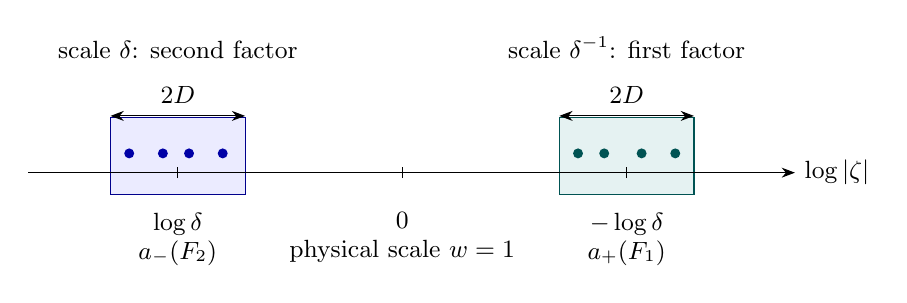
\begin{tikzpicture}[x=.95cm,y=.7cm,>=Stealth,font=\small]
 \fill[blue!8] (-3.9,-.4) rectangle (-2.1,1);
 \fill[teal!10] (2.1,-.4) rectangle (3.9,1);
 \draw[blue!55!black] (-3.9,-.4) rectangle (-2.1,1);
 \draw[teal!65!black] (2.1,-.4) rectangle (3.9,1);
 \draw[->] (-5,0)--(5.25,0) node[right] {$\log|\zeta|$};
 \foreach \x in {-3.65,-3.2,-2.85,-2.4}
   \fill[blue!65!black] (\x,.35) circle (1.8pt);
 \foreach \x in {2.35,2.7,3.2,3.65}
   \fill[teal!65!black] (\x,.35) circle (1.8pt);
 \draw (-3,-.1)--(-3,.1);
 \draw (0,-.1)--(0,.1);
 \draw (3,-.1)--(3,.1);
 \node[below] at (-3,-.55) {$\log\delta$};
 \node[below] at (0,-.55) {$0$};
 \node[below] at (3,-.55) {$-\log\delta$};
 \node[above] at (-3,1.9) {scale $\delta$: second factor};
 \node[above] at (3,1.9) {scale $\delta^{-1}$: first factor};
 \node[below] at (-3,-1.05) {$a_-(F_2)$};
 \node[below] at (0,-1.05) {physical scale $w=1$};
 \node[below] at (3,-1.05) {$a_+(F_1)$};
 \draw[<->] (-3.9,1.03)--(-2.1,1.03)
    node[midway,above=1pt] {$2D$};
 \draw[<->] (2.1,1.03)--(3.9,1.03)
    node[midway,above=1pt] {$2D$};
\end{tikzpicture}

\caption{Schematic zero windows for the two factors: the window at
$\log\delta$ belongs to factor $2$, and the window at $-\log\delta$
belongs to factor $1$. The proof fixes their half-width $D$ and a bound
on the number of zeros before sending $\delta$ to zero. It controls
the state mass of configurations with any zero outside these windows
before expanding at the intervening physical scale $w=1$.}
\label{fig:chiral-windows}
\end{figure}

\begin{proof}
\emph{Spectral functions and exclusion of exterior zeros.}
The strong row actions preceding Lemma~\ref{lem:chiral-representatives}
give convergence of every polynomial in finitely many samples of the two
spectral functions and their complex conjugates. The functions are bounded
by one on the right half-plane; normal-family compactness therefore gives
the joint compact-open convergence. The limiting functions are the original
finite Blaschke spectral functions on the two factors, and are not
identically zero. For a vector $v$, its state spectral measure is
$\sigma_v(B)=\|\bbone_Bv\|^2$ on measurable sets of spectral functions.
These measures have total masses
$\|u_\delta\|^2\to\|u\|^2$; normalization to probability is harmless
when $u\ne0$.

The rescaled quantities in \eqref{eq:chiral-scaled-spectrum} require
control of \emph{every} zero, including zeros between the two scales.
For a fixed core representative, the exterior RTT estimate from
Lemma~\ref{lem:inner-spectra} gives, outside fixed word offsets,
\begin{equation}\label{eq:chiral-exterior-dip}
 \|(I-P(e^s))u_{r_1,r_2}\|^2
      \le C_u\sum_{i=1}^2e^{-2\eta|s-\log r_i|}.
\end{equation}
Every zero $\zeta$ forces a fixed-width interval about $\log|\zeta|$
on which $|1-f(e^s)|$ is bounded below by a positive constant. This
follows from the cone condition and the modulus loss of its single
Blaschke factor; all other factors have modulus at most one.
Integrating \eqref{eq:chiral-exterior-dip} outside slightly smaller
windows thus yields
\begin{equation}\label{eq:chiral-all-zero-event}
\begin{split}
 &\sigma_{u_{r_1,r_2}}
 \left\{\text{some zero lies outside }
     \bigcup_{i=1}^2\{\zeta:|\log(|\zeta|/r_i)|\le D\}\right\}\\
 &\hspace{40mm}\le C_u e^{-c_*D}.
\end{split}
\end{equation}
An additive fixed change in $D$ absorbs the dip width and the word offsets.
To justify the event bound explicitly, if any zero lies outside the enlarged
windows, one entire dip interval lies in the integration region. The
integral of $|1-f(e^s)|^2$ there is then at least a fixed positive number.
Markov's inequality after integration over the state spectral measure gives
\eqref{eq:chiral-all-zero-event}.

\smallskip\noindent
\emph{Complete zero clusters and the physical-scale expansion.}
Here is the order of truncations. Given a desired exceptional mass, first
choose $D$ large enough in \eqref{eq:chiral-all-zero-event} and so that
the finite zero sets of $F_1,F_2$ lie in their annuli with correspondingly
high probability. Choose their boundary circles to carry no limiting zero
almost surely. Only countably many radii are excluded: first restrict to
a bounded zero count, then apply this assertion to its finite intensity
measure, and finally take the union over count bounds. On these fixed
annuli, the cone keeps the zeros in a compact subset of the open right
half-plane. The argument principle and compact-open convergence give joint
convergence of the complete zero multisets, including multiplicities.
Next choose a finite degree bound $M$ so that larger limiting counts have
arbitrarily small mass. Take the scale limit only after $D$ and $M$ have
been fixed. Zero counts and locations now lie in a compact, bounded-count
set, so every product expansion below is uniform. Finally let the allowed
exceptional mass tend to zero, increasing $D$ and $M$ if necessary.

Each limiting product has even degree: conjugate zeros pair, real zeros
contribute a factor $-1$ between the two ends, and both end values are one.
On the preceding high-mass event the complete limiting zero counts occur
in the chosen annuli. Multiplicity convergence therefore makes both
finite-scale clusters even with probability tending to one. This proves
the needed parity; it is not an assumption on a truncated cluster.

For clarity, write the large zeros as $\delta^{-1}\alpha_j$ and the
small zeros as $\delta\beta_j$. On the retained event each normalized
zero has modulus between $e^{-D}$ and $e^D$, and there are at most $M$
zeros. Normalize each factor to one at zero. The two even clusters then
give, for $w=1,i$,
\begin{equation}\label{eq:chiral-product-expansion}
 f(w)=1-\delta\left(
       w\sum_j2\Re\alpha_j^{-1}
          +w^{-1}\sum_j2\Re\beta_j\right)+O_{D,M}(\delta^2).
\end{equation}
The two sums converge jointly to $a_+(F_1)$ and $a_-(F_2)$.
Taking logarithmic modulus at $1$ and phase at $i$ gives
\eqref{eq:chiral-scaled-spectrum}. The middle sign is positive on this
event. Values of $H_0/\delta$ can be arbitrarily large on the discarded
event; convergence in law and bounded multiplier convergence require no
first-moment estimate for that quantity.

\smallskip\noindent
\emph{Strong multiplier convergence and propagators.}
We next strengthen bounded spectral convergence to convergence of vectors.
Choose a countable total word core, including its rational linear
combinations, and exclude the union of the atoms of $A$ in all their state
measures. That union is countable; any other $R$ is admissible in
\eqref{eq:chiral-band-limit}. At such $R$, continuous cutoffs approximate
the indicator in each state $L^2$ norm. More generally, let $b_\delta$ be
a uniformly bounded spectral multiplier with the stated joint limit $b$.
The algebra of polynomials in a countable dense set of interior samples
and their conjugates generates the spectral functions and is dense in
the state $L^2$ space. Given a state $u$, choose such a polynomial $p$ with
$\|(b-p)u\|$ small. Joint convergence gives
\begin{equation}\label{eq:chiral-multiplier-norm}
 \|(b_\delta-p_\delta)u_\delta\|^2
          \longrightarrow\|(b-p)u\|^2.
\end{equation}
For indicators, take the continuous approximations first. Polynomial
actions already converge strongly. Equation
\eqref{eq:chiral-multiplier-norm} proves strong convergence of the
multiplier actions; polarization gives the corresponding mixed pairings.
Lemma~\ref{lem:chiral-representatives} extends these actions to all
strongly converging families and permits their compositions. No assertion
that a current preserves the exceptional-zero event is needed.

Finally, $|f(1)|\le1$ and $|f(i)|=1$. The bounded multipliers
$f(1)^{m_\delta}f(i)^{l_\delta}$ converge jointly by
\eqref{eq:chiral-scaled-spectrum} to
$e^{-xA+iy(-a_+\otimes I+I\otimes a_-)}$, which is
\eqref{eq:chiral-semigroup-limit}. The same vector argument applies.
\end{proof}

The exceptional-event estimate is the reason that local spectral convergence
can be used at the intervening physical scale $w=1$. It also permits the
energy cutoffs needed for current insertions. We next prove their convergence
in norm, before removing those cutoffs by time damping.

\subsection{Current insertions and damping}

\begin{lemma}\label{lem:current-limit}
For every admissible $R>0$ in Proposition~\ref{prop:two-scale} and every
$|w|=1$ with $\Re w\ge0$,
\begin{equation}\label{eq:chiral-current-limit}
 \delta^{-1}Q_\delta(R)N(w)Q_\delta(R)
 \longrightarrow
 Q(R)\bigl(w(j_+\otimes I)+w^{-1}(I\otimes j_-)\bigr)Q(R)
\end{equation}
strongly on representatives. All displayed operators are bounded at fixed
$R$. Finite products with propagators from
\eqref{eq:chiral-semigroup-limit} converge when successive positive time
gaps stay bounded below. In these vacuum products, the cutoffs on both
sides of each current may be removed after the scale limit, with error
tending to zero uniformly on compact sets of separated time coordinates.
\end{lemma}

\begin{proof}
Write $Q_\delta=Q_\delta(R)$ and $Q=Q(R)$. Glue
$J_\delta(w)=Q_\delta J(w)Q_\delta$ to the full annulus
\[
                  CR\delta<|w|<c_* /(R\delta)
\]
using Lemma~\ref{lem:low-band}. Let $C_{k,\delta}$ be its Laurent
coefficients. Fix $\rho>0$ sufficiently small compared with $R^{-1}$.
At the outer circle, the substitution $v=\delta w$ gives
\begin{equation}\label{eq:chiral-outer-coefficient}
 \delta^{-1}C_{1,\delta}
    =\frac1{2\pi i}\int_{|v|=\rho}
                  J_\delta(v/\delta)\frac{dv}{v^2}.
\end{equation}
At the inner circle, put $w=\delta v$ to obtain
\begin{equation}\label{eq:chiral-inner-coefficient}
 \delta^{-1}C_{-1,\delta}
    =\frac1{2\pi i}\int_{|v|=\rho^{-1}}
                              J_\delta(\delta v)\,dv.
\end{equation}
Both contours are counterclockwise. The rescaled contours are fixed, and
both integrands are uniformly bounded in operator norm at fixed $R,\rho$.

On the strict right semicircle the marked rows converge on their respective
tensor factors. The cutoffs converge strongly by
\eqref{eq:chiral-band-limit}. On the reflected semicircle the integrand is
the product specified by reversal, for example
\[
 -\bigl(Q_\delta P(v/\delta)^{-1}Q_\delta\bigr)
     J_\delta(v/\delta)
     \bigl(Q_\delta P(v/\delta)^{-1}Q_\delta\bigr).
\]
The inverse factors are uniformly bounded spectral multipliers on
$Q_\delta\mathcal D$ only. Their joint limits follow from
Proposition~\ref{prop:two-scale}, since on $Q\mathcal D^{\otimes2}$
the first energy is at most $R$ and \eqref{eq:chiral-disc-inverse}
applies. The second contour uses the analogous estimate at infinity.
Lemma~\ref{lem:chiral-representatives} therefore proves convergence of
these noncommuting products at every strict contour point.

Here is the norm justification for passing through the contour integrals.
For a representative $u_\delta$, let $v_\delta(t)$ be the integrand
applied to it, including the scalar contour weight, and let $v(t)$ be
its limit. The vectors are bounded uniformly in $t,\delta$. Core test
pairings of $\int v_\delta(t)dt$ converge by a single dominated integral.
Their squared norms converge because
\begin{equation}\label{eq:chiral-double-contour}
 \left\|\int v_\delta(t)dt\right\|^2
 =\iint\langle v_\delta(t),v_\delta(s)\rangle\,dt\,ds
 \longrightarrow
 \iint\langle v(t),v(s)\rangle\,dt\,ds.
\end{equation}
Pairings of strongly convergent representatives converge, so dominated
convergence applies to this double integral. The two imaginary-axis points
have contour measure zero. The norm criterion in
Lemma~\ref{lem:chiral-representatives} now gives strong convergence of
each coefficient action. By the definitions of the chiral forms, the
limits of \eqref{eq:chiral-outer-coefficient} and
\eqref{eq:chiral-inner-coefficient} are respectively
\[
                 Q(j_+\otimes I)Q,
                   \qquad Q(I\otimes j_-)Q.
\]

It remains to pass from these coefficients to $N$. Put
$\Sigma=\sgn P(1)$ and
\[
 T_\delta(w)=w\delta^{-1}C_{1,\delta}
                         +w^{-1}\delta^{-1}C_{-1,\delta}.
\]
The same-sign and opposite-sign estimates of Lemma~\ref{lem:low-band}
give, for some $\theta>0$,
\begin{equation}\label{eq:chiral-sign-removal}
 \delta^{-1}Q_\delta N(w)Q_\delta
       =\tfrac12\bigl(\Sigma T_\delta(w)+T_\delta(w)\Sigma\bigr)
                       +O_R(\delta^\theta)
\end{equation}
in operator norm, uniformly on the unit semicircle. Indeed the
anticommutator is $+T_\delta$ on the positive-sign block,
$-T_\delta$ on the negative-sign block, and zero between opposite signs.
On same-sign blocks the even Laurent part and all odd modes of order
larger than one vanish after rescaling, with the stated remainder.
The opposite-sign block of the rescaled $N$ has the same vanishing bound.
Proposition~\ref{prop:two-scale} gives $\Sigma\to I$ strongly on
representatives. The coefficient operators are uniformly bounded and have
the strong limits just proved. Composition in
\eqref{eq:chiral-sign-removal} proves \eqref{eq:chiral-current-limit}.
The low-band bounds include the endpoints $w=\pm i$.

We finish with a summable bound for removing cutoffs. For all $U>0$ and
all sufficiently small $\delta$,
\begin{equation}\label{eq:chiral-all-band-bound}
 \|\bbone_{H_0/\delta\le U}\,\delta^{-1}N(w)
                      \bbone_{H_0/\delta\le U}\|\le CU.
\end{equation}
If $U\delta$ is small this is Lemma~\ref{lem:low-band}; otherwise the
global bound on $N$ gives it by $\delta^{-1}\le C U$.
Decompose $H_0/\delta$ into bands $[0,1]$ and
$(2^{q-1},2^q]$, $q\ge1$. A current block between levels $q,r$ costs
at most $C\max(2^q,2^r)$. Each internal propagator with
$\delta m\ge b>0$ supplies at level $q\ge1$ the factor
$e^{-b2^{q-1}}$, since
$\|P(1)^m\bbone_{H_0/\delta>2^{q-1}}\|\le e^{-b2^{q-1}}$;
unit shifts do not affect this norm.
The outer states are the vacuum, of energy zero. For a product of $k$
currents, a bound for the sum over its $k-1$ internal indices is a constant
times
\begin{equation}\label{eq:chiral-dyadic-majorant}
 \sum_{q_1,\ldots,q_{k-1}\ge0}
       \prod_{j=1}^{k-1}(1+2^{q_j})^2e^{-b'2^{q_j}},
                         \qquad b'>0.
\end{equation}
This converges, and its tails with any $2^{q_j}>R$ tend to zero uniformly
in the mesh. The limiting forms have the identical bound using $A$ and
\eqref{eq:chiral-form-bound}. Fixed-cutoff convergence, followed by this
tail estimate, proves the product assertion. The constants are uniform
when the finitely many limiting time gaps have a fixed positive lower
bound.
\end{proof}

\subsection{The limiting derivative correlations}

For the centered differences introduced at the start of the section,
Lemma~\ref{lem:current-limit} and
\eqref{eq:chiral-semigroup-limit} show that the insertions of
$\delta^{-1}D_\delta^+$ and $\delta^{-1}D_\delta^-$ converge to
$-j_+\otimes I$ and $-I\otimes j_-$, respectively. For example,
the two combinations follow from
\[
 N(1)\rightsquigarrow j_+\otimes I+I\otimes j_-,
 \qquad
 N(i)\rightsquigarrow i j_+\otimes I-i I\otimes j_-.
\]
Currents in different factors commute. Their propagators and the tensor
vacuum factor as well. The limiting mixed correlations therefore factor
into a pure $+$ correlation and a pure $-$ correlation.

Write $a=a_+$ and $j=j_+$ for the moment. For increasing real parts,
$\Re z_{i_1}<\cdots<\Re z_{i_k}$, define
\begin{equation}\label{eq:chiral-ordered-function}
 F_k(z_1,\ldots,z_k)
 =\left\langle\Omega,\,
 (-j)e^{-(z_{i_k}-z_{i_{k-1}})a}(-j)\cdots
 e^{-(z_{i_2}-z_{i_1})a}(-j)\Omega\right\rangle.
\end{equation}
Set $F_0=1$ and $F_1=0$. The products in
\eqref{eq:chiral-ordered-function} are defined by inserting positive
real damping on both sides of each form; arbitrary extra end damping
may be inserted because $a\Omega=0$. Lemma~\ref{lem:chiral-forms}
makes the resulting factors bounded, and the dyadic tail bound shows
that the value is independent of this allocation. By reality of the
height field, the pure $-$ answer is $\overline{F_k(z_1,\ldots,z_k)}$.
All the preceding convergence is uniform on compact subsets of the
region of distinct real coordinates. Indeed, it holds along every
sequence of moving mesh faces converging to such a configuration,
and the cutoff and damping bounds are uniform on its compact subsets.

The two-point function is already explicit. If $\Re z_1<\Re z_2$,
skew-adjointness, the vacuum identity and
\eqref{eq:chiral-Haar-integral} give
\[
 F_2(z_1,z_2)
 =-\int a(f)^2e^{-(z_2-z_1)a(f)}\,d\mu(f)
 =-\kappa\int_0^\infty t e^{-(z_2-z_1)t}\,dt
 =-\frac{\kappa}{(z_2-z_1)^2}.
\]
The integrals converge because $\Re(z_2-z_1)>0$.
For higher moments, we need this coefficient at a collision even between
nonvacuum exterior states.

We now determine these holomorphic correlations from their singularities.
The two axial orderings give analytic formulas away from a finite grid of
possible punctures. We will bound the growth at every puncture, compute the
coefficient when two physical points actually collide, and remove the
remaining artificial punctures. These facts and decay at infinity will
force Wick's recursion.

\begin{lemma}\label{lem:chiral-holomorphy}
Let
\[
 U_x=\{(z_1,\ldots,z_k):\Re z_i\ne\Re z_j\text{ for }i\ne j\},
 \quad
 U_y=\{(z_1,\ldots,z_k):\Im z_i\ne\Im z_j\text{ for }i\ne j\}.
\]
The function $F_k$ has a symmetric, jointly holomorphic extension to
$U_x\cup U_y$, and is the limit of the centered $+$ derivative
correlations on both sets.

Fix $z_2,\ldots,z_k$ with distinct real coordinates and distinct imaginary
coordinates. As a function of $z_1$, the extension is holomorphic away
from the grid points
\begin{equation}\label{eq:chiral-grid-points}
                    p_{jh}=\Re z_j+i\Im z_h,\qquad 2\le j,h\le k.
\end{equation}
Near any such point it is $O(|z_1-p_{jh}|^{-2})$, locally uniformly
as the fixed points vary while retaining these coordinate separations.
For $k\ge2$ it tends to zero as $|z_1|\to\infty$ with the other points fixed.
\end{lemma}

\begin{proof}
On a compact subset of an eastward ordering chamber, give each current
a fixed positive amount of damping on both sides. The remaining
semigroups have parameters with real parts bounded below. These
semigroups are holomorphic in operator norm there: for instance
$\|a^m e^{-sa}\|\le m!s^{-m}$ after reducing $s$ by a fixed factor.
The resulting bounded product is jointly holomorphic in all its
parameters. This proves joint holomorphy on $U_x$, rather than merely
separate holomorphy.

By Proposition~\ref{prop:physical-plane}, northward quantization describes
the same physical law. In its coordinates $z'=-iz$, the centered
differences transform as
$D_{x',\delta}=D_{y,\delta}$ and
$D_{y',\delta}=-D_{x,\delta}$, hence
$D_\delta^+=-iD_\delta^{\prime+}$. The possible face-origin shift is
one lattice spacing and is covered by moving-face convergence. The
northward formula is thus holomorphic on $U_y$. On $U_x\cap U_y$
both formulas are limits of the same physical moments, so they agree
and glue. Permuting the insertions does not change a physical product,
which proves symmetry.

With the other points as in the statement, failure of both axial
orderings occurs only at the grid points \eqref{eq:chiral-grid-points}.
Choose a small neighborhood of the fixed configuration in which all
its real gaps and imaginary gaps remain at least $b>0$. Near $p_{jh}$,
the eastward representation has only one possibly small gap,
$g_x=|\Re(z_1-p_{jh})|$, between $z_1$ and $z_j$.
The northward representation has only one possibly small gap,
$g_y=|\Im(z_1-p_{jh})|$, between $z_1$ and $z_h$.
Use the ordering with $g=\max(g_x,g_y)\ge|z_1-p_{jh}|/\sqrt2$.
Only the two currents bordering that gap need shrinking damping.
Give each damping $g/4$ on both sides: the inner dampings consume
$g/2$, and the outer dampings come from neighboring fixed gaps or
from a vacuum endpoint. All other currents receive fixed damping.
Equation~\eqref{eq:chiral-damped-form} gives a cost $C/g$ for each
of the two currents and a bounded cost for the rest. This proves
the uniform quadratic bound. A point sharing the other coordinate
is separated in the chosen ordering.

Finally, when $|z_1|$ is large, one coordinate makes $z_1$ extreme in
the corresponding ordering, with a gap $g$ of order $|z_1|$ to all
other points. Give the isolated current damping of order $g$ on both
sides, using free damping on its vacuum side. Keep fixed damping
around all remaining currents. The isolated factor costs $C/g$;
imaginary semigroup factors have norm one. Thus $F_k\to0$ at infinity.
\end{proof}

\subsection{The collision operator}

The remaining input for Gaussianity is the coefficient at a genuine
collision. A second separation of scales shows that a short pair of
chiral currents becomes a scalar, even between nonvacuum exterior states.

\begin{lemma}\label{lem:collision}
For $a=a_+$ and $j=j_+$, the bounded operators
\begin{equation}\label{eq:chiral-collision-operator}
 K_\epsilon=e^{-\epsilon a}(\epsilon j)e^{-\epsilon a}
                      (\epsilon j)e^{-\epsilon a}
\end{equation}
are uniformly bounded for $\epsilon>0$ and satisfy
\begin{equation}\label{eq:chiral-collision-limit}
                    K_\epsilon\rightharpoonup-\kappa I
                       \qquad(\epsilon\downarrow0).
\end{equation}
Consequently, fix $z_2,\ldots,z_k$ with pairwise distinct real
coordinates and pairwise distinct imaginary coordinates, and let
$2\le j\le k$. Then
\begin{equation}\label{eq:chiral-double-pole}
 \lim_{\epsilon\downarrow0}\epsilon^2
 F_k(z_j+\epsilon,z_2,\ldots,z_k)
   =-\kappa F_{k-2}(z_2,\ldots,\widehat z_j,\ldots,z_k).
\end{equation}
The coefficient on the right is independent of both colliding positions.
\end{lemma}

\begin{proof}
Split the middle damping of \eqref{eq:chiral-collision-operator} into
two halves. Each of the resulting damped current factors has norm bounded
by a constant, by \eqref{eq:chiral-damped-form} at scale $\epsilon/2$.
This gives uniform boundedness.

Apply the representative construction with scales $r_1=\epsilon$ and
$r_2=1$. Its Gram and row limits use only separation of the two scales,
so they are unchanged. The all-zero event estimate
\eqref{eq:chiral-all-zero-event}, with the same order of fixed windows,
bounded degree, and then scale limit, gives
\begin{equation}\label{eq:chiral-collision-energy}
                     \epsilon a(f)\longrightarrow a(F_1)
\end{equation}
jointly with the two spectral functions. To see the scaling directly,
a zero $\epsilon\alpha$ contributes $2\Re\alpha^{-1}$ to $\epsilon a$,
whereas a zero $\beta$ at the unshifted scale contributes
$2\epsilon\Re\beta^{-1}$. On the bounded-count annuli the latter
sum tends uniformly to zero. The exceptional-zero event has arbitrarily
small mass and is discarded before making this expansion.

Choose a non-atomic band endpoint and put
$B_\epsilon=\bbone_{\epsilon a\le R}$ and
$B=\bbone_{a\otimes I\le R}$. The spectral multiplier argument proves
$B_\epsilon\to B$ strongly. The definition of $j$ by its Taylor
coefficient gives, for a sufficiently small fixed $\rho<c_*/R$,
\begin{equation}\label{eq:chiral-collision-contour}
 \epsilon B_\epsilon jB_\epsilon
   =\frac1{2\pi i}\int_{|v|=\rho}
             B_\epsilon J(\epsilon v)B_\epsilon\,\frac{dv}{v^2}
   \longrightarrow B(j\otimes I)B.
\end{equation}
Indeed, the unscaled band is $a\le R/\epsilon$, whose Taylor disc
has radius proportional to $\epsilon/R$. On the right semicircle
the row acts on the first factor; on the left semicircle the bounded
compressed inverse and reversal apply. The single- and double-contour
argument \eqref{eq:chiral-double-contour} proves convergence in
representative norm. Thus \eqref{eq:chiral-collision-energy} and
\eqref{eq:chiral-collision-contour} give the cutoff limit of
$K_\epsilon$.

These cutoffs can be removed in operator norm uniformly in $\epsilon$.
Decompose $\epsilon a$ into $[0,1]$ and the dyadic bands above one.
A block of $\epsilon j$ between levels $q,r$ costs at most
$C\max(2^q,2^r)$. The three damping factors of $K_\epsilon$ give an
absolutely summable majorant
\[
 C\sum_{q_0,q_1,q_2\ge0}
   \max(2^{q_0},2^{q_1})\max(2^{q_1},2^{q_2})
                       e^{-b(2^{q_0}+2^{q_1}+2^{q_2})}.
\]
Absorbing the lowest-band constants into $C$ gives some fixed $b>0$.
The part with any $2^{q_i}>R$ tends to zero as $R\to\infty$.
The same estimate holds for the limiting tensor product. Therefore,
on separated-scale representatives,
\[
 K_\epsilon\longrightarrow
           \bigl(e^{-a}je^{-a}je^{-a}\bigr)\otimes I.
\]

A fixed unboosted word vector $u$ is exactly the representative of
$\Omega\otimes u$: its small-scale word is the identity. Hence for
fixed word vectors $u,v$ the last limit contracts the first factor to
\[
 \langle\Omega,je^{-a}j\Omega\rangle
   =-\int a(f)^2e^{-a(f)}\dd\mu(f)
   =-\kappa\int_0^\infty t e^{-t}\,dt=-\kappa.
\]
The sign uses the skew-adjointness of $j$; the integrals are justified
by \eqref{eq:chiral-Haar-integral}. This proves
\eqref{eq:chiral-collision-limit} on a dense set of test vectors.
Uniform boundedness extends it to every pair of vectors in $\mathcal D$.

For \eqref{eq:chiral-double-pole}, take $z_1=z_j+\epsilon$ in the
eastward ordering. The two colliding currents are consecutive. After
multiplication by $\epsilon^2$, their part of the product becomes
$K_\epsilon$, provided its two outer dampings are subtracted from the
adjacent exterior gaps. Those gaps remain positive for small $\epsilon$;
at an endpoint, insert damping freely on the vacuum. The two exterior
vectors converge strongly, because all their damping gaps remain positive.
They may therefore be replaced by their limits in the weak convergence
of the uniformly bounded $K_\epsilon$. The two insertion minus signs
cancel. Omitting the colliding currents recombines the adjoining
semigroups, giving exactly the right side of
\eqref{eq:chiral-double-pole}. No dependence on the collision position
remains.
\end{proof}

\subsection{Removal of artificial poles and Wick recursion}

\begin{proposition}\label{prop:gaussian-currents}
Let $k\ge1$, and let $z_1,\ldots,z_k$ have pairwise distinct real
coordinates or pairwise distinct imaginary coordinates. For
$\varepsilon_i\in\{+,-\}$ and moving mesh faces $z_{i,\delta}\to z_i$,
\begin{equation}\label{eq:chiral-Gaussian-current-limit}
 \lim_{\delta\downarrow0}
 \E\prod_{i=1}^k
       \delta^{-1}D_\delta^{\varepsilon_i}h_\delta(z_{i,\delta})
   =\sum_{\pi}\ \prod_{\{i,j\}\in\pi}
                  C_{\varepsilon_i,\varepsilon_j}(z_i,z_j),
\end{equation}
where the sum is over pairings, is zero for odd $k$, and
\begin{equation}\label{eq:chiral-contractions}
 C_{++}(z,\xi)=-\frac{\kappa}{(z-\xi)^2},\qquad
 C_{--}(z,\xi)=-\frac{\kappa}{(\bar z-\bar\xi)^2},\qquad
 C_{+-}(z,\xi)=C_{-+}(z,\xi)=0.
\end{equation}
Convergence is uniform on compact subsets of either separated-time
region. By linearity the corresponding assertion holds for all products
of the real centered derivatives $\delta^{-1}D_{x,\delta}$ and
$\delta^{-1}D_{y,\delta}$. These are the off-diagonal derivatives of the
Gaussian covariance
\begin{equation}\label{eq:chiral-log-covariance}
                              K_\kappa(z,\xi)=-2\kappa\log|z-\xi|.
\end{equation}
\end{proposition}

\begin{proof}
The preceding lemmas already give the limits as products of pure chiral
functions and their conjugates. It remains to determine $F_k$.
Fix generic spectators $z_2,\ldots,z_k$ as in
Lemma~\ref{lem:chiral-holomorphy}. Its quadratic bound makes every
grid puncture of $F_k$ a pole of order at most two: the Cauchy bound
for a Laurent coefficient of order $-m$, $m>2$, is $Cr^{m-2}$ on a
circle of radius $r$, and tends to zero.

First consider an artificial puncture
$p=p_{jh}=\Re z_j+i\Im z_h$ with $j\ne h$.
Take a fixed small circle $\Gamma$ about its position for the chosen
spectators. In a sufficiently small complex neighborhood of the
spectators, the circle encloses just this moving grid point and remains
in $U_x\cup U_y$. The contour moments
\[
 m_\ell=\frac1{2\pi i}\int_\Gamma
                  \zeta^\ell F_k(\zeta,z_2,\ldots,z_k)\,d\zeta
\]
are jointly holomorphic in the spectator variables, by the uniform
bounds and joint holomorphy on the circle. If the principal part is
$A/(\zeta-p)^2+B/(\zeta-p)$, residue calculation gives
\begin{equation}\label{eq:chiral-pole-moments}
 m_\ell=Bp^\ell+A\ell p^{\ell-1},\qquad
 m_0m_2-m_1^2=-A^2,\qquad
 m_0m_3-m_1m_2=-2pA^2.
\end{equation}
If $A$ is nonzero at any parameter value, the nonzero denominator
persists locally and
\[
             p=\frac{m_0m_3-m_1m_2}
                       {2(m_0m_2-m_1^2)}
\]
is holomorphic there. This is impossible, since
\[
 p=\frac{z_j+\bar z_j}{2}+\frac{z_h-\bar z_h}{2},
                         \qquad \partial_{\bar z_j}p=\tfrac12.
\]
Thus $A$ vanishes. If $B$ is nonzero, $p=m_1/m_0$ gives the same
contradiction. Every artificial puncture is removable.
This removal is joint in the parameters: inside $\Gamma$, the Cauchy
integral of $F_k(\eta,\mathbf z)/(\eta-\zeta)$ supplies a jointly
holomorphic extension and agrees with each one-variable removable
extension.

At a true collision, put
$\xi=(z_1+z_j)/2$ and $d=z_1-z_j$, retaining generic exterior points.
Locally the union $U_x\cup U_y$ contains every $d\ne0$.
The function
$H(\xi,d,\mathbf z)=d^2F_k$ is uniformly bounded there and therefore
extends jointly holomorphically to $d=0$. One can see this directly
by its Cauchy coefficients in $d$: boundedness removes the negative
coefficients, uniformly on smaller spectator neighborhoods.
Symmetry under exchanging the two colliding insertions makes $H$ even
in $d$. Lemma~\ref{lem:collision} identifies its constant term as
\[
 H(\xi,0,\mathbf z)
             =-\kappa F_{k-2}(\mathbf z),
\]
independent of $\xi$. Subtracting this term leaves an even holomorphic
function with zero constant term, hence a function divisible by $d^2$.
It follows that
\[
 F_k+\frac{\kappa F_{k-2}(\mathbf z)}{(z_1-z_j)^2}
\]
is holomorphic at this diagonal. In particular there is no simple
residue. Independence of the collision center is needed here: a varying
coefficient of $d^{-2}$ could otherwise create a simple term when
$z_j$ is held fixed.

Subtract all these true double-pole terms as a function of $z_1$.
The artificial points are removable, the true points have no remaining
principal parts, and the resulting function is entire.
Lemma~\ref{lem:chiral-holomorphy} gives decay at infinity, and the
subtracted rational terms also decay there. Liouville's theorem yields
\begin{equation}\label{eq:chiral-Wick-recursion}
 F_k(z_1,\ldots,z_k)
   =-\kappa\sum_{j=2}^k
       \frac{F_{k-2}(z_2,\ldots,\widehat z_j,\ldots,z_k)}
                           {(z_1-z_j)^2}.
\end{equation}
Together with $F_0=1$ and $F_1=0$, this is Wick's recursion with
contraction $-\kappa/(z_i-z_j)^2$. Continuity extends it from the
generic spectators to every strict axial chamber. Factorization of
the two chiral sectors and reality then give
\eqref{eq:chiral-Gaussian-current-limit}.

Finally,
$\partial_z\partial_\xi K_\kappa(z,\xi)=-\kappa/(z-\xi)^2$ and
$\partial_z\partial_{\bar\xi}K_\kappa(z,\xi)=0$ away from collisions.
The conjugate identity gives the other pure contraction. This proves
the covariance assertion and, by linearity, all the real derivative
formulas. The uniform moving-face convergence established above gives
the asserted local uniformity. Estimates across a time-ordering wall
and for undifferentiated fields will be supplied in
Section~\ref{sec:probability}; none is needed for this proposition.
\end{proof}

\section{Moment bounds and convergence of the height field}\label{sec:probability}

The current limits of Section~\ref{sec:chiral} concern insertions at
separated times. We now pass to the height field itself. We first identify its law on smooth neutral tests, then remove endpoint
smoothings to obtain the separated increment moments. The logarithmic
variogram bound extends this identification to finite-energy signed
measures. After these three steps, we prove tightness in negative
regularity, treating ordinary restriction spaces, the outward test
convention, and intrinsic dual spaces separately.

Two estimates drive these passages. An energy-commutator argument gives
uniform ordinary moments for neutral spatial averages. A small neutral
factor separated from all other factors has a correlation that tends to
zero as a positive power of its diameter. The latter estimate makes the
successive removal of endpoint smoothings summable.

Throughout the angular argument, fix \(0<c<2\), and retain the plane state,
\(\kappa\), the vacuum \(\Omega\), the shift \(S=P(i)\), and the
nonnegative endpoint Hamiltonian \(E\) from Section~\ref{sec:angular}.
The Gaussian field appearing before its normalization is identified has
covariance
\begin{equation}\label{eq:prob-log-kernel}
 K_\kappa(x,y)=-2\kappa\log|x-y|.
\end{equation}
We denote this field modulo constants by \(\mathcal H_\kappa\).
All constants below may depend on the fixed parameter and the stated
moment order. None depends on an integer approximation to \(\delta^{-1}\):
\(\delta>0\) is always an arbitrary real mesh size.

\subsection{Ordinary moments from the endpoint Hamiltonian}

On an equal-time column, \(Z_l\) is the diagonal spin at site \(l\), with
values \(\pm1\). These are self-adjoint site operators; they should be
distinguished from marked time rows. A path height increment is the
negative of its step spin. Vacuum moments of the commuting site spins
are their ordinary moments under \(\P_c\).

\begin{lemma}[Ordinary spatial moments]\label{lem:ordinary-moments}
Fix \(0<A<\infty\). Let \(R\ge1\), and let \(g=(g_l)_{l\in\Z}\) be a
finitely supported real sequence such that
\begin{equation}\label{eq:prob-g-conditions}
 \sum_l|g_l|\le AR,\qquad
 \sum_l|g_{l+1}-g_l|\le A,\qquad
 \sum_l|g_{l+1}-g_l|^2\le A/R.
\end{equation}
Then, for every \(1\le b<\infty\),
\begin{equation}\label{eq:prob-ordinary-moments}
 \left\|\sum_lg_lZ_l\right\|_{L^b(\P_c)}\le C_{A,b}.
\end{equation}
In particular the conclusion holds if \(g\) has support of length at
most \(AR\), \(|g_l|\le A\), and
\(|g_{l+1}-g_l|\le A/R\). The same assertions hold with the two axes
interchanged.
\end{lemma}

\begin{proof}
Work throughout this proof in \(\mathcal H_{\mathrm{spin}}\), the closed
span of \(O\Omega\) with \(O\) a finite local spin matrix.
By Lemma~\ref{lem:endpoint-Hamiltonian}, this subspace contains
\(\Omega\) and reduces \(E\). Every finite local spin matrix and its
adjoint preserve the local generating vectors and hence their closed
span. In particular \(D=D_g=\sum_lg_lZ_l\) is bounded and self-adjoint
on \(\mathcal H_{\mathrm{spin}}\). The shift preserves this subspace
in both directions, since it translates local matrices and fixes
\(\Omega\). In this proof \(E\) denotes its self-adjoint restriction
to \(\mathcal H_{\mathrm{spin}}\),
\(B_M=\bbone_{\{E\le M/R\}}\) is its spectral projection there, and
all Hilbert-space norms are taken on this subspace.

First we prove a two-sided compression bound. For fixed \(M\),
Lemma~\ref{lem:endpoint-Hamiltonian} places the range of \(B_M\)
inside the ambient spectral band \(H_0\le C M/R\), when \(R\) is
sufficiently large. The full-space estimates of Lemma~\ref{lem:low-band}
therefore apply to these compressions without increasing their norms.
The identity
\[
 N(i)=\tfrac12S^2(Z_0+Z_1)
\]
and translation by the unitary shift therefore give
\(\|B_M(Z_l+Z_{l+1})B_M\|\le C_M/R\).
Pair the consecutive sites in the sum for \(D\). The coefficients of the
paired sums have total absolute value at most \(AR\); the remaining
single-site terms have total absolute coefficient at most
\(\sum_l|g_{l+1}-g_l|\). Consequently
\begin{equation}\label{eq:prob-two-sided}
 \|B_MDB_M\|\le C_{A,M}.
\end{equation}
For bounded \(R\), this follows instead from
\(\|D\|\le\sum_l|g_l|\).

The local-link description of \(E\) in
Lemma~\ref{lem:endpoint-Hamiltonian} gives
\begin{equation}\label{eq:prob-double-commutator}
 \|[D,[E,D]]\|\le C\sum_l|g_{l+1}-g_l|^2\le C_A/R.
\end{equation}
Indeed the diagonal part of a link commutes with \(D\), and its spin
exchange preserves \(Z_l+Z_{l+1}\); only the coefficient difference
\(g_l-g_{l+1}\) enters each commutator. These identities initially hold
on the local analytic core in \(\mathcal H_{\mathrm{spin}}\), which is
a core for the restricted \(E\). On that core, \([E,D]\) is a finite
sum of bounded local operators. To extend it, approximate a vector in
\(\Dom(E)\subset\mathcal H_{\mathrm{spin}}\) in the graph norm by local
core vectors and use \(EDu=DEu+[E,D]u\) there. Boundedness of \(D\)
and of this commutator, followed by closedness of \(E\), shows that
\(D\) preserves the restricted domain and that the identity extends to
it. The same holds for every fixed local power of \(D\), justifying
the following energy-projection and vacuum calculations on this subspace.

Set \(m_* =\|DB_1\|\), which is finite since \(D\) is bounded.
For a unit vector \(u\in B_1\mathcal H_{\mathrm{spin}}\), expanding the double
commutator yields
\[
 \langle Du,EDu\rangle
 =\tfrac12\langle u,[D,[E,D]]u\rangle
      +\Re\langle Du,DEu\rangle
 \le \frac{C_A+m_*^2}{R}.
\]
Here \(Eu\in B_1\mathcal H_{\mathrm{spin}}\) and \(\|Eu\|\le R^{-1}\).
The component of \(Du\) above energy \(2/R\) thus has squared norm at
most \((C_A+m_*^2)/2\). Its component below \(2/R\) is bounded by
\eqref{eq:prob-two-sided}, with \(M=2\). Taking a supremum gives
\[
 m_*^2\le C_A+\tfrac12m_*^2,
 \qquad\text{and therefore}\qquad
 \|DB_1\|=\|B_1D\|\le C_A.
\]

We next bound powers of \(D\) on the vacuum. Since \(E\Omega=0\),
\[
 2\langle D^k\Omega,ED^k\Omega\rangle
 =\langle\Omega,[D^k,[E,D^k]]\Omega\rangle.
\]
In the site-diagonal representation, let \(D^{\mathrm{sw},l}\) be the
value of \(D\) after exchanging the spins at \(l,l+1\). An exchange
term in this double commutator has, up to a bounded link coefficient
and sign, the multiplier
\(\bigl(D^k-(D^{\mathrm{sw},l})^k\bigr)^2\).
This nonnegative multiplier commutes with the exchange. Furthermore,
\[
 |D-D^{\mathrm{sw},l}|\le2|g_l-g_{l+1}|,
 \qquad
 \bigl|D^k-(D^{\mathrm{sw},l})^k\bigr|^2
 \le C_{A,k}|g_l-g_{l+1}|^2(1+|D|^{2k-2}).
\]
For the second inequality use the factorization of \(a^k-b^k\) and
\(|a-b|\le2A\). Taking the absolute value of an exchange expectation
is bounded by the expectation of its nonnegative multiplier, since the
exchange is a norm-one involution commuting with that multiplier.
Summing the links proves
\begin{equation}\label{eq:prob-power-energy}
 \langle D^k\Omega,ED^k\Omega\rangle
 \le \frac{C_{A,k}}R
       \bigl(1+\|D^{k-1}\Omega\|^2\bigr).
\end{equation}
The low-energy component satisfies
\(\|B_1D^k\Omega\|\le C_A\|D^{k-1}\Omega\|\); on its complement,
positivity of \(E-R^{-1}\) bounds the squared norm by
\(R\langle D^k\Omega,ED^k\Omega\rangle\).
Induction in \(k\) now bounds every \(\|D^k\Omega\|\).
These are the even ordinary moments of \(D\); interpolation gives all
finite orders. Axial symmetry gives the other orientation.
\end{proof}

\begin{corollary}[Neutral blocks]\label{cor:neutral-blocks}
Let \(b\in\R^2\), \(r>0\), and let \(f\) be a measurable real density
supported in a square of side \(Ar\) centered within distance \(Ar\)
of \(b\), with
\[
 \int f=0,\qquad |f|\le A r^{-2}.
\]
For every finite \(q\),
\begin{equation}\label{eq:prob-neutral-block}
 \|\langle h_\delta,f\rangle\|_{L^q}\le C_{A,q}
\end{equation}
uniformly in \(b,r,\delta\). Products of finitely many such blocks have
uniform absolute moment bounds, even when their supports overlap.
\end{corollary}

\begin{proof}
Suppose first \(r/\delta\ge1\), and put \(R=r/\delta\).
Integrate \(f\) on mesh cells, giving masses \(a_{jl}\) of size
\(O(R^{-2})\), with \(O(R)\) possible indices in each direction.
Let \(m_j=\sum_l a_{jl}\), and choose a mass-one discrete profile
\((p_l)\), of width \(O(R)\), bounded by \(C/R\).
The masses \(a_{jl}-m_jp_l\) are neutral in each column. Their discrete
primitives are bounded by \(C/R\), with consecutive differences
\(O(R^{-2})\). Summation by parts and
Lemma~\ref{lem:ordinary-moments}, applied after multiplication by \(R\),
bound the \(L^q\) norm of each column contribution by \(C_q/R\).
Their sum is bounded by Minkowski's inequality.
For the remaining masses \(m_jp_l\), note that
\(\sum_jm_j=0\), \(|m_j|\le C/R\); sum by parts in the other axis,
then average against \(p_l\). This gives the same bound.
If \(r<\delta\), the support meets only a bounded number of neighboring
faces. Neutrality, bounded total variation, and unit height jumps give
a deterministic bound. Finally apply Hölder's inequality to products,
using the required higher moments. No disjointness is used.
\end{proof}

\subsection{Smooth test functions}

\begin{proposition}\label{prop:smooth-tests}
For every finite family of smooth compactly supported densities
\(\phi_1,\ldots,\phi_m\) of integral zero, the vector
\(\bigl(\langle h_\delta,\phi_i\rangle\bigr)_i\) converges jointly in law
and in every joint moment to the corresponding pairings of
\(\mathcal H_\kappa\). The moment convergence is uniform when the tests
vary in a compact smooth family with a common compact support.
\end{proposition}

\begin{proof}
First assume that \(\int\phi(x,y)\,dy=0\) for every \(x\).
For fixed continuum time \(x\), put
\(F(x,y)=\int_{-\infty}^y\phi(x,t)\,dt\).
Discrete summation by parts writes the line pairing as
\[
 \int h_\delta(x,y)\phi(x,y)\,dy
 =-\sum_{l\in\Z}F(x,(l+1)\delta)
       \bigl(h(\lfloor x/\delta\rfloor,l+1)
             -h(\lfloor x/\delta\rfloor,l)\bigr).
\]
The primitive is compactly supported, bounded, and changes by \(O(\delta)\)
at consecutive sites. Lemma~\ref{lem:ordinary-moments} therefore bounds
this pairing in every \(L^q\), uniformly in \(x\) and \(\delta\).
The same remains true for any finite product of line pairings.

Replace the forward height differences in this expression by the
centered differences of Proposition~\ref{prop:gaussian-currents}, shifting
the coefficients accordingly. The coefficient error has size
\(O(\delta)\) and consecutive differences \(O(\delta^2)\), on
\(O(\delta^{-1})\) sites. Dividing this error by \(\delta\) puts it
under Lemma~\ref{lem:ordinary-moments}; the resulting \(L^q\) error is
\(O(\delta)\), uniformly in the line coordinate.

Expand a joint moment as an integral over its time coordinates.
For distinct fixed times, Proposition~\ref{prop:gaussian-currents}
applies to the transverse Riemann sums, locally uniformly on their
compact supports and including the rounding of faces. Their limit is
Wick's formula for transverse derivatives of \(K_\kappa\).
Integration by parts against the compact primitives gives the
undifferentiated test densities and the kernel
\eqref{eq:prob-log-kernel}. The line moment bounds dominate the integrand
uniformly. Equal-time walls have Lebesgue measure zero, so dominated
convergence completes the time integrations. The resulting products of
logarithmic kernels are integrable: in each Wick pairing the two-point
variables are disjoint from those of every other pair, and the logarithm
is locally integrable in two dimensions. Gaussian moments determine the
law. Axial symmetry gives the same result for horizontally line-neutral
tests.

For an arbitrary smooth neutral \(\phi\), let
\[
 q(x)=\int\phi(x,y)\,dy,\qquad
 p_R(y)=R^{-1}p(y/R),\qquad
 \phi_R(x,y)=\phi(x,y)-q(x)p_R(y),
\]
where \(p\) is a fixed smooth compact probability density.
Then \(\phi_R\) is vertically line-neutral, while \(q p_R\) is
horizontally line-neutral. For fixed \(R\), the already proved result
gives
\[
 \lim_{\delta\downarrow0}\E|\langle h_\delta,q p_R\rangle|^2
 =\iint K_\kappa(z,z')q(x)p_R(y)q(x')p_R(y')\,dz\,dz'.
\]
This tends to zero as \(R\to\infty\). To see this, set
\(y=Rt\), \(y'=Rt'\). The additive \(-2\kappa\log R\) contributes
zero because \(\int q=0\). The remaining logarithm is
\(\log\sqrt{((x-x')/R)^2+(t-t')^2}\), which converges almost everywhere
to \(\log|t-t'|\), independently of \(x,x'\).
On the fixed supports it is bounded in absolute value by
\(C+\log_+(1/|t-t'|)\). Dominated convergence and neutrality of \(q\)
prove the assertion. The identical approximation holds for
\(\mathcal H_\kappa\). Thus first taking the mesh limit at fixed \(R\),
and only then taking \(R\to\infty\), proves joint convergence in law.

For any fixed compact support, Corollary~\ref{cor:neutral-blocks} bounds
all higher moments of each fixed smooth pairing. Uniform integrability
therefore upgrades convergence in law to all joint moments. Finally,
small changes in a smooth test on a fixed support give small \(L^q\)
changes by the same corollary, after dividing by the sup norm of the
change. A finite covering of a compact family proves the asserted
uniformity.
\end{proof}

Smooth neutral tests now have the claimed Gaussian limit and all its
joint moments. To recover point increments, we compare each endpoint
with a smooth average at successively smaller scales. The next estimate
controls the correlation contributed by the smallest scale in such a
product.

\subsection{Removing smoothings at separated endpoints}

Let \(\varrho\) be a smooth probability density supported in a small
unit square, and define
\[
 H_{\delta,r}(b)=\int h_\delta(x)r^{-2}
                   \varrho((x-b)/r)\,dx.
\]
Differences \(H_{\delta,r}(b)-H_{\delta,2r}(b)\) obey
Corollary~\ref{cor:neutral-blocks}. At \(r\asymp\delta\), the residual
\(h_\delta(b)-H_{\delta,r}(b)\) is deterministically bounded by unit
height jumps. We will use both kinds of differences as individual
endpoint factors.

\begin{lemma}[A separated endpoint factor]\label{lem:separated-block}
Fix an integer \(k\ge2\), constants \(A,c_0,c_1>0\), a separation
\(d_0>0\), and a bounded region containing all factor centers. Choose
\(r_0=a_kd_0\), with \(a_k>0\) sufficiently small in terms of these
fixed data. Let \(n\le k\) and let
\[
 A_i=\langle h_\delta,\mu_i\rangle,\qquad 1\le i\le n,
\]
where each \(\mu_i\) is a finite signed measure of mass zero, total
variation at most \(A\), and support in a square of side \(Ar_i\)
about \(b_i\). Assume \(\|A_i\|_{L^{2k}}\le A\). These hypotheses
include the neutral density blocks of Corollary~\ref{cor:neutral-blocks}
and the terminal residuals just defined.

Suppose one selected factor has scale \(c_0\delta\le r\le r_0\), all other
scales lie in \([r,r_0]\), and all other centers are at distance at
least \(c_1d_0\) from its center. Then, for some \(\tau>0\),
\begin{equation}\label{eq:prob-separated-block}
 \left|\E\prod_{i=1}^n A_i\right|
 \le C(r/d_0)^\tau.
\end{equation}
The constants are uniform in the centers, the measures, the mesh and
the scales subject to these bounds. The other centers need not be
mutually separated.
\end{lemma}

\begin{proof}
If empty time slabs separate the selected factor from all the others,
the intervening rows damp its short height paths. General endpoint
geometry need not have such a slab in either axial ordering. We will
create one by translating the groups lying to the left and right of
the selected factor's horizontal cluster. Those groups remain separated
from the cluster by horizontal gaps; bounded analytic continuation
across these gaps then returns them, one at a time, to their original
positions.

\smallskip\noindent\textbf{The estimate with empty time slabs.}
First suppose that the selected support has an empty axial slab on each
side, of width at least \(c_2d_0\), separating it from all other factors.
Insert time cuts in these two slabs.
The vectors defined by the exterior factors have bounded Hilbert norms.
Here is the connection with ordinary moments. Read all heights on one
side of a cut relative to a common face, along a common seam and spatial
paths contained on that side. Spatial steps use equal-time diagonal
spins; each time-seam step uses a time spin, with repeated occurrences
allowed when several paths share the step. In a finite homogeneous
system, reflection across the cut transposes the entire product and
complex-conjugates its scalar coefficients. The crossing identity
reverses the time-step spins and preserves the spatial-step spins,
exactly as for the reflected height differences. The squared norm is
therefore the ordinary expectation of the exterior product times its
conjugate reflected product. This finite identity passes to the plane
by Proposition~\ref{prop:physical-plane}. Hölder's inequality and the
ordinary moments of the individual factors bound that expectation.
The factors on a side may overlap; Hölder's inequality requires no
separation among them.

Inside the slab, use neutrality to express the selected factor as an
average of differences from a fixed reference face in its support.
Each difference has a path of \(O(r/\delta)\) steps, with a bounded
number of straight segments. Choose the direction of the difference
so that time runs forward; spatial steps may have either sign.
There remain \(m\ge c_3d_0/\delta\) unmarked time rows on both sides.
Pair consecutive steps along each straight segment. The paired current
identity and Lemma~\ref{lem:low-band} give the sandwiched norm bounds
\begin{equation}\label{eq:prob-damped-costs}
 \begin{aligned}
 \|P(1)^m(\text{two consecutive step sum})P(1)^m\|
       &\le C m^{-1},\\
 \|P(1)^m(\text{one step})P(1)^m\|
       &\le C m^{-\theta_0}
 \end{aligned}
\end{equation}
for some \(0<\theta_0\le1\). To verify the passage from band bounds to
these inequalities, split both sides into the bands
\(H_0\le m^{-1}\) and
\(2^{j-1}/m<H_0\le2^j/m\).
A block between two such bands has current bound a power of the larger
cutoff, while the time rows contribute
\(\exp(-c2^j-c2^{j'})\). The resulting double geometric-exponential
sum is \(O(m^{-1})\) for a paired current. For a single current use the
equal-sign \(O(u)\) and opposite-sign \(O(u^\theta)\) estimates,
with \(\theta_0=\min(1,\theta)\). Bands above a fixed cutoff are
exponentially damped and the uncompressed row norms are bounded.
Unit shifts commute with the damping and do not enlarge these norms.

There are \(O(r/\delta)\) pairs and only a bounded number of unpaired
steps. The bounded total variation of the selected factor and the
exterior norm bounds give
\[
 \left|\E\prod_iA_i\right|
 \le C\left(\frac r{d_0}
               +\left(\frac\delta{d_0}\right)^{\theta_0}\right)
 \le C(r/d_0)^{\tau_0},\qquad \tau_0=\min(1,\theta_0).
\]
This includes a terminal residual: its comparison paths have bounded
length and the same damping margins. Rounding the cuts changes their
widths by only a bounded number of sites.

\smallskip\noindent\textbf{Creating a slab by two translations.}
Cluster the centers
by their first-coordinate projections: consecutive projections belong
to the same cluster if their gap is at most \(a d_0/k\), for a sufficiently
small fixed \(a\). Every cluster has width at most \(a d_0\).
Choose \(a_k\) much smaller than \(a/k\), so that the supports preserve
a gap of size \(c_kd_0\) at each cluster boundary.
In the cluster containing the selected center, every other center has
second-coordinate distance at least \(c_kd_0\) from it. Indeed its
first-coordinate distance is at most \(a d_0\), whereas its Euclidean
distance has the lower bound in the statement.

Translate the clusters strictly to the left as one group vertically,
and do the same independently for the clusters strictly to the right.
For each group there is an interval of translation amounts, of length
at least \(c_kd_0\) and at distance at most \(C_kd_0\) from zero, such
that every translation in the interval leaves a vertical gap of size
\(c_kd_0\) around the selected support. To construct one, exclude the
intervals of translations putting any of its at most \(k\) centers
within a fixed small multiple of \(d_0\) of the selected height.
Their total length is bounded by \(C_kd_0\); choose a larger bounded
translation range and take a complementary interval of the asserted
size. The choices for the two groups are independent. Restrict to
translations by even numbers of lattice sites. Lattice stationarity
preserves each individual \(L^{2k}\) bound under these translations,
so Hölder's inequality still controls the exterior products.
Throughout the resulting rectangle of choices the selected factor has a free slab in the
northward time ordering, so the preceding estimate applies.

\smallskip\noindent\textbf{Returning the two groups.}
The first-coordinate gaps have remained open throughout these vertical
translations. They supply the damping needed to transfer the estimate
back to zero translation. Write
\[
 K=\operatorname{Arg}(S^2),\qquad -\pi\le K\le\pi.
\]
This is bounded spectral functional calculus. The low-band estimate
\(S=\pm1+O(H_0)\) gives \(|K|\le CH_0\) for small \(H_0\); on the
complement the same inequality follows by increasing \(C\), since
\(|K|\le\pi\). Thus
\begin{equation}\label{eq:prob-shift-strip}
 |K|\le CH_0,
 \qquad
 \|P(1)^N e^{izK}\|\le1
       \quad\text{if}\quad |\Im z|\le N/C.
\end{equation}
For integer \(m\), \(e^{imK}=S^{2m}\).
Across a first-coordinate gap containing \(N\ge c_kd_0/\delta\)
unmarked rows, translating an entire exterior group by \(2m\) sites
therefore inserts \(P(1)^NS^{\pm2m}\) between fixed exterior vectors.
This identity follows by conjugating every site and seam insertion
on that side by the site shift, which fixes the vacuum. Reflection and
the ordinary moment estimates bound both exterior vectors uniformly.
Equation~\eqref{eq:prob-shift-strip} extends the pairing to a bounded
holomorphic function of \(z/(d_0/\delta)\) on a strip of fixed positive
width. If one of the exterior groups is absent there is no restoration
step for that group.

For completeness, the elementary analytic estimate used here is the
following. A holomorphic function bounded by one on a fixed-width strip,
whose absolute value is at most \(a\le1\) on a fixed-length real interval
within a fixed bounded distance of zero, has absolute value at zero at
most \(C a^\vartheta\), where \(\vartheta>0\) depends only on those
geometric constants. Take a half-disc based on a shorter part of the
interval. The two-constants theorem bounds the function by
\(a^{\omega}\) on an interior disc, since the harmonic measure of the
base there is bounded below by \(\omega>0\). Cover the remaining path
to zero by finitely many overlapping discs inside the strip.
The three-circles inequality transfers a positive power bound at each
step. The number and radii of these discs depend only on the fixed
strip, interval, and distance bounds.

Our free-slab estimate initially holds only at the allowed integer
values of \(m\). Cauchy's estimate on a slightly smaller strip bounds
the derivative in the normalized real coordinate. The gap between
successive allowed values is \(O(\delta/d_0)\), so throughout a shorter
real interval the bound becomes
\[
 C(r/d_0)^{\tau_0}+C\delta/d_0
 \le C'(r/d_0)^{\tau_0},
\]
using \(r\ge c_0\delta\) and \(\tau_0\le1\).
First restore the left group while keeping the right translation at
any one of its allowed values. The analytic estimate gives the same
bound with a possibly smaller positive exponent, uniformly over those
right translations. Then restore the right group. The two reductions
of the exponent still leave a fixed \(\tau>0\). This proves
\eqref{eq:prob-separated-block} in the original geometry.
\end{proof}

\begin{proposition}\label{prop:offdiagonal}
For every \(k\ge1\), all \(k\)-point height-increment moments converge
to the Wick increment moments of \(\mathcal H_\kappa\), uniformly on
compact sets of tuples whose endpoint sets belonging to different
increments are disjoint.
\end{proposition}

\begin{proof}
The first moment is zero by arrow-reversal symmetry. For \(k\ge2\),
fix such a compact set of tuples and let \(d_0>0\) be a lower bound on
all cross-pair endpoint distances. Endpoints within a single pair may
coincide. Choose \(r_0=a_kd_0\) as in
Lemma~\ref{lem:separated-block}, and put \(r_j=2^{-j}r_0\).
For each endpoint, telescope its bump averages down to the last scale
\(r_J\asymp\delta\), and include the residual from that average to the
specified face value. This is a finite exact identity, including for
points on grid lines under the fixed floor convention.

Expand the product of increments. A factor is either a coarse
increment at scale \(r_0\), or one of the two endpoint blocks at a
dyadic scale, including the terminal residual. All individual blocks
have uniformly bounded moments. The coarse increments also do: join
their endpoints by a bounded-length chain of overlapping scale-\(r_0\)
bumps and telescope, applying Corollary~\ref{cor:neutral-blocks} to
each difference. The number of links is bounded by the fixed compact
size and separation data.

In a summand containing an endpoint block, select one of minimum scale
\(r\). Decompose every other coarse increment by a bump chain avoiding
a disc of radius \(d_0/3\) about the selected endpoint. Such a chain
exists with bounded length because both endpoints of that other pair
are at least \(d_0\) away; a polygonal detour around the disc has length
bounded in terms of the same fixed data. After subdividing into steps
of size \(O(r_0)\), every factor other than the selected one has center
at distance at least \(c d_0\) from it. There are still at most \(k\)
factors in each resulting product; the number of resulting products is
bounded independently of the mesh and dyadic levels. Apply
Lemma~\ref{lem:separated-block} to each of them.

At fixed deepest dyadic index \(j\), there are at most
\(C_k(1+j)^{k-1}\) choices of the other levels and endpoint labels.
Consequently the error from keeping only scales coarser than \(r_{J_0}\)
is bounded by
\begin{equation}\label{eq:prob-desmoothing-tail}
 C\sum_{j\ge J_0}(1+j)^{k-1}2^{-\tau j},
\end{equation}
uniformly once the mesh is fine enough to reach that level. This tends
to zero as \(J_0\to\infty\). Notice that the terminal residual obeys
the same bound; dropping it before applying the estimate would not
justify point evaluation.

For fixed \(J_0\), Proposition~\ref{prop:smooth-tests} gives the joint
moments of the smoothed increments, uniformly in their centers.
The corresponding Gaussian Wick expressions converge uniformly as the
smoothing radius tends to zero: each paired kernel involves endpoints
from two different increments, so its arguments stay a positive
distance apart. Combine this with \eqref{eq:prob-desmoothing-tail}.
If the two endpoints within a pair coincide, that increment and its
smoothed versions are identically zero; no additional exclusion is
needed.
\end{proof}

\subsection{Ordinary finite-energy signed measures}

\begin{lemma}\label{lem:log-integrability}
Let \(\mu\) be a compactly supported finite signed measure for which
\(\iint G(x,y)\,\mu(dx)\mu(dy)\) is an ordinary finite signed-measure
integral. Then \(\mu\) has no atoms, and
\begin{equation}\label{eq:prob-absolute-energy}
 \iint\log_+\frac1{|x-y|}\,|\mu|(dx)|\mu|(dy)<\infty.
\end{equation}
If \(\mu,\nu\) both satisfy this assumption, the corresponding mixed
absolute logarithmic integral is finite as well.
\end{lemma}

\begin{proof}
The total variation of \(\mu\otimes\mu\) is
\(|\mu|\otimes|\mu|\). Ordinary integrability is integrability with
respect to this variation. On a fixed compact support, the negative
part of \(-\log|x-y|\) is bounded, which proves
\eqref{eq:prob-absolute-energy}. An atom would give positive product
mass to the logarithmic diagonal singularity, so there are no atoms.

For the mixed assertion take dyadic squares of side \(2^{-j}\) in a
box containing both supports. Up to an additive bounded kernel,
\(\log_+(1/|x-y|)\) is bounded above by a constant times
\(\sum_{j\ge0}\bbone_{\{|x-y|\le C2^{-j}\}}\).
Write \(a=|\mu|\), \(b=|\nu|\).
At a fixed level the mixed mass of these nearby pairs is at most
\(\sum_Q\sum_{Q'\sim Q}a(Q)b(Q')\), where each square has a bounded
number of neighbors. Cauchy--Schwarz bounds this by
\[
 C\left(\sum_Qa(Q)^2\right)^{1/2}
  \left(\sum_Qb(Q)^2\right)^{1/2}.
\]
The sums of \(\sum_Qa(Q)^2\) and \(\sum_Qb(Q)^2\) over all levels
are finite by their self-integrability: pairs in one square are within
\(\sqrt2\,2^{-j}\), and summing their indicators is bounded by
\(C(1+\log_+(1/|x-y|))\).
A second Cauchy--Schwarz inequality over \(j\) proves the claim.
\end{proof}

\begin{proposition}\label{prop:finite-energy}
For every finite family of compactly supported, neutral, finite signed
measures of the ordinary finite-energy class in
Theorem~\ref{thm:main}, the associated height pairings converge jointly
in law to the centered Gaussian vector with covariance obtained by
integrating \(K_\kappa\) against the pairs of measures.
\end{proposition}

\begin{proof}
Let \(V(a)=\E(h(a)-h(0))^2\) for lattice-face displacement
\(a\in\Z^2\), and put \(V(0)=0\).
Proposition~\ref{prop:variogram} and axial symmetry imply
\[
 V(a)=4\kappa\log(1\vee|a|)+O(1),
\]
with a uniform bounded error over all lattice displacements.
For distinct continuum points \(x,y\) in a fixed compact set, write
\[
 V_\delta(x,y)=
 V\bigl(\lfloor x/\delta\rfloor-\lfloor y/\delta\rfloor\bigr).
\]
For \(0<\delta\le1\) this gives
\begin{equation}\label{eq:prob-rounded-log-bound}
 \left|V_\delta(x,y)-4\kappa\log\delta^{-1}\right|
       \le C\bigl(1+|\log|x-y||\bigr).
\end{equation}
Indeed when \(|x-y|\) exceeds a fixed multiple of \(\delta\), the
lattice separation is comparable to \(|x-y|/\delta\).
In the other case its size is bounded, and
\(\log\delta^{-1}\le C+|\log|x-y||\).
This latter case includes distinct points rounded to the same face.

For any four points, stationarity of increments and zero mean give
\begin{align}\label{eq:prob-four-variograms}
 &\E[(h_\delta(x')-h_\delta(x))
            (h_\delta(y')-h_\delta(y))]\\
 &\qquad=\tfrac12\bigl(
 V_\delta(x',y)+V_\delta(x,y')
       -V_\delta(x',y')-V_\delta(x,y)\bigr).\nonumber
\end{align}
The four copies of \(4\kappa\log\delta^{-1}\) cancel exactly.
Equation~\eqref{eq:prob-rounded-log-bound} therefore supplies a majorant
by a constant and four continuum logarithmic singularities.

For a neutral \(\mu\ne0\), its Jordan parts have the same mass
\(M>0\). The measure
\(M^{-1}\mu^+(dx')\mu^-(dx)\) represents its pairing as an integral
of \(h_\delta(x')-h_\delta(x)\).
Use this representation for two pairings. By
Lemma~\ref{lem:log-integrability}, the four-logarithm majorant is
integrable against the resulting product measure. Geometric coincidences of endpoints belonging to different pairings
have measure zero because the Jordan parts are nonatomic. Distinct
endpoints rounded to a common lattice face remain covered by the same
majorant. Proposition~\ref{prop:offdiagonal} for two increments and dominated
convergence thus give, for every such \(\mu,\nu\),
\begin{equation}\label{eq:prob-energy-covariance}
 \lim_{\delta\downarrow0}
       \E[\langle h_\delta,\mu\rangle
                  \langle h_\delta,\nu\rangle]
     =\iint K_\kappa(x,y)\,\mu(dx)\nu(dy).
\end{equation}
The zero measure causes no exception.

It remains to identify laws beyond second moments. Let
\(\mu_\epsilon=\mu*\varrho_\epsilon\), where the mollifier is smooth,
nonnegative and compactly supported. These measures are smooth and
neutral. Mollification converges in logarithmic energy:
\begin{equation}\label{eq:prob-energy-mollification}
 \iint K_\kappa(x,y)
       (\mu-\mu_\epsilon)(dx)(\mu-\mu_\epsilon)(dy)
       \longrightarrow0.
\end{equation}
To check this for the present ordinary integral, the logarithm convolved
in one or both variables converges pointwise off the diagonal. On the
fixed enlarged compact support its absolute value is bounded by
\(C(1+|\log|x-y||)\), uniformly in small \(\epsilon\).
For \(|x-y|\ge C\epsilon\) this follows by comparison of distances;
for \(|x-y|<C\epsilon\), scaling the bounded compact mollifier gives
\(C+|\log\epsilon|\le C'(1+|\log|x-y||)\).
Lemma~\ref{lem:log-integrability} permits dominated convergence in each
of the four energy terms, proving
\eqref{eq:prob-energy-mollification}.

Apply \eqref{eq:prob-energy-covariance} to
\(\mu-\mu_\epsilon\). It gives
\[
 \lim_{\epsilon\downarrow0}\limsup_{\delta\downarrow0}
 \|\langle h_\delta,\mu-\mu_\epsilon\rangle\|_{L^2}=0.
\]
At fixed \(\epsilon\), Proposition~\ref{prop:smooth-tests} identifies
the Gaussian limit. The same energy estimate approximates the Gaussian
pairing. Applying this argument to a finite family, or to each of its
linear combinations, proves the asserted joint law and cross covariance.
\end{proof}

The scalar pairings and separated increments are now identified. We next
strengthen convergence of individual pairings to convergence in norms.
The ordinary restriction norms use fields localized on a fixed box.
The source's outward seminorm instead tests the global field over an
increasing sequence of boxes; it requires a separate tail estimate.

\subsection{Negative regularity and the outward test convention}

Fix a smooth compactly supported probability density \(\rho\), and write
\(X_\delta=h_\delta-\langle h_\delta,\rho\rangle\).
For a compactly supported smooth cutoff \(\chi\), put
\(X_\delta^\chi=\chi X_\delta\).

\begin{lemma}[Pinned averages]\label{lem:pinned-averages}
Let \(0<\ell\le1\), and let \(\psi_{b,\ell}\) be supported in a square
of side \(A\ell\) about \(b\), with
\(|\psi_{b,\ell}|\le A\ell^{-2}\). For centers \(b\) in a fixed compact
set and every finite \(q\),
\begin{equation}\label{eq:prob-pinned-averages}
 \|\langle X_\delta^\chi,\psi_{b,\ell}\rangle\|_{L^q}
 \le C_{A,q,\chi,\rho}(1+|\log\ell|).
\end{equation}
The estimate is uniform in \(\delta>0\).
\end{lemma}

\begin{proof}
Let \(m=\int\chi\psi_{b,\ell}\), so \(|m|\le C\).
Subtract \(m\) times a smooth mass-one bump of scale \(\ell\) at \(b\).
The difference obeys Corollary~\ref{cor:neutral-blocks}.
Next telescope that bump through the scales
\(\ell,2\ell,\ldots,1\), and finally compare the scale-one bump with
\(\rho\). Each difference is neutral, has bounded total variation,
and is supported and bounded at its stated scale. There are
\(O(1+|\log\ell|)\) differences. The same argument works below the mesh
scale because the final clause of Corollary~\ref{cor:neutral-blocks}
has no lower bound on \(\ell/\delta\).
\end{proof}

\begin{proposition}\label{prop:negative-regularity}
For every bounded open \(U\subset\R^2\) and every \(-1<\alpha<0\),
the pinned fields converge in law, with tightness, in the ordinary
restriction spaces
\[
 \mathcal C^\alpha_{\mathrm{res}}(U):=B^\alpha_{\infty,\infty}(U),\qquad
 B^\alpha_{p,q}(U),\qquad W^{\alpha,p}(U),
 \quad 1\le p<\infty,\quad1\le q\le\infty,
\]
to the corresponding pinning of \(\mathcal H_\kappa\).
Here the Hölder laws are supported on the separable closure of smooth
functions in the displayed norm. Convergence also holds in the literal
outward-scaling completion defined by (16) of
\cite[Definition~2.6(iii)]{DKLM2026}. No boundary regularity of \(U\) is
assumed. An intrinsic dual interpretation of the negative Sobolev norms
is treated at the end of this section.
\end{proposition}

\begin{proof}
Choose a compactly supported \(\chi\) equal to one on a box containing
\(\overline U\) and \(\supp\rho\). Use compactly supported wavelets of
sufficient finite regularity, including their coarse-scale scaling
functions~\cite[Section~4.C]{Daubechies1988}. We use the full-space
Besov coefficient characterization in
\cite[Proposition~2.3]{HairerLabbe2017}. Normalize the scale-\(2^{-j}\) test functions as densities
of size \(O(2^{2j})\), and denote their averages of \(X_\delta^\chi\)
by \(a_{j,k}\). There are \(O(2^{2j})\) relevant indices \(k\).
For \(\alpha<\beta<0\), choose a moment order \(b\) with
\(2+b\beta<0\). Lemma~\ref{lem:pinned-averages} gives
\begin{equation}\label{eq:prob-wavelet-sum}
 \E\sum_{j\ge0}\sum_k|2^{j\beta}a_{j,k}|^b
 \le C_b\sum_{j\ge0}2^{(2+b\beta)j}(1+j)^b<\infty.
\end{equation}
The coarse block has the same bound. This bounds the stronger
\(B^\beta_{\infty,\infty}\) norm in probability. On a fixed compact
support its bounded sets have uniformly vanishing tails in
\(B^\alpha_{\infty,\infty}\), since
\[
 \sup_{j>J,k}2^{j\alpha}|a_{j,k}|
 \le 2^{(\alpha-\beta)J}
          \sup_{j,k}2^{j\beta}|a_{j,k}|.
\]
For finitely many levels only finitely many coefficients remain.
This proves compactness by finite-dimensional truncation, and also puts
the fields and limits in the separable smooth closure.

The same gain proves the other asserted norm compactness. Indeed a
compactly supported distribution bounded in \(B^\beta_{\infty,\infty}\)
has scale blocks satisfying
\(\|\Delta_j X\|_{L^p}\le C2^{-j\beta}\) for every finite \(p\).
Thus
\[
 \sum_{j>J}2^{j\alpha}\|\Delta_jX\|_{L^p}
 \le C\sum_{j>J}2^{j(\alpha-\beta)}\longrightarrow0.
\]
This controls every \(\ell^q\) Besov block norm, including \(q=\infty\).
It also controls the negative Bessel-potential norm: on a scale block,
\((1-\Delta)^{\alpha/2}\) has an \(L^1\)-bounded convolution kernel
after extracting \(2^{j\alpha}\), so summing these bounds works for
all \(p\ge1\). The same summable block bound controls the usual
full-space negative Slobodeckij realization. Passing to its restriction
uses the defining quotient norm. Restricting a global extension to
\(U\) is continuous by definition; no extension operator from \(U\) is
being invoked. Proposition~\ref{prop:smooth-tests} identifies every
subsequential limit, and hence proves the full mesh convergence.

For clarity, retain also the source's printed outward convention.
Let \(Q_0=(-1,1)^2\), and let \(\mathcal T_1(Q_0)\) consist of
compactly supported neutral densities whose zero extension is
one-Lipschitz. For smooth functions its seminorm is
\begin{equation}\label{eq:prob-outward-norm}
 \|f\|_{\mathrm{out},\alpha,U}
 =\sup_{\substack{0<\varepsilon\le1,\ \varphi\in\mathcal T_1(Q_0)\\
                    \supp\varphi\subset U/\varepsilon}}
  \varepsilon^{-\alpha}
     \left|\int f(x/\varepsilon)\varphi(x)\,dx\right|.
\end{equation}
The absolute value is immaterial for the symmetric test family.
Constants vanish in this seminorm. Its completion is understood modulo
its kernel, as in the source.

Write \(\varepsilon=2^{-j}a\), \(1/2\le a\le1\).
The exact mesh identity, including the floor convention, is
\[
 h_\delta(x/\varepsilon)=h_{2^{-j}\delta}(x/a).
\]
After the change of variables \(x=ay\), the test becomes
\(a^2\varphi(ay)\), supported in \(2Q_0\), neutral, with a uniformly
bounded Lipschitz norm. The condition involving \(U\) only reduces this
family. For any fixed \(-1<\gamma<0\), local
\(\mathcal C^\gamma\) control bounds all these pairings. One can see
this directly from a wavelet expansion: cancellation of fine wavelets
against a Lipschitz test gains \(2^{-j}\), and the resulting series
converges because \(1+\gamma>0\).
The preceding moment argument, with a still stronger negative exponent
and arbitrarily high moment order, therefore gives random variables
\(Z_{j,\delta}\) such that
\[
 \sup_\delta\|Z_{j,\delta}\|_{L^b}\le C_b,
 \qquad
 \sup_{2^{-j-1}\le\varepsilon\le2^{-j}}(\text{quantity in }
             \eqref{eq:prob-outward-norm})
       \le C2^{j\alpha}Z_{j,\delta}.
\]
A local pin may be inserted in the rescaled field since every test is
neutral. In particular the supremum over \(j\ge J\) tends to zero in
\(L^b\), uniformly in \(\delta\), by the summability of
\(\sum_{j\ge J}2^{j\alpha}\).
On finitely many bands, the tested original coordinates lie in one
bounded box. Their test norms are bounded by constants depending on the
number of bands, so the stronger local compactness already proved applies.

These estimates also give the required smooth completion, rather than
only a bound on a larger space of functionals. Take a smooth compact
cutoff \(\chi_0\) equal to one on a sufficiently large fixed box and a
compact smooth mollifier \(\theta_\eta\), and use
\[
 f_{\delta,J,\eta}(x)
       =\chi_0(2^{-J}x)(X_\delta*\theta_\eta)(x).
\]
Convolution preserves the local negative Hölder bound, uniformly for
\(0<\eta\le1\), since its rescaled radius on band \(j\) is at most
\(2^{-j}\). For the outward bands \(j\ge J\), the cutoff becomes a bump
of scale at most \(2^{J-j}\) in the rescaled coordinates. The local
\(\mathcal C^\gamma\) test bound gives its contribution the additional
factor \(2^{(J-j)(2+\gamma)}\le1\); comparison of the fixed pin with the
rescaled pin costs at most \(C(1+j)\) by the same dyadic telescoping as
in Lemma~\ref{lem:pinned-averages}. Thus the cutoff approximations have
tails bounded by a constant times
\(\sum_{j\ge J}(1+j)2^{j\alpha}\), uniformly in probability and in the
mollification parameter. On finitely many bands send \(\eta\downarrow0\);
then send \(J\to\infty\). These smooth approximations and the vanishing tail prove
membership and tightness in the completion of
\eqref{eq:prob-outward-norm}. Its limits agree with the smooth-test limit
on each finite band. This proves the literal outward assertion too.
\end{proof}

\subsection{Intrinsic negative Sobolev norms on an arbitrary open set}

The restriction-space proof above already requires no regularity of
\(\partial U\). We give a further argument to cover the convention in
which a negative Sobolev norm is the norm dual to an intrinsic positive
Slobodeckij norm on \(U\). The distinction matters for irregular open
sets, where an extension theorem is unavailable.

For \(0<s<1\), \(1<q<\infty\), write
\[
 \|\phi\|_{W^{s,q}(U)}^q
 =\|\phi\|_{L^q(U)}^q+
   \iint_{U\times U}
       \frac{|\phi(x)-\phi(y)|^q}{|x-y|^{2+sq}}\,dx\,dy.
\]
For \(q=\infty\), use the sup norm and the essential supremum of
\(|\phi(x)-\phi(y)|/|x-y|^s\).
The cells in the following argument are intersections of ordinary
dyadic squares with \(U\); they may have arbitrarily small relative
area and arbitrarily irregular shapes.

\begin{lemma}[Averages on small-area cells]\label{lem:cell-averages}
Let \(Q\) be a square of side \(0<\ell\le1\) in a fixed bounded box,
and let \(A\subset Q\) be measurable with \(|A|>0\). Put
\(t=|A|/\ell^2\). Then for every finite \(b\),
\begin{equation}\label{eq:prob-cell-average}
 \left\|\frac1{|A|}\int_A X_\delta(x)\,dx\right\|_{L^b}
 \le C_b(1+|\log\ell|+|\log t|)
\end{equation}
uniformly in \(\delta\) and in the shape of \(A\).
\end{lemma}

\begin{proof}
We first refine the comparison of line weights. Suppose nonnegative
weights \(a_l\), supported on \(O(R)\) consecutive sites, satisfy
\[
 \sum_l a_l=m>0,\qquad a_l\le M/R,\qquad R\ge1.
\]
Let \(b_l\) be a mass-one profile bounded by \(C/R\), and assume that
the union of the supports of \(a\) and \(b\) lies in one interval of
length \(CR\). We claim
\begin{equation}\label{eq:prob-line-entropy}
 \left\|\sum_l(a_l-mb_l)h_l\right\|_{L^b}
 \le C_bm\bigl(1+\log_+(M/m)\bigr).
\end{equation}
Increasing a fixed constant in \(M\) if needed, assume \(M\ge m\).
For dyadic integer \(v\ge1\), let \(A_va\) replace the weights in
each consecutive block of \(v\) sites by their block average.
The difference \(d=A_va-A_{2v}a\) is neutral in every \(2v\)-block.
For its normalized primitive \(g_l=m^{-1}\sum_{i\le l}d_i\), this gives
\[
 \sum_l|g_l|\le Cv,\qquad
 \sum_l|g_{l+1}-g_l|\le C,\qquad
 \sum_l|g_{l+1}-g_l|^2\le C/v.
\]
The first bound sums a block length times its variation mass.
For the last, use \(\|d\|_\infty\le Cm/v\) and
\(\|d\|_1\le2m\). Lemma~\ref{lem:ordinary-moments} and summation by
parts give cost at most \(C_bm\) for each flattening step. This use of
the lemma explains why its statement retained the three summability
conditions, without a support-diameter hypothesis.

If \(\min(R,Rm/M)>1\), choose a dyadic \(v_0\) comparable from below
to that number; otherwise put \(v_0=1\).
When \(v_0>1\), one can start directly with \(a-A_{v_0}a\).
Its primitive has the same first two bounds, and
\[
 m^{-2}\|a-A_{v_0}a\|_2^2
 \le C m^{-2}\|a\|_2^2
 \le CM/(Rm)\le C/v_0.
\]
When \(v_0=1\), this initial difference vanishes. Continue flattening
until \(v\asymp R\), where comparison with \(mb\) has bounded cost
by the original width-\(R\) case of the lemma. The number of steps is
\(O(1+\log_+(M/m))\), proving \eqref{eq:prob-line-entropy}.

Now rescale the square \(Q\) to a unit square. For any probability
density \(f\le M\) on it, set \(m(x)=\int f(x,y)\,dy\).
Apply \eqref{eq:prob-line-entropy} to its mesh masses on each vertical
line, comparing them with \(m(x)\) times one bounded profile.
Minkowski's inequality bounds the total cost by
\[
 C_b\int m(x)\bigl(1+\log(M/m(x))\bigr)\,dx
 \le C_b(1+\log M).
\]
The last inequality is Jensen's inequality for the concave function
\(u\mapsto u\log(M/u)\), with \(\int m=1\) on an interval of length
one. Compare the remaining horizontal marginal with a bounded profile
by the same line estimate. We have therefore compared the original
density with a fixed scale-\(\ell\) product smoothing, at cost
\(C_b(1+\log M)\). Telescoping that smoothing to scale one and then
to the pin costs \(C_b(1+|\log\ell|)\), as in
Lemma~\ref{lem:pinned-averages}.
If \(\ell<\delta\), all comparisons inside a comparable square use
only a bounded number of faces and have a deterministic bound; the
remaining pin comparison is unchanged. Taking
\(f=\ell^2|A|^{-1}\bbone_A\) in rescaled coordinates gives
\(M=t^{-1}\) and proves \eqref{eq:prob-cell-average}.
\end{proof}

\begin{proposition}[Intrinsic dual convergence]\label{prop:intrinsic-dual}
Let \(U\subset\R^2\) be bounded and open, let \(0<s<1\), and let
\(1\le p<\infty\), with conjugate exponent \(q=p'\).
The pinned fields converge in law, with norm tightness, in
\((W^{s,q}(U))^*\) to the canonically pinned Gaussian field with kernel
\(K_\kappa\). The laws are supported on a separable closed subspace of
this dual. No extension property or regularity of \(\partial U\) is
required.
\end{proposition}

\begin{proof}
Take a fixed square containing \(U\), subdivided dyadically at side
lengths \(\ell_j\asymp2^{-j}\). For a square \(Q\) at level \(j\), put
\[
 U_Q=Q\cap U,\qquad t_Q=|U_Q|/|Q|,\qquad
 X_{\delta,Q}=|U_Q|^{-1}\int_{U_Q}X_\delta.
\]
Ignore cells of zero area. Let
\[
 Z_{\delta,j}=\sum_{Q\text{ at level }j}
                   X_{\delta,Q}\bbone_{U_Q},\qquad
 F_{\delta,j}(\phi)=\int_U Z_{\delta,j}\phi,
\]
and let \(P_j\phi\) denote cell averaging of \(\phi\) on the same
partition. Consistency of averaging implies
\begin{equation}\label{eq:prob-cell-difference}
 (F_{\delta,j+1}-F_{\delta,j})(\phi)
     =\int_U Z_{\delta,j+1}(\phi-P_j\phi).
\end{equation}

Suppose first \(p>1\), so \(q<\infty\), and choose
\(0<\zeta<sq\). Call a parent \(P\) of side \(\ell=\ell_j\) thick
when \(t_P\ge\ell^\zeta\). Jensen's inequality gives
\begin{align*}
 \int_{U_P}|\phi-\phi_P|^q
 &\le |U_P|^{-1}
            \iint_{U_P\times U_P}|\phi(x)-\phi(y)|^q\,dx\,dy\\
 &\le C\ell^{sq}t_P^{-1}
       \iint_{U_P\times U_P}
          \frac{|\phi(x)-\phi(y)|^q}{|x-y|^{2+sq}}\,dx\,dy.
\end{align*}
Summing over thick parents yields
\begin{equation}\label{eq:prob-thick-cell}
 \|\phi-P_j\phi\|_{L^q(\mathrm{thick})}
        \le C\ell^{s-\zeta/q}[\phi]_{W^{s,q}(U)}.
\end{equation}
On all cells, averaging is an \(L^q\) contraction, so the same difference
has \(L^q\) norm at most \(2\|\phi\|_{L^q}\).

Lemma~\ref{lem:cell-averages}, with \(b=p\), implies
\[
 \E\|Z_{\delta,j+1}\|_{L^p(U)}^p\le C_p(1+j)^p.
\]
For this inequality sum
\(|Q|t_Q(1+j+\log(1/t_Q))^p\) over children, and use
\(t(1+\log(1/t))^p\le C_p\) for \(0<t\le1\).
A child of a thin parent has \(t_Q\le4\ell^\zeta\).
The sharper elementary inequality
\[
 t(A+\log(1/t))^p\le C_p A^p t^{1/2},\qquad A\ge1,
\]
therefore gives
\begin{equation}\label{eq:prob-thin-cell}
 \E\|Z_{\delta,j+1}\bbone_{\mathrm{thin}}\|_{L^p(U)}^p
       \le C_p(1+j)^p\ell^{\zeta/2}.
\end{equation}
The sum of the areas \(|Q|\) is bounded by the area of the surrounding
square, independently of the geometry of \(U\).
Equations~\eqref{eq:prob-cell-difference}--\eqref{eq:prob-thin-cell}
and Hölder's inequality now give
\begin{equation}\label{eq:prob-dual-tail-step}
 \E\|F_{\delta,j+1}-F_{\delta,j}\|_{(W^{s,q}(U))^*}
 \le C(1+j)
       \left(\ell_j^{s-\zeta/q}+\ell_j^{\zeta/(2p)}\right).
\end{equation}
Both exponents are positive.

At \(p=1\), \(q=\infty\), the intrinsic Hölder seminorm gives directly
\[
 \|\phi-P_j\phi\|_\infty
       \le C\ell_j^s[\phi]_{C^s(U)}.
\]
There is no need to distinguish thin parents in this case. The first
moment version of the cell estimate gives
\begin{equation}\label{eq:prob-dual-endpoint}
 \E\|F_{\delta,j+1}-F_{\delta,j}\|_{(W^{s,\infty}(U))^*}
       \le C(1+j)\ell_j^s.
\end{equation}
Thus at every finite \(p\) the right-hand side, denoted by \(a_j\),
is summable over \(j\), uniformly in \(\delta\).

Let \(\mathcal E_0\) be the closed linear span in
\(\mathcal E=(W^{s,q}(U))^*\) of the countable collection of cell
indicator pairing functionals. It is a separable Banach space.
For each fixed mesh, \(X_\delta\) is a bounded function on the bounded
set \(U\), and its conditional cell averages converge to it in
\(L^p(U)\). Since \(L^p(U)\) maps continuously into \(\mathcal E\),
they also converge in \(\mathcal E_0\). Summing the preceding
estimates proves
\begin{equation}\label{eq:prob-dual-uniform-tail}
 \sup_\delta\E\|X_\delta-F_{\delta,J}\|_{\mathcal E}
       \le\sum_{j\ge J}a_j\longrightarrow0.
\end{equation}

Every coefficient \(X_{\delta,Q}\) is the pairing with the neutral
measure
\[
 \mu_Q=|U_Q|^{-1}\bbone_{U_Q}\,dx-\rho\,dx.
\]
This bounded compact density has ordinary finite logarithmic energy,
regardless of the shape or area of \(U_Q\). Proposition~\ref{prop:finite-energy}
therefore gives joint convergence of the coefficients at each finite
level. Couple their Gaussian limits using the countable family of
Gaussian pairings with \(\mu_Q\), and denote the corresponding
finite-level elements of \(\mathcal E_0\) by \(F_J\).
Finite-dimensional convergence and the lower semicontinuity of the norm
transfer the bound
\(\E\|F_{j+1}-F_j\|_{\mathcal E}\le a_j\).
The sum of these norms is almost surely finite and integrable, so
\(F_J\) converges almost surely and in \(L^1(\mathcal E_0)\) to
an \(\mathcal E_0\)-valued random variable \(F\).
Finite-level convergence and \eqref{eq:prob-dual-uniform-tail}
then prove \(X_\delta\Rightarrow F\) in \(\mathcal E_0\), including
norm tightness.

We finally identify the limit on the whole intrinsic test space, not
only on interior smooth tests. For \(\phi\in W^{s,q}(U)\), the measure
\[
 \mu_\phi=\phi\bbone_U\,dx-\left(\int_U\phi\right)\rho\,dx
\]
has ordinary finite logarithmic energy. Indeed \(q>1\) or \(q=\infty\),
and on a fixed compact set Hölder's inequality for the logarithmic
kernel gives
\[
 \iint |\log|x-y||\,|f(x)f(y)|\,dx\,dy
       \le C_q\|f\|_{L^1}\|f\|_{L^q}.
\]
For finite \(q\), \(P_J\phi\to\phi\) in \(L^q(U)\); for \(q=\infty\)
the intrinsic Hölder bound gives uniform essential convergence.
The associated neutral measures consequently converge in logarithmic
energy. Hence \(F_J(\phi)\) converges to the canonical pinned Gaussian
pairing with \(\mu_\phi\). This identifies \(F\) on every intrinsic
test and rules out an unidentified boundary functional in the larger
dual. The proof is complete.
\end{proof}

\begin{remark}[Other difference-norm conventions]
If a negative Besov convention is dual to a positive intrinsic Besov
difference norm, choose \(0<t<s<1\). The positive test norm of order
\(s\) controls the intrinsic \(W^{t,q}\) norm: in a dyadic difference
expansion, the gain \(2^{-j(s-t)}\) is summable, for every sequence
exponent including its endpoints. The convergence just proved for
\((W^{t,q}(U))^*\) therefore gives the corresponding negative Besov
dual convergence of order \(-s\). This is in addition to the ordinary
restriction Besov conclusion of Proposition~\ref{prop:negative-regularity}.
\end{remark}

For \(0<c<2\), the section has established all three convergence mechanisms with
covariance \(K_\kappa\). Since
\(K_\kappa=4\pi\kappa\,G\), the squared multiplier is
\(4\pi\kappa\). Proposition~\ref{prop:normalization} computes it for
\(c<1\); the conditional normalization theorem quoted in the
introduction applies after these convergence statements have been
proved for \(1\le c<2\).

\subsection{The endpoint topology implication}

The endpoint argument uses a different route to Gaussian convergence.
We isolate the additional implication needed for the ordinary restriction
spaces and arbitrary-domain intrinsic duals, rather than identify these
spaces with the outward seminorm in \cite{DKLM2026}.

\begin{proposition}[Endpoint topology implication]\label{prop:endpoint-topologies}
At \(c=2\), suppose that the height pairings with every finite family
of ordinary finite-energy neutral measures converge jointly to those
of \(\sigma\Gamma\). Then the commonly pinned fields also converge,
with tightness, in all the negative-regularity spaces stated in
Propositions~\ref{prop:negative-regularity} and~\ref{prop:intrinsic-dual}.
This includes the ordinary restriction H\"older, Besov and Sobolev
spaces on every bounded open set, the outward-scaling completion,
and the explicitly defined intrinsic Sobolev duals.
\end{proposition}

\begin{proof}
We obtain the required moment bounds directly from
\cite[Theorem~4.5 and equations~(28)--(30)]{DKLM2026}, which applies
at \(c=2\). For \(2n\) increments whose continuum endpoints lie in
a fixed bounded box, that theorem implies, for \(0<\delta\le1\),
\begin{equation}\label{eq:prob-endpoint-log-moments}
 \left|\E_2\prod_{i=1}^{2n}
       \bigl(h_\delta(x_i)-h_\delta(y_i)\bigr)\right|
 \le C_n\sum_\pi\prod_{\{i,j\}\in\pi}
 \left(1+\sum_{u\in\{x_i,y_i\}}
              \sum_{v\in\{x_j,y_j\}}
                    \log_+\frac1{|u-v|}\right).
\end{equation}
Here and below inequalities with a logarithmic singularity are used
off the corresponding coincidence diagonals. To check the mesh cutoff,
let \(d_{ij}\) be the minimum cross-endpoint distance after rounding
to lattice faces, and \(D_{ij}\) the continuum distance. Rounding gives
\(D_{ij}\le\delta(d_{ij}+C)\), while each lattice increment length
is at most \(C/\delta\). The logarithmic branch of the cited bound
therefore satisfies
\[
 1+\log_+\frac{C/\delta}{1\vee d_{ij}}
       \le C'\left(1+\log_+\frac1{D_{ij}}\right).
\]
Its other branch is at most one. The logarithm of the minimum of
four distances is bounded by the sum of their positive logarithms,
giving \eqref{eq:prob-endpoint-log-moments}. If a rounded increment
is zero, the entire moment vanishes; otherwise every scale ratio is
well-defined. Thus the estimate also
handles distinct continuum endpoints that round to the same face.

Let \(f\) be a probability density supported in a square of side
\(0<\ell\le1\) and bounded by \(C/(\ell^2t)\), where \(0<t\le1\).
For every point \(v\), the disc-mass bound gives
\begin{align*}
 \int\log_+\frac1{|u-v|}\,f(u)\,du
 &=\int_0^\infty\!\left(\int_{|u-v|<e^{-s}}f(u)\,du\right)ds\\
 &\le\int_0^\infty\min\left(1,
                      \frac{C e^{-2s}}{\ell^2t}\right)ds
 \le C'\bigl(1+|\log\ell|+|\log t|\bigr).
\end{align*}
Write \(\langle X_\delta,f\rangle\) as the integral of
\(h_\delta(x)-h_\delta(y)\) against \(f(x)\rho(y)\,dx\,dy\).
After expanding its \(2n\)-th moment, each pair in
\eqref{eq:prob-endpoint-log-moments} involves endpoint variables
disjoint from those in every other pair. The pair integrals therefore
multiply. The fixed smooth pin has a uniform logarithmic integral,
and the last display bounds the other ones. Consequently
\[
 \E_2|\langle X_\delta,f\rangle|^{2n}
 \le C_n\bigl(1+|\log\ell|+|\log t|\bigr)^n.
\]
This is stronger than the bound needed in
\eqref{eq:prob-cell-average}. Taking
\(f=|A|^{-1}\bbone_A\), for an arbitrary positive-area subset
\(A\) of the square, proves that estimate at the endpoint.
Signed densities bounded by \(C\ell^{-2}\) are dominated by a
constant times the uniform probability density on their supporting
square. The same moment expansion therefore proves
\eqref{eq:prob-pinned-averages}, including its smooth cutoff.
Interpolation gives all finite moment orders. Coarser meshes have
uniform deterministic bounds on the fixed box.

We also need scale-uniform neutral blocks for the outward completion.
If both endpoints of every increment lie in a square of side \(r\),
the preceding rounding argument replaces
\(1+\log_+(1/D_{ij})\) by
\(1+\log_+(r/D_{ij})\). Integration against densities bounded by
\(C r^{-2}\) gives a constant independent of \(r\) and \(\delta\)
when \(\delta\le r\). When \(\delta>r\), unit jumps give the
same bound deterministically. For a neutral signed density \(g\)
on that square, choose a probability density \(p\le C r^{-2}\)
there and use the exact representation
\[
 \langle h_\delta,g\rangle
   =\iint\bigl(h_\delta(x)-h_\delta(y)\bigr)g(x)p(y)\,dx\,dy.
\]
Domination by \(|g(x)|p(y)\le C r^{-4}\) gives the required
moment bound without dividing by a possibly small Jordan mass.
This proves the neutral-block estimate
\eqref{eq:prob-neutral-block} at \(c=2\).

We may now repeat the wavelet proof of
Proposition~\ref{prop:negative-regularity}: for
\(\alpha<\beta<0\) choose \(b\) with \(2+b\beta<0\).
The endpoint pinned-average bound gives
\eqref{eq:prob-wavelet-sum}; finite-level truncations and the gain
\(2^{j(\alpha-\beta)}\) yield compactness in every asserted
restriction norm. Smooth neutral pairings identify the limits by
the hypothesis. The global localization and continuous restriction
to \(U\) require no boundary extension theorem. The neutral-block
bound and the exact mesh-rescaling identity give the outward tails
and smooth approximations by the same proof.

Finally the endpoint cell-average estimate gives every thick- and
thin-cell bound in the proof of Proposition~\ref{prop:intrinsic-dual},
including the case \(p=1\), \(q=\infty\). Its finite-level
coefficients are pairings with ordinary finite-energy measures, so
their joint convergence is part of the hypothesis. The summable dual
norm tail proves convergence in the same separable closed subspace;
energy approximation identifies the limit on the entire intrinsic
test space. This proves the proposition.
\end{proof}

\section{Completion of the proof}

\begin{proof}[Proof of Theorem~\ref{thm:main}]
At $c=2$, Proposition~\ref{prop:endpoint-completion} proves the result.
Its independent loop argument supplies the rotational-invariance
premise of the public endpoint proof, and its final step retains the
ordinary restriction and intrinsic topologies of the present theorem.

Fix \(0<c<2\). Sections~\ref{sec:finite}
and~\ref{sec:thermodynamic} construct the limits of every finite word
of rows and marks. Proposition~\ref{prop:physical-plane} identifies the
physical words with local arrow probabilities of the prescribed plane
law. For \(c<1\) the construction uses the exactly balanced sector
throughout and proves existence in the required iterated order. Where
an auxiliary near-balanced limit is used for \(c\ge1\), the equilibrium
identification gives the already existing balanced law. The same
proposition identifies the two axial descriptions of its local
observables.

The angular representation of Section~\ref{sec:angular} has orbit mass
\(\kappa<\infty\) and height variogram
\(4\kappa\log|x|+O(1)\). Proposition~\ref{prop:gaussian-currents}
establishes the holomorphic and antiholomorphic Wick rules, with
logarithmic covariance \(-2\kappa\log|x-y|\).
Propositions~\ref{prop:smooth-tests}, \ref{prop:offdiagonal}
and~\ref{prop:finite-energy} identify the smooth tests, separated
increments and finite-energy measures. Propositions~\ref{prop:negative-regularity}
and~\ref{prop:intrinsic-dual} give the restriction, outward and
intrinsic norm convergences. In each case the squared GFF multiplier
is \(4\pi\kappa\).
Their estimates apply to arbitrary real mesh sizes and identify every
subsequential limit; hence the limits hold along the full
\(\delta\downarrow0\).

If \(0<c<1\), Proposition~\ref{prop:normalization} gives
\[
 4\pi\kappa=\frac2{\pi-\lambda}=\frac2{\arccos\Delta}.
\]
For \(1\le c<2\), we have now proved a subsequential GFF limit in
the required senses for the balanced law, so the hypothesis of
\cite[Theorem~4.3]{DKLM2026} is satisfied. That theorem identifies its
squared multiplier as \(-1/f''(0)\), where \(f\) is the source's
free-energy function. By \cite[Theorem~4.4]{DKLM2026},
\(f''(0)=-\tfrac12\arccos\Delta\), giving the same multiplier.
This use of the conditional theorem comes after, and does not supply,
the convergence argument.

Finally, ordinary finite signed-energy tests have the joint covariance
in the statement by Proposition~\ref{prop:finite-energy}. All pinning
choices differ by an additive constant, the negative-regularity assertions
use the common chosen pin, and increments cancel it. The uniformity in
\eqref{eq:increment-main} and the arbitrary-open-set conclusions have
already been proved in their respective propositions. This completes
the theorem.
\end{proof}

\appendix
\section{Rotation of the fair-signed height at \texorpdfstring{$q=4$}{q=4}}
\label{sec:endpoint-rotation}

At $c=2$, the height can be represented by critical $q=4$ FK loops
with independent fair orientations. We use this representation to prove
isometry invariance of its separated increment correlations, the symmetry
input in the endpoint GFF argument of~\cite{DKLM2026}.

Averaging over orientations leaves only loops that separate at least
two of the prescribed endpoint pairs. Such loops have a positive
macroscopic diameter. The homotopy coupling of
\cite[Sections~3.5--3.6 and~4.2]{DCKKMO2026Rotation} matches these loops
with their multiplicities and preserves the topological information
from which we recover their endpoint separations. Qualitative bulk RSW
estimates control the unmatched
exceptional events. We use the coupling itself because the loop-set
distance in the rotation theorem does not retain multiplicities.

For $k\ge2$, let
\[
 \mathcal D_k=
 \left\{\boldsymbol u=(u_1,u'_1,\ldots,u_k,u'_k):
 \{u_i,u'_i\}\cap\{u_j,u'_j\}=\varnothing\quad(i\ne j)\right\}.
\]
Coincidence within one pair is allowed.  Give the critical $q=4$ FK
loops independent fair signs and let $h_\delta$ be the resulting height,
with jumps of size one and an immaterial additive constant.  At a
continuum point use any fixed face representative within $O(\delta)$.
Put
\begin{equation}
 \Phi_{k,\delta}(\boldsymbol u)
 =\mathbb E\prod_{i=1}^k
       \bigl(h_\delta(u'_i)-h_\delta(u_i)\bigr).
 \label{eq:rr-Phi}
\end{equation}

\begin{theorem}[Isometry invariance of the endpoint correlations]
\label{thm:rr-rotation}
For every even $k\ge2$ and every compact $K\subset\mathcal D_k$,
\begin{equation}
 \lim_{\delta\downarrow0}
 \sup_{\boldsymbol u\in K}\sup_{I\in\operatorname{Isom}(\R^2)}
 \left|\Phi_{k,\delta}(\boldsymbol u)
             -\Phi_{k,\delta}(I\boldsymbol u)\right|=0.
 \label{eq:rr-target}
\end{equation}
\end{theorem}

We first identify this fair-signed field with the balanced plane law
of Theorem~\ref{thm:main}. The torus loop weight and the torus FK
weight differ, so the passage to the plane is part of the argument.

\begin{lemma}[The endpoint plane correspondence]
\label{lem:rr-bkw}
After the fixed similarity identifying the medial square grid with
$\Z^2$, the fair unit-jump height of critical plane $\mathrm{FK}_4$ has the
same gradient law as the zero-slope six-vertex height with
$\mathbf a=\mathbf b=1$ and $\mathbf c=2$.
\end{lemma}

\begin{proof}
On an even square torus, give equal weight to each pair consisting
of noncrossing local switch pairings and an orientation of each
resulting closed loop.  Erasing orientations gives weight $2^\ell$
to a configuration with $\ell$ loops.  Erasing pairings gives an
ice-rule arrow configuration: each of the four $a$- and $b$-type
vertices admits one compatible pairing, and each of the two
$c$-type vertices admits two.  Thus the arrow marginal has weights
$(1,1,2)$, and the loop orientations, conditionally on the
unoriented loops, are independent and fair.  This is the endpoint
specialization of the local calculation in
\cite[Section~2, Equations~(2.1)--(2.3)]{Lis2021}.

The torus weight $2^\ell$ need not equal the torus FK weight.
Precisely the needed plane passage is supplied by
\cite[Lemma~3.1]{Lis2021}: its unoriented loop law converges locally
to critical plane $\mathrm{FK}_4$.  Fix a finite set of observed medial
edges.  Bulk annular RSW implies that every plane FK loop meeting
this set is finite almost surely.  For any $\varepsilon>0$, choose
a box containing all these loops with probability at least
$1-\varepsilon$.  The event that the observed loops close inside
this box is determined by its finitely many pairings.  On that
event, local convergence transfers their full loop identities,
and hence their independent fair orientations.  Letting the box
grow proves convergence of the local arrow law to independently
oriented plane FK loops.

On the other hand, the unrestricted six-vertex torus laws have the
zero-slope plane limit used in
\cite[Theorem~2.2 and the paragraph following it]{DKLM2026}.
That paragraph identifies the unrestricted torus limit with the
slope-zero law defined through balanced cylinders.  This is a
lattice Gibbs-law fact preceding the GFF
argument.  The two descriptions of the arrow limit agree, and
arrows determine unit height differences.  Additive constants do
not affect the gradient law.  This proves the lemma.
\end{proof}

Consequently Theorem~\ref{thm:rr-rotation} supplies exactly the
$\mathbf c=2$ case of the symmetry input
\cite[Theorem~4.1]{DKLM2026}. The proof uses the lattice correspondence
and qualitative FK estimates,
before identifying any Gaussian limit.

\subsection{Even moments retain only macroscopic loops}

Smooth the discrete contours locally into disjoint Jordan loops.  This
changes their location by $O(\delta)$.  For such a loop $L$ set
\[
 D_i(L)=\mathbf1_{\operatorname{int}L}(u'_i)
                   -\mathbf1_{\operatorname{int}L}(u_i).
\]
A reference orientation may multiply all the $D_i(L)$ by one sign
depending on $L$; the fair sign absorbs that choice.  Let
$\Pi_{\mathrm{even}}(k)$ denote the partitions of $\{1,\ldots,k\}$
whose blocks all have even size.  Conditional expectation over the
signs gives the exact identity
\begin{equation}
 P_k(\mathcal L;\boldsymbol u)
 :=\mathbb E\left[\prod_i
       \bigl(h_\delta(u'_i)-h_\delta(u_i)\bigr)
                         \,\middle|\,\mathcal L\right]
 =\sum_{\pi\in\Pi_{\mathrm{even}}(k)}
   \ \sum_{\substack{f:\pi\to\mathcal L\\f\ \mathrm{injective}}}
          \prod_{B\in\pi}\prod_{i\in B}D_i(f(B)).
 \label{eq:rr-even-polynomial}
\end{equation}
At positive mesh only finitely many loops separate any prescribed
pair: each such loop crosses a fixed finite lattice path between its
endpoints.  Hence the expansion is a finite identity.  In particular,
there is no limiting interchange in its derivation.

Call a loop relevant if at least two coordinates of
$(D_1(L),\ldots,D_k(L))$ are nonzero.  Every loop in a nonzero summand
of \eqref{eq:rr-even-polynomial} is relevant.  If endpoints belonging
to distinct slots are separated by $d>0$, a relevant loop surrounds
one endpoint from each of two distinct slots.  Therefore
\begin{equation}
 \diam L\ge d.
 \label{eq:rr-macro}
\end{equation}
Here we used that the closure of a Jordan domain is contained in the
convex hull of its boundary.  Also, a separating loop intersects the
segment joining the separated endpoints.  Thus, if the endpoints lie
in $B(0,M)$, every relevant loop meets that disk.  For rounded
continuum endpoints, replace $d$ by $d-O(\delta)$.

We record the quantitative estimates needed below.  They hold also
for the two-angle mixed isoradial lattices in the rotation
construction.  For any fixed choice of the two angles, their mesh
geometry has bounded distortion and their bulk conditional RSW
bounds are available from
\cite[Theorem~2.2, Remark~2.3 and Proposition~2.12]{DCKKMO2026Rotation}.

\begin{lemma}[Counts, escape, and deterministic-point avoidance]
\label{lem:rr-estimates}
Let $N(a,M)$ be the number of loops of diameter at least $a$ meeting
$B(0,M)$.  For $\delta$ sufficiently smaller than $a$, and every
fixed $p<\infty$,
\begin{equation}
 \|N(a,M)\|_{L^p}\le C_p(1+M/a)^2.
 \label{eq:rr-count}
\end{equation}
There are $C,\gamma>0$ such that, with harmless fixed changes of the
radii,
\begin{align}
 \mathbb P\{\exists L:L\cap B(0,M)\ne\varnothing,
                            L\not\subset B(0,R)\}
      &\le C(M/R)^\gamma, && R\ge10M,
       \label{eq:rr-escape}\\
 \mathbb P\{\exists L:\diam L\ge a,
                       \dist(z,L)\le r\}
      &\le C\bigl((r+C\delta)/a\bigr)^\gamma,
          &&0<r<a/100.
       \label{eq:rr-point}
\end{align}
The constants are independent of the deterministic center $z$.
\end{lemma}

\begin{proof}
Bulk RSW in a sequence of buffered annuli gives a polynomial bound
for an actual primal or dual arm between their extreme rims: each
annulus has a uniformly positive conditional probability of a
blocking circuit of the opposite color.

We also need a count consequence of RSW.  In an annulus, an
\emph{actual component} consists of vertices connected by open paths
inside the annulus; boundary wiring alone does not identify its
vertices.  The number of such components crossing a fixed-aspect
annulus has a geometric tail.  To see this, explore complete actual
components from the inner rim and reveal all their closed exiting
edges.  Remove the explored components, including noncrossing ones,
until a crossing component has been found.  The domain Markov property
leaves on the surviving graph only the boundary identifications inherited
from the original rims: the closed exiting edges prevent an explored
component from wiring surviving bulk vertices.  Extend the surviving
configuration by closed edges on the deleted graph.  Its conditional law
is stochastically dominated by FK on the original annulus with every
vertex on both original rims wired together.  Even under this maximal
boundary condition, bulk RSW gives a dual circuit in a buffered middle
annulus with probability bounded below.  Such a circuit blocks a
further actual primal crossing, irrespective of the identifications at
the original rims.  Repeating this exploration bounds the conditional
chance of each additional crossing by a fixed number below one.
Apply the same argument with the colors exchanged.

A loop has a primal cluster on one side and a dual cluster on the
other. The cluster on its bounded side is its \emph{interior-side
cluster}; an open path in this cluster running alongside an arc of
the contour is an \emph{interior bank}. Each loop is the unique exterior
contour of its interior-side cluster, so distinct loops give distinct
colored clusters. Cover $B(0,M)$ by $O((1+M/a)^2)$ balls of radius
$a/100$.
A loop of diameter at least $a$ meeting one of these balls has an
interior bank crossing an annulus about the ball's center whose two
radii are fixed multiples of $a$.  Choosing one such annular component
for each loop gives distinct actual components for distinct global
clusters.
The preceding geometric tail and Minkowski's inequality prove
\eqref{eq:rr-count}.

For \eqref{eq:rr-escape}, a bank of an escaping loop gives an
actual arm from scale $M$ to scale $R$.  For \eqref{eq:rr-point}, a
bank of the indicated loop gives an arm from scale $r+C\delta$
about $z$ to a fixed fraction of $a$.  The polynomial arm bound
proves both assertions.
\end{proof}

Fix a compact $K\subset\mathcal D_k$, write $d_K>0$ for its minimum
cross-slot endpoint distance, and choose $M$ containing every
endpoint in $K$.  If $k=2m$, an even partition has at most $m$
blocks, so \eqref{eq:rr-even-polynomial} implies
\begin{equation}
 |P_{2m}(\mathcal L;\boldsymbol u)|
       \le C_m N(d_K/2,M+1)^m,
 \qquad \boldsymbol u\in K,
 \label{eq:rr-UI}
\end{equation}
for sufficiently small mesh.  All fixed moments of the right-hand
side are uniformly bounded by Lemma~\ref{lem:rr-estimates}.  These
are bounds for the \emph{sign-averaged polynomial}; no uniform
absolute-moment assertion about a product of pointwise height
differences is being made.

Two consequences will be useful.  First, removing loops not
contained in $B(0,R)$ changes the expectation of the polynomial by
at most $C_K(M/R)^{\gamma/2}$, by
\eqref{eq:rr-escape}, \eqref{eq:rr-UI}, and Cauchy--Schwarz.
Second, if corresponding endpoints of two tuples in a compact
subset of $\mathcal D_k$ move by at most $r$, evaluate both
polynomials in the same loop sample.  Off the events in
\eqref{eq:rr-point} at those endpoints, every relevant loop has
unchanged endpoint indicators.  Hence
\begin{equation}
 |\Phi_{k,\delta}(\boldsymbol u)
                   -\Phi_{k,\delta}(\boldsymbol v)|
       \le C_K\bigl((r+C\delta)/d_K\bigr)^{\gamma/2}.
 \label{eq:rr-continuity}
\end{equation}
This estimate is uniform in the absolute location of the tuple.
It covers within-slot coincidences and changes of the rounding
convention.  The supremum over $K$ is a supremum of deterministic
tuple estimates; we do not require one avoidance event to hold
simultaneously at all points occurring in $K$.

\subsection{The FK coupling and its marked clusters}

Let $\mathbb L(\alpha)$ be the rectangular isoradial lattice in
\cite[Section~1.4]{DCKKMO2026Rotation};
$\mathbb L(\pi/2)$ is a fixed rotation and dilation of the square
lattice.  The next lemma extracts the precise part of its coupling
that we use.  Its assertion is about loop multiplicities, not merely
about proximity of loop sets.

\begin{lemma}[Homotopy coupling with dense marked clusters]
\label{lem:rr-nails}
Fix $\alpha\in(0,\pi)$.  As the mesh tends to zero, the construction
of \cite[Section~3.6]{DCKKMO2026Rotation} gives a coupling of two
auxiliary loop samples.  Their restrictions to a deterministic
window exhausting the plane have, unconditionally, the respective
homogeneous laws on $\delta\mathbb L(\pi/2)$ and
$\delta\mathbb L(\alpha)$.

Outside an event of probability tending to zero, there are
correspondingly indexed, pairwise disjoint marked
clusters, called nails, whose mesh tends to zero and whose window
exhausts the plane.  Corresponding nails have diameter tending to
zero and lie at distance tending to zero from the same grid point.
There is a bijection $\psi$ between all loops surrounding at least
two but not all nails in the two samples.  It preserves their
oriented reduced crossing words relative to the nail grid.
\end{lemma}

\begin{proof}
This is the construction preceding the metric conclusion, with its
parameters retained.  In the notation of
\cite[Definition~3.8 and Section~3.6, pp.~49--50]{DCKKMO2026Rotation},
choose $\eta=N^{-b}$ and $t=N^{-b^2}$, for $b>0$ sufficiently small.
On an event of probability $1-O(N^{-c})$, the selected nail
clusters survive the whole extrema-resampling and track-exchange
chain.  The proof in the cited section retains a bijection of the
non-trivial loops throughout this chain.  During an extrema-resampling
step, each such loop either avoids the resampled boxes or the
configuration remains unchanged.  During a track exchange, the local
changes preserve the loops without breaking them and preserve their
homotopy classes relative to the surviving nails.  Thus the oriented
reduced words are unchanged at every step, for both colors of contour.

Initially, the nail grid spacing is $t^{1/2}N$, nail diameters
are $O(tN)$, and the nail window has size comparable to
$t^{1/4}N$.  The terminal nail positions differ by these errors
from their images under $M_{\pi/2,\alpha}$.  The independent FK
argument in \cite[Section~4.2, proof of Theorem~1.7]{DCKKMO2026Rotation}
proves $M_{\pi/2,\alpha}=\mathrm{id}$.  We may therefore use the
already constructed coupling with corresponding nails at the same
limiting positions.

For clarity, these scales can be arranged for every small physical
mesh $\delta$.  Set $a=b^2$ and choose
$N=2\lfloor\tfrac12\delta^{-1/(1-3a/8)}\rfloor$, so $N$
is even as required by the track construction.  Then the physical grid
spacing, nail diameter, and nail-window size are respectively of
orders
\[
 N^{-a/8},\qquad N^{-5a/8},\qquad N^{a/8}.
\]
The homogeneous observation window has scale $\delta N$, which
also diverges.  Center the nail window by translating each
endpoint sample by a period vector of its own homogeneous
lattice nearest the same centering vector.  The two chosen
translations differ by $O(\delta)$; this only adds a vanishing
error to corresponding nail positions.  The endpoint restrictions
have exactly the homogeneous laws, by
\cite[Proposition~2.11]{DCKKMO2026Rotation}.  After centering, both
the nail window and the homogeneous observation windows exhaust
the plane.  The probability $O(N^{-c})$ tends to zero.  This proves
the stated extraction; no conclusion about curve-set convergence
is used to recover the bijection.
\end{proof}

Here is the topological information in a crossing word that will
matter.  Orient each loop by the reference convention and let
$s_L\in\{-1,1\}$ be its winding number at an interior point.
For any two nails, join chosen points in them by a path of nail-grid
edges, with transverse perturbations if necessary.  The algebraic
intersection number of $L$ with this path equals the difference of
its winding numbers at the two nail points.  It is read from the
oriented crossing word.  Cyclic permutation and deletion of an
adjacent inverse pair do not change it.  Consequently, if $n,n'$
and $\widetilde n,\widetilde n'$ are corresponding nail points,
\begin{equation}
 s_L\bigl(\mathbf1_{\operatorname{int}L}(n')
                  -\mathbf1_{\operatorname{int}L}(n)\bigr)
 =s_{\psi(L)}
       \bigl(\mathbf1_{\operatorname{int}\psi(L)}(\widetilde n')
                  -\mathbf1_{\operatorname{int}\psi(L)}(\widetilde n)\bigr).
 \label{eq:rr-winding-difference}
\end{equation}
We need only these differences.  In particular, no inference of an
absolute inside set from a finite grid word is required.

\begin{figure}[t]
\centering
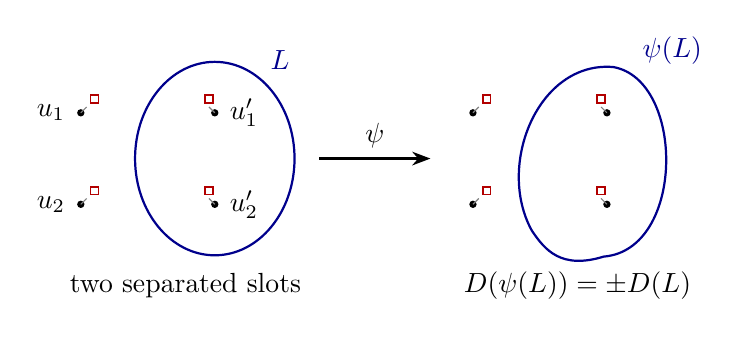
\begin{tikzpicture}[scale=.83,>=Stealth]
 \begin{scope}
  \draw[thick,blue!55!black] (0.8,0) ellipse (1.22 and 1.48);
  \node[blue!55!black] at (1.8,1.5) {$L$};
  \foreach \y/\j in {.7/1,-.7/2}{
   \fill (-1.25,\y) circle (1.6pt);
   \fill (.8,\y) circle (1.6pt);
   \node[anchor=east] at (-1.34,\y) {$u_{\j}$};
   \node[anchor=west] at (.88,\y) {$u'_{\j}$};
   \draw[gray,densely dashed] (-1.25,\y)--(-1.1,\y+.15);
   \draw[gray,densely dashed] (.8,\y)--(.65,\y+.15);
   \draw[red!70!black,fill=white,semithick] (-1.1,\y+.15) rectangle ++(.12,.12);
   \draw[red!70!black,fill=white,semithick] (.65,\y+.15) rectangle ++(.12,.12);
  }
  \node at (.35,-1.95) {two separated slots};
 \end{scope}
 \draw[->,thick] (2.4,0)--(4.1,0)
        node[midway,above] {$\psi$};
 \begin{scope}[xshift=6cm]
  \draw[thick,blue!55!black]
      (-.35,-1.1) .. controls (-.9,-.1) and (-.25,1.5) .. (.9,1.4)
      .. controls (2,1.2) and (2,-1.4) .. (.75,-1.5)
      .. controls (.1,-1.7) and (-.15,-1.4) .. (-.35,-1.1);
  \node[blue!55!black] at (1.8,1.65) {$\psi(L)$};
  \foreach \y/\j in {.7/1,-.7/2}{
   \fill (-1.25,\y) circle (1.6pt);
   \fill (.8,\y) circle (1.6pt);
   \draw[gray,densely dashed] (-1.25,\y)--(-1.1,\y+.15);
   \draw[gray,densely dashed] (.8,\y)--(.65,\y+.15);
   \draw[red!70!black,fill=white,semithick] (-1.1,\y+.15) rectangle ++(.12,.12);
   \draw[red!70!black,fill=white,semithick] (.65,\y+.15) rectangle ++(.12,.12);
  }
  \node at (.35,-1.95) {$D(\psi(L))=\pm D(L)$};
 \end{scope}
\end{tikzpicture}
\caption{Nearby nails (squares) detect the separations of endpoint
pairs (dots).  The homotopy bijection preserves oriented winding
differences.  A single sign change of a loop's whole separation
vector cancels when that loop occurs an even number of times.}
\label{fig:rr-nails}
\end{figure}

\subsection{Transfer of the correlation polynomial}

Fix $\alpha\in(0,\pi)$ and compact $K\subset\mathcal D_k$.
Choose $0<r<d_K/1000$.  Apply Lemma~\ref{lem:rr-nails} and, for
each endpoint, select an indexed nail close to it.  For all small
enough meshes both corresponding nails lie within $r/2$ of that
endpoint.  Nails selected for endpoints in distinct slots are
distinct.  In both samples discard the event that a loop of
diameter at least $d_K/4$ comes within $r$ of an endpoint.
Lemma~\ref{lem:rr-estimates} bounds the probability of these
exceptions by $C_K(r/d_K)^\gamma+o(1)$, uniformly for the
individual tuples in $K$.

On the remaining event, a relevant loop $L$ surrounds the nails
near one endpoint of each of two distinct slots, and excludes a
nail near the other endpoint of a separated slot.  It is therefore
non-trivial in the exact sense of Lemma~\ref{lem:rr-nails}, so
$\psi(L)$ is defined.  For those two slots the winding differences
at the corresponding nails are nonzero by
\eqref{eq:rr-winding-difference}.  Thus $\psi(L)$ separates each
of the two nail pairs.  In particular, it encloses one nail from
each of two distinct slots, whose distance is at least
$d_K-O(r+\delta)$.  This proves that $\psi(L)$ itself has diameter
at least $d_K/4$.  Its endpoint-avoidance event is consequently
applicable; smallness of the partner has not been assumed away.

Endpoint indicators and nearby-nail indicators agree for both
loops, as illustrated in Figure~\ref{fig:rr-nails}.
Equation~\eqref{eq:rr-winding-difference} now gives,
for \emph{every} slot,
\begin{equation}
 D_i(\psi(L))=\frac{s_L}{s_{\psi(L)}}D_i(L).
 \label{eq:rr-signature}
\end{equation}
The inverse bijection gives the same statement starting with a
relevant loop in the second sample.  Hence it is a bijection
between all relevant loops, preserving their entire separation
vectors up to one sign per loop.  For a block $B$ in an even
partition,
\[
 \prod_{i\in B}D_i(\psi(L))
    =\left(\frac{s_L}{s_{\psi(L)}}\right)^{|B|}
                       \prod_{i\in B}D_i(L)
    =\prod_{i\in B}D_i(L).
\]
Transporting the injective labels in
\eqref{eq:rr-even-polynomial} therefore makes the two polynomials
\emph{exactly equal} on the good event.  This uses the actual
bijection, so distinct loops are never identified with one another.
Cauchy--Schwarz and \eqref{eq:rr-UI} bound the expectation error by
$C_K(r/d_K)^{\gamma/2}+o(1)$.

It remains to pass from the auxiliary mixed samples to the intended
homogeneous ones.  Fix $R>10M$ and couple their restrictions
identically in $B(0,R)$ using the local-law assertion of
Lemma~\ref{lem:rr-nails}; for small enough mesh this disk lies in
both homogeneous windows.  Off the escaping-loop event in either
sample, all relevant complete loops are identical.  Equations
\eqref{eq:rr-escape} and \eqref{eq:rr-UI} bound the expectation
error by $C_K(M/R)^{\gamma/2}$.  Let the mesh tend to zero,
then $r\downarrow0$ and $R\uparrow\infty$.  Writing
$\Phi^{\alpha}_{k,\delta}$ for the fair-signed correlation on
$\delta\mathbb L(\alpha)$, we obtain
\begin{equation}
 \lim_{\delta\downarrow0}\sup_{\boldsymbol u\in K}
 \left|\Phi^{\pi/2}_{k,\delta}(\boldsymbol u)
                   -\Phi^{\alpha}_{k,\delta}(\boldsymbol u)\right|=0.
 \label{eq:rr-isoradial-transfer}
\end{equation}
No diameter threshold needs to be a continuity point: all small
loops were removed by the even-moment identity itself.

\begin{proof}[Proof of Theorem~\ref{thm:rr-rotation}]
The rectangular model on $\mathbb L(\alpha)$ is invariant under
reflection $S_{\alpha/2}$ about $e^{i\alpha/2}\R$
\cite[Remark~1.8]{DCKKMO2026Rotation}.  Its fair-sign height
correlations inherit that symmetry.  If the chosen endpoint
rounding is not reflection equivariant, the reflected
representatives differ by $O(\delta)$, which is harmless by
\eqref{eq:rr-continuity}.  Apply
\eqref{eq:rr-isoradial-transfer} at the original and reflected
tuples.  The square model is consequently asymptotically invariant
under $S_{\alpha/2}$, uniformly on every compact subset of
$\mathcal D_k$.  Composing with its exact horizontal-reflection
symmetry yields invariance under rotation through $\alpha$.
Square symmetries cover the endpoints and the other half of the
circle.  This proves the assertion for each fixed rotation.

The estimate \eqref{eq:rr-continuity} upgrades this to uniformity
in the rotation angle.  Indeed, the orthogonal images of $K$ form
a compact subset of $\mathcal D_k$, and a finite angular net
approximates every rotation with endpoint displacement at most
$C_K$ times its angular mesh.  First use convergence at the
finitely many net angles, and then let the angular mesh decrease.
Reflections follow by composition with an exact square symmetry.
This argument requires no estimate uniform in a degenerating
isoradial angle.

Finally, any translation differs from a period translation of the
mesh-$\delta$ square lattice by a vector of length $O(\delta)$.
Exact period invariance and the location-uniform estimate
\eqref{eq:rr-continuity} handle this residual displacement,
uniformly over \emph{all} translation vectors.  Every plane
isometry is a translation followed by an orthogonal map.
The fixed rotation and dilation identifying
$\mathbb L(\pi/2)$ with $\Z^2$ merely change the mesh convention
and compact set.  These observations prove
\eqref{eq:rr-target} for the original square lattice.
\end{proof}


\subsection{The endpoint field and all test classes}

\begin{proposition}[Completion at the endpoint]
\label{prop:endpoint-completion}
The conclusions of Theorem~\ref{thm:main} hold at $c=2$, with squared
multiplier $2/\pi$.
\end{proposition}

\begin{proof}
Lemma~\ref{lem:rr-bkw} identifies the fair unit-jump height with the
prescribed balanced plane law. Theorem~\ref{thm:rr-rotation} supplies
\cite[Theorem~4.1]{DKLM2026} at $c=2$; odd correlations vanish by
arrow reversal. We can therefore follow the isotropic argument of
that paper with its symmetry premise now proved here.

Specifically, \cite[Theorems~6.1, 7.1 and~8.1]{DKLM2026} give this
alternative: either the field converges to a fixed GFF multiple in all
three senses of its Definitions~2.5--2.7, or two mesh sequences give
GFF limits with distinct nonnegative multipliers. These senses include
separated correlations, finite-energy tests and the outward completion.
The free-energy identification in its Theorems~4.3--4.4 gives every
possible squared multiplier as
\[
 \sigma^2=-\frac1{f''(0)}
          =\frac2{\arccos(-1)}=\frac2\pi.
\]
Thus the alternative with two distinct multipliers is excluded, and
convergence holds along the full mesh limit.

Proposition~\ref{prop:endpoint-topologies} now applies to the
finite-energy convergence. Using the lattice-cutoff estimate of
\cite[Theorem~4.5]{DKLM2026}, it proves convergence and tightness
in the ordinary restriction and intrinsic negative topologies on
every bounded open set, with the common chosen pin. Its proof
retains endpoints rounded to the same face and arbitrarily small
positive-area cells at the boundary.

Finally, the fixed similarity identifying the FK medial lattice
with $\Z^2$ changes the logarithmic Green kernel only by an
additive constant. Neutrality cancels that constant, so the
coefficient and test conclusions agree with Theorem~\ref{thm:main}.
\end{proof}

\bibliographystyle{plain}
\bibliography{references}
\end{document}
